% ==============================================================================
% EDC Book Chapter: The Weak-Sector Brane Interface
% A Mechanistic Pipeline from Bulk Relaxation to 3D Weak Outputs
% ==============================================================================

\documentclass[11pt,a4paper]{article}

% ─────────────────────────────────────────────────────────────────────────────
% Required packages
% ─────────────────────────────────────────────────────────────────────────────
\usepackage{amsmath,amssymb,amsfonts,amsthm}
\usepackage{enumitem}
\usepackage{booktabs}
\usepackage{longtable}
\usepackage{array}
\usepackage{multirow}
\usepackage{graphicx}
\usepackage{xcolor}
\usepackage{tikz}
\usetikzlibrary{positioning,arrows.meta,shapes.geometric,calc,decorations.pathmorphing,fit,backgrounds}
\usepackage{tcolorbox}
\tcbuselibrary{skins,breakable}
\usepackage{hyperref}
\usepackage{geometry}
\geometry{margin=1in}  % Match EDC Book v17.49

% ─────────────────────────────────────────────────────────────────────────────
% Epistemic tags
% ─────────────────────────────────────────────────────────────────────────────
\newcommand{\tagBL}{\textsuperscript{\textcolor{blue!70!black}{[BL]}}}
\newcommand{\tagDef}{\textsuperscript{\textcolor{green!50!black}{[Def]}}}
\newcommand{\tagP}{\textsuperscript{\textcolor{orange!80!black}{[P]}}}
\newcommand{\tagDc}{\textsuperscript{\textcolor{purple!70!black}{[Dc]}}}
\newcommand{\tagOpen}{\textsuperscript{\textcolor{red!70!black}{[OPEN]}}}

% ─────────────────────────────────────────────────────────────────────────────
% Box styles
% ─────────────────────────────────────────────────────────────────────────────
\tcbset{
  readerContract/.style={
    colback=blue!5, colframe=blue!50!black,
    fonttitle=\bfseries, title={Reader Contract}
  },
  guardrail/.style={
    colback=yellow!5, colframe=orange!60!black,
    fonttitle=\bfseries
  },
  falsifiability/.style={
    colback=red!5, colframe=red!40!black,
    fonttitle=\bfseries, title={Falsifiability Hooks}
  },
  mechanism/.style={
    colback=teal!5, colframe=teal!50!black,
    fonttitle=\bfseries
  }
}

% ─────────────────────────────────────────────────────────────────────────────
% Formal box environments for proofs/propositions
% ─────────────────────────────────────────────────────────────────────────────
\newtcolorbox{edcPostulateBox}[2]{
  colback=orange!5, colframe=orange!60!black,
  fonttitle=\bfseries, title={#1 \hfill {\small #2}},
  breakable
}
\newtcolorbox{edcDefinitionBox}[2]{
  colback=green!5, colframe=green!50!black,
  fonttitle=\bfseries, title={Definition: #1 \hfill {\small #2}},
  breakable
}
\newtcolorbox{edcPropositionBox}[2]{
  colback=purple!5, colframe=purple!50!black,
  fonttitle=\bfseries, title={Proposition: #1 \hfill {\small #2}},
  breakable
}
\newtcolorbox{edcLedgerBox}[2]{
  colback=blue!5, colframe=blue!50!black,
  fonttitle=\bfseries, title={Ledger: #1 \hfill {\small #2}},
  breakable
}
\newtcolorbox{edcConsequenceBox}[2]{
  colback=teal!5, colframe=teal!50!black,
  fonttitle=\bfseries, title={#1 \hfill {\small #2}},
  breakable
}
\newtcolorbox{edcWarningBox}[2]{
  colback=yellow!10, colframe=orange!70!black,
  fonttitle=\bfseries, title={Guardrail: #1},
  breakable
}

% ─────────────────────────────────────────────────────────────────────────────
% Document metadata
% ─────────────────────────────────────────────────────────────────────────────
\hypersetup{
  pdftitle={The Weak-Sector Brane Interface},
  pdfauthor={Igor Grcman},
  pdfkeywords={EDC, weak sector, brane interface, thick-brane microphysics}
}

\title{%
  \textbf{Chapter: The Weak-Sector Brane Interface}\\[0.3em]
  \large A Mechanistic Pipeline from Bulk Relaxation to 3D Weak Outputs
}
\author{%
  Igor Gr\v{c}man\\
  \small Elastic Diffusive Cosmology
}
\date{January 2026}

% ─────────────────────────────────────────────────────────────────────────────
\begin{document}
% ─────────────────────────────────────────────────────────────────────────────

\maketitle

\tableofcontents
\newpage

% ==============================================================================
\section{Reader Contract: What This Chapter Is and Is Not}
\label{sec:reader_contract}
% ==============================================================================

% ==============================================================================
% Section 1.1: Epistemic Framework and How to Read Chapter 1 (short)
% ==============================================================================
% NOTE: This is the SHORT chapter-level version. The full Reader Contract
% and Epistemic Standard are in the book-level frontmatter.
% ==============================================================================

\section{Epistemic Framework and Chapter Guide}
\label{sec:reader_contract}

This chapter follows the EDC Epistemic Standard (Framework v2.0). Each claim
carries one evidence label: \tagBL{} baseline, \tagDer{} derived, \tagDc{} derived
conditional, \tagI{} identified, \tagCal{} calibrated, \tagP{} proposed, \tagM{} math.
Canonical definitions: Preface.

\paragraph{Reading map.}
\begin{itemize}[nosep]
  \item \textbf{Section~\ref{sec:unified_pipeline}} defines the canonical weak-sector
        pipeline used throughout this Part.
  \item \textbf{Sections~\ref{sec:case_neutron}--\ref{sec:case_neutrino}} apply that
        pipeline to concrete decay cases, specifying only case-dependent inputs.
  \item \textbf{Section~\ref{sec:gf_pathway}} explains the structural pathway toward
        an effective coupling ($G_F$).
  \item \textbf{Section~\ref{sec:epistemic_map}} collects all unresolved items
        (Consolidated Open Problems).
\end{itemize}

\paragraph{One-line rule.}
If a concept is defined elsewhere, we reference it rather than re-explain.
Pipeline = \S\ref{sec:unified_pipeline};
SM$\leftrightarrow$EDC bridge = \S\ref{sec:gf_pathway};
Open problems = \S\ref{sec:epistemic_map}.



% ==============================================================================
\section{How We Got Here: From 5D Relaxation to Brane-Interface Mechanics}
\label{sec:how_we_got_here}
% ==============================================================================

% ==============================================================================
% Section 1: How We Got Here
% ==============================================================================

This section answers the question that every careful reader should ask: ``How did we
arrive at this brane-interface picture, and why is it not merely an arbitrary
construction?''

\subsection{What We Are Trying to Explain (and What We Are Not)}

In the Standard Model, ``weak interactions'' are encoded as fundamental vertices and
gauge boson exchange. The $W^\pm$ and $Z^0$ bosons mediate weak processes, and the
interaction strength is set by the Fermi constant $G_F$ \tagBL{}.

In EDC, we pursue a different explanatory target: we aim to describe the observed
weak-sector phenomena as the \emph{observer-facing residue} of a bulk-to-brane transfer
process in a thick-brane geometry \tagP{}/\tagDc{}.

This chapter therefore does \emph{not} attempt a full Standard-Model derivation.
Instead, we build a mechanistic pipeline that is:
\begin{enumerate}[nosep]
  \item dimensionally consistent,
  \item explicit about what is baseline data versus hypothesis,
  \item structured so that future numerical closure remains well-defined rather than
        hidden inside language.
\end{enumerate}

\subsection{Why ``Weak'' Is Not a Fundamental Vertex in EDC}

The Standard Model treats weak interactions as arising from $SU(2)_L$ gauge symmetry.
The ``weakness'' comes from the large $W$ mass ($\sim 80$ GeV) appearing in propagator
denominators at low energies.

EDC offers a different interpretation \tagP{}:
\begin{quote}
\emph{Weak interactions are not fundamental vertices but the low-energy residue of
bulk$\to$brane energy transfer, geometrically suppressed by mediator gaps and
wavefunction overlaps.}
\end{quote}

This is not a claim that the Standard Model is wrong. Rather, it is a claim that
the Standard Model's effective description may have a deeper geometric origin in
a thick-brane microphysics.

\subsection{Why a Thick Brane Is Essential (Not Optional)}

A common simplification in extra-dimensional models is to treat the brane as a
delta-function localization. EDC requires a \emph{thick} brane for three essential
reasons \tagDc{}:

\paragraph{1. A reservoir for energy storage and redistribution.}
Bulk relaxation can pump energy into the brane layer, where it can be temporarily
stored and then redistributed among brane-layer modes before any 3D ``particle''
output is projected. A zero-thickness brane has no such storage capacity.

\paragraph{2. Mode overlap and localization.}
Effective couplings become overlap integrals of mode profiles across the brane
thickness. This provides a natural, geometric route to ``small effective couplings''
without inserting small numbers by hand \tagOpen{}.

\paragraph{3. A boundary/projection stage.}
The observer does not read off raw 5D fields. Instead, outputs are produced after
a ``frozen'' projection step (the observer-facing boundary condition), which can
enforce selection rules (including chirality selection) as a boundary phenomenon
\tagP{}/\tagOpen{}.

\subsection{Connecting to Observable Weak Phenomena}

The phenomena we must explain include \tagBL{}:

\begin{itemize}
  \item \textbf{Neutron $\beta$-decay}: $n \to p + e^- + \bar\nu_e$ with
        $\tau_n \approx 879$ s
  \item \textbf{Muon decay}: $\mu^- \to e^- + \bar\nu_e + \nu_\mu$ with
        $\tau_\mu \approx 2.2 \times 10^{-6}$ s
  \item \textbf{Tau decay}: Multiple channels (leptonic and hadronic) with
        $\tau_\tau \approx 2.9 \times 10^{-13}$ s
  \item \textbf{Pion decay}: $\pi^+ \to \mu^+ + \nu_\mu$ (dominant) with strong
        helicity suppression of the electron channel
  \item \textbf{Electron stability}: The lightest charged lepton does not decay
  \item \textbf{Neutrino properties}: Nearly massless, only left-handed coupling
        to weak currents
\end{itemize}

Each of these phenomena will receive a mechanistic interpretation in the case
studies (\S\ref{sec:case_studies}). The key insight is that they all share a
common interface logic: energy arrives from a bulk-facing process, is processed
in a thick-brane layer, and is then projected through boundary conditions into
an allowed set of 3D observable outputs.

\subsection{From Apparent Vertex to Coarse-Grained Residue}

In this mechanistic picture, a low-energy effective interaction term in 3D
should be read as a \emph{coarse-grained residue} of 5D transfer, not as a
fundamental interaction at a point \tagDc{}.

This is the logic behind the structural derivation of an effective four-fermion
coupling (see \S\ref{sec:GF_structural}): one couples a brane-facing current $J(x)$
to a mediator field supported in the thick brane; integrating out the mediator
produces a local contact term $J \cdot J$ with suppression controlled by mediator
gap and geometric overlap---not a tunable ``weak strength.''

The program is therefore:
\begin{enumerate}
  \item Identify the bulk-facing trigger for each weak process
  \item Describe the brane-charging (absorption) stage
  \item Characterize the mode redistribution (dissipation) stage
  \item Apply the frozen projection operator (release) to obtain 3D outputs
  \item Check that the energy ledger closes and selection rules are respected
\end{enumerate}

This is what we mean by ``mechanistic'': not a black box labeled ``weak vertex,''
but an explicit causal chain from 5D dynamics to 3D observation.


% ==============================================================================
\section{Geometry and Interface: The Continuum of 4D Submanifolds in 5D}
\label{sec:geometry_interface}
% ==============================================================================

% ==============================================================================
% Section 1.3: Geometry and Interface
% ==============================================================================

\section{Geometry of the Brane Interface}
\label{sec:geometry_interface}

This section addresses a fundamental question: in a 5D bulk, how does our particular
4D universe get selected, and what makes weak-sector mechanics possible?

\subsection{The Continuum of 4D Submanifolds in 5D}

Geometrically, a 5D manifold contains a continuum of possible 4D submanifolds.
If we parameterize the fifth dimension by a coordinate $\xi$, then surfaces of
constant $\xi$ are 4D hypersurfaces. But the geometry is richer: 4D submanifolds
can have arbitrary orientations, curvatures, and embeddings.

The question is: \emph{why does physics select a particular 4D hypersurface as
``our universe''?}

In delta-function brane models, this is typically assumed rather than derived.
In EDC's thick-brane picture, the selection arises from \emph{dynamics}: the
brane is not imposed but emerges as a stable interface configuration \tagP{}.

\subsection{Mechanistic Selection: Boundary Conditions and Couplings}

Not every 4D submanifold can support the physics we observe. The EDC dynamics
selects a specific interface through \tagDc{}:

\paragraph{1. Boundary conditions.}
The brane has two faces: a bulk-facing (Plenum-facing) side at $y = -\delta/2$
and an observer-facing side at $y = +\delta/2$. Each face carries boundary
conditions that determine what modes can propagate and what couplings are allowed.

\paragraph{2. Coupling structure.}
The effective 4D couplings arise from overlap integrals of 5D mode profiles
across the brane thickness. This structure is not free: it is constrained by
the 5D dynamics and boundary conditions.

\paragraph{3. Stability requirements.}
The interface must be stable against small perturbations. An unstable interface
would not persist long enough to support the observed physics.

\subsection{The Viability Filter: What Makes a Universe Observable?}

We propose that the interface we call ``our universe'' satisfies a set of
\emph{viability conditions} \tagP{}/\tagDc{}:

\begin{tcolorbox}[guardrail, title={Viability Filter Conditions}]
\begin{enumerate}
  \item \textbf{Proton-Anchor Stability} \tagP{}:
        The proton configuration (modeled as a Y-junction in the brane layer)
        must be a stable minimum-energy topology. Without a stable anchor,
        there is no stable matter and no observers.

  \item \textbf{Ledger Closure}:
        Energy and quantum numbers must be conserved across the bulk$\to$brane$\to$3D
        pipeline. Without ledger closure, the mechanism is not self-consistent.

  \item \textbf{Suppressed Leakage} \tagP{}:
        Bulk modes must not leak freely into the 3D sector. If everything leaked,
        there would be no selection rules and no structured particle spectrum.
\end{enumerate}
\end{tcolorbox}

These conditions are not arbitrary: they are necessary for the existence of
stable matter and observable weak processes.

\subsection{Proton-Anchor Stability Principle}

\begin{tcolorbox}[mechanism, title={Proton-Anchor Stability}]
\textbf{Postulate} \tagP{}:
Our universe is stable because the proton Y-junction configuration represents a
local minimum of the 5D energy functional. The proton is not just ``the lightest
baryon''; it is the \emph{topological anchor} that stabilizes the brane-observer
interface.

\textbf{Consequence} \tagDc{}:
If the proton were unstable, baryonic matter would decay, and the conditions for
complex chemistry and observers would not persist.
\end{tcolorbox}

\paragraph{Falsifiability.}
This principle is falsifiable: if proton decay were observed with a lifetime
shorter than $\sim 10^{34}$ years \tagBL{}, the claim that the proton is a
stable anchor would require revision.

\paragraph{What this explains.}
The proton-anchor principle explains why EDC treats the neutron-to-proton
transition as a \emph{relaxation toward a stable minimum} rather than an
arbitrary decay. The proton is the endpoint because it is the stable configuration.

\subsection{Generative Closure Principle}
\label{sec:generative_closure_principle}

\begin{tcolorbox}[mechanism, title={Generative Closure}]
\textbf{Postulate} \tagP{}:
The electron sector (electron as ground-mode brane defect, neutrino as edge mode)
together with the proton anchor constitutes a \emph{closed generative substrate}.
All weak-sector outputs must be expressible in terms of these fundamental components.

\textbf{Consequence} \tagDc{}:
Weak decays do not produce arbitrary particles; they produce combinations of
$\{p, e^\pm, \nu, \bar\nu\}$ because these are the stable outputs allowed by
the interface mechanism.
\end{tcolorbox}

This principle constrains what can appear as a weak-sector output: not because
of an inserted selection rule, but because only certain modes survive the
projection through the observer-facing boundary.

\subsection{Where This Leads}

The geometry-interface picture establishes the \emph{arena} for weak-sector
dynamics. Section~\ref{sec:unified_pipeline} formalizes the \emph{mechanism}:
the unified pipeline (Absorption $\to$ Dissipation $\to$ Release) with explicit
energy flow, projection operators, and ledger closure requirements.


% ==============================================================================
\section{Unified Weak-Sector Pipeline: Absorption, Dissipation, Release}
\label{sec:unified_pipeline}
% ==============================================================================

% ==============================================================================
% Section 3: Unified Pipeline
% ==============================================================================

This section formalizes the Absorption $\to$ Dissipation $\to$ Release pipeline
that governs all weak-sector processes in EDC.

\subsection{Pipeline Overview: What Happens Physically}

We propose that weak-sector decays in EDC share a common mechanistic skeleton
\tagP{}/\tagDc{}:

\begin{center}
\fbox{\textbf{Absorption}} $\longrightarrow$
\fbox{\textbf{Dissipation}} $\longrightarrow$
\fbox{\textbf{Release}}
\end{center}

\noindent
The central claim is not that all decays have identical microphysics, but that
the \emph{interface logic} is shared: energy arrives from a bulk-facing process,
is processed in a thick-brane layer, and is then projected through boundary
conditions into an allowed set of 3D observable outputs.

\paragraph{Absorption (brane charging).}
Bulk-facing dynamics (e.g., junction relaxation, mode de-excitation) pump energy
into the brane layer. The brane acts as a reservoir that accumulates energy before
any 3D output is produced.

\paragraph{Dissipation (mode redistribution).}
The accumulated energy does not remain in its initial form. It redistributes among
the available brane-layer modes $\{\phi_k\}$. This stage is crucial: without it,
one cannot explain why the observed outputs appear as a restricted set rather than
an arbitrary energy dump.

\paragraph{Release (observer projection).}
The observer-facing boundary condition projects the brane-layer modes into 3D
outputs. This projection is \emph{not} the identity: it filters modes according
to kinematic, topological, and chirality constraints.

\subsection{Energy-Flow Bookkeeping}

We describe the brane layer as an intermediate reservoir carrying an energy
content $E_{\text{brane}}(t)$ \tagDef{}. Energy conservation at the level of
the reservoir is captured by:
\begin{equation}
\frac{dE_{\text{brane}}}{dt} \;=\; \Pi_{\text{pump}}(t) \;-\; \Pi_{\text{release}}(t)
\;-\; \Pi_{\text{other}}(t),
\label{eq:brane_energy_balance}
\end{equation}
where:
\begin{itemize}[nosep]
  \item $\Pi_{\text{pump}}$ is the bulk$\to$brane pumping power \tagDef{},
  \item $\Pi_{\text{release}}$ is the brane$\to$3D release power \tagDef{},
  \item $\Pi_{\text{other}}$ captures additional channels (recoil, soft emission,
        bulk residual) \tagDef{}/\tagOpen{}.
\end{itemize}

\paragraph{Dimensional check.}
All $\Pi$ quantities have dimensions of \textbf{energy/time} (power). The energy
balance equation is dimensionally consistent: $[E]/[t] = [E/t]$.

\subsection{Pumping Power: A Practical Model}

In the effective 1D brane-coordinate description, the pumping power is represented
as \tagDef{}:
\begin{equation}
\Pi_{\text{pump}}(t) \;\equiv\; -\dot{q}(t) \cdot \partial_q V(q(t)),
\label{eq:pump_power_def}
\end{equation}
where $q(t)$ is an effective collective coordinate (e.g., junction position) and
$V(q)$ is an effective potential. This has units of energy/time and corresponds
to the instantaneous power associated with motion along $V(q)$.

\paragraph{Physical interpretation.}
As a bulk-facing configuration relaxes toward a minimum of $V(q)$, it converts
potential energy into kinetic energy, which then pumps into the brane layer.
The pumping ceases when the system reaches the minimum ($\dot{q} \to 0$) or when
$\partial_q V \to 0$.

\subsection{Regime Parameter and Trigger Condition}

A useful dimensionless discriminator between ``still being pumped'' and
``effectively releasing'' is \tagDef{}:
\begin{equation}
\Xi(t) \;\equiv\; \frac{\Pi_{\text{pump}}(t)}{\Pi_{\text{release}}(t)}.
\label{eq:Xi_def}
\end{equation}

\paragraph{Regime interpretation.}
\begin{itemize}
  \item $\Xi \gg 1$: Pumping-dominated regime. Energy accumulates in the brane.
  \item $\Xi \sim 1$: Transition regime. Pumping and release are comparable.
  \item $\Xi \ll 1$: Release-dominated regime. The brane empties into 3D outputs.
\end{itemize}

The \textbf{freeze/release trigger} is the transition to the release-dominated
regime \tagDc{}:
\begin{equation}
t = t_*: \qquad \Xi(t_*) \ll 1.
\label{eq:trigger_condition}
\end{equation}

\paragraph{Important nuance.}
We do not claim that $\dot{q}(t_*) = 0$ exactly. Rather, the interface becomes
\emph{effectively frozen} at observational resolution: the continuous pump term
is negligible, and the release can be treated as the dominant process. This is
a \emph{regime statement}, not an exact dynamical endpoint.

\subsection{The Frozen Projection Operator}

The key conceptual move is that the observer does not ``see'' raw 5D fields.
Instead, 3D outputs are those components that survive the observer-facing
projection. We write \tagDef{}:
\begin{equation}
\mathcal{P}_{\text{frozen}} \;=\;
\mathcal{P}_{\text{energy}} \circ \mathcal{P}_{\text{mode}} \circ \mathcal{P}_{\text{chir}},
\label{eq:Pfrozen_def}
\end{equation}
where:

\paragraph{$\mathcal{P}_{\text{energy}}$: Kinematic gate.}
Enforces kinematic admissibility: only channels with positive Q-value and
available phase space are allowed \tagDef{}/\tagBL{}. This is purely kinematic
and does not require EDC-specific assumptions.

\paragraph{$\mathcal{P}_{\text{mode}}$: Mode-to-output mapping.}
Maps brane-layer excitations to allowed output species channels. Which internal
modes can produce which particles is determined by the mode structure of the
thick brane \tagP{}/\tagOpen{}.

\paragraph{$\mathcal{P}_{\text{chir}}$: Chirality filter.}
Encodes chirality/helicity selection as a boundary condition effect. The V$-$A
structure of weak interactions emerges from the geometry of the observer-facing
boundary \tagP{}/\tagOpen{}.

\subsection{Output Definition}

The 3D output set is defined at the level of the pipeline as \tagDef{}:
\begin{equation}
\{\text{outputs}\}_{3D} \;\equiv\;
\mathcal{P}_{\text{frozen}}\big(\{\phi_k\}_{\text{brane modes}}\big).
\label{eq:outputs_def}
\end{equation}

\paragraph{Interpretation.}
This formulation makes explicit where ``weak selection rules'' live in EDC:
they are not inserted as vertices but emerge as an interface phenomenon governed
by reservoir dynamics, mode structure, and observer-facing projection.

\subsection{Ledger Closure Requirement}

For any process, the energy ledger must close \tagDef{}:
\begin{equation}
\Delta E_{\text{available}} \;=\;
\sum_{\text{outputs}} K_i \;+\; E_{\text{other}},
\label{eq:ledger_closure}
\end{equation}
where $K_i$ are the kinetic energies of 3D outputs and $E_{\text{other}}$
captures subleading channels (recoil, soft modes, bulk residual).

This is not a derived result but a \emph{consistency requirement}: any mechanism
that fails to close the ledger is incomplete or incorrect.

\subsection{Pipeline Summary Diagram}

The unified pipeline can be represented schematically as:

\begin{center}
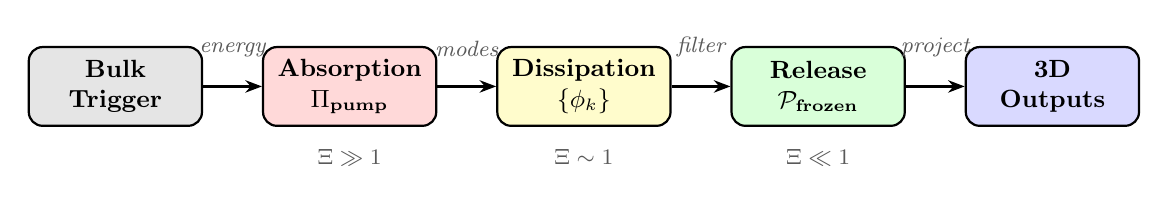
\begin{tikzpicture}[
  scale=0.85,
  box/.style={rectangle, rounded corners=5pt, minimum width=2.2cm, minimum height=1cm,
              draw=black, thick, font=\small\bfseries, align=center},
  arrow/.style={-{Stealth[length=6pt]}, thick},
  label/.style={font=\footnotesize\itshape, text=gray!70!black}
]
% Boxes
\node[box, fill=gray!20] (bulk) at (0,0) {Bulk\\Trigger};
\node[box, fill=red!15] (abs) at (3.5,0) {Absorption\\$\Pi_{\text{pump}}$};
\node[box, fill=yellow!20] (dis) at (7,0) {Dissipation\\$\{\phi_k\}$};
\node[box, fill=green!15] (rel) at (10.5,0) {Release\\$\mathcal{P}_{\text{frozen}}$};
\node[box, fill=blue!15] (out) at (14,0) {3D\\Outputs};

% Arrows
\draw[arrow] (bulk) -- (abs);
\draw[arrow] (abs) -- (dis);
\draw[arrow] (dis) -- (rel);
\draw[arrow] (rel) -- (out);

% Labels
\node[label, above] at (1.75,0.3) {energy};
\node[label, above] at (5.25,0.3) {modes};
\node[label, above] at (8.75,0.3) {filter};
\node[label, above] at (12.25,0.3) {project};

% Regime annotation
\node[label, below] at (3.5,-0.8) {$\Xi \gg 1$};
\node[label, below] at (7,-0.8) {$\Xi \sim 1$};
\node[label, below] at (10.5,-0.8) {$\Xi \ll 1$};
\end{tikzpicture}
\end{center}

This diagram applies to all weak processes considered in this chapter; the case
studies will fill in the specific triggers, modes, and outputs for each particle.


% ==============================================================================
\section{Particle Ontology in EDC}
\label{sec:ontology}
% ==============================================================================

% ==============================================================================
% Section 4: Particle Ontology in EDC
% ==============================================================================

Before diving into case studies, the reader needs a map of ``what is what'' in
EDC's 5D picture. This section classifies the particles of the weak sector by
their ontological status in the thick-brane geometry.

\subsection{Five Ontological Categories}

EDC classifies weak-sector particles into five categories based on their
geometric relationship to the thick brane \tagP{}/\tagDc{}:

\begin{table}[ht]
\centering
\begin{tabular}{llll}
\toprule
\textbf{Category} & \textbf{Examples} & \textbf{5D Character} & \textbf{Dominant Suppression} \\
\midrule
Bulk-core junction & Neutron & Extends into bulk & $\mathcal{P}_{\text{energy}}$ \\
Brane-dominant (fundamental) & $\mu$, $\tau$ & Localized in brane & $\mathcal{P}_{\text{mode}}$ \\
Brane defect & Electron & Ground-mode excitation & None (stable) \\
Edge mode & Neutrino & Interface-localized & $\mathcal{P}_{\text{chir}}$ \\
Composite & Pion & Junction pair & $\mathcal{P}_{\text{chir}}$ \\
\bottomrule
\end{tabular}
\caption{Ontological classification of weak-sector particles in EDC.}
\label{tab:ontology}
\end{table}

\subsection{Bulk-Core Junction: The Neutron}

\begin{tcolorbox}[mechanism, title={Neutron Ontology}]
\textbf{Definition} \tagP{}: The neutron is a \emph{bulk-core junction} configuration.
It is not purely brane-localized: part of its structure extends into the bulk, which
is why its decay involves relaxation of a bulk-facing component.

\textbf{Decay mechanism}: Junction relaxation pumps energy into the brane layer,
which then releases into $\{p, e^-, \bar\nu_e\}$.

\textbf{Key feature}: The neutron's bulk-facing character makes it the natural
``anchor case'' for the weak program: it provides the clearest example of
bulk$\to$brane transfer.
\end{tcolorbox}

\subsection{Brane-Dominant Fundamental: Muon and Tau}

\begin{tcolorbox}[mechanism, title={Muon/Tau Ontology}]
\textbf{Definition} \tagP{}: The muon and tau are \emph{brane-dominant excitations}.
They are localized within the thick brane layer and represent excited modes of the
same fundamental sector that has the electron as its ground state.

\textbf{Decay mechanism}: Mode de-excitation within the brane releases energy into
lower-lying modes plus neutrinos.

\textbf{Key feature}: No hadrons on leading order---the mode mismatch
$\mathcal{P}_{\text{mode}}$ prevents hadronic output for the muon. For the tau,
higher energy opens hadronic channels.
\end{tcolorbox}

The muon and tau are distinguished by their mode index: the tau occupies a higher
excited state, which explains both its larger mass and its additional decay channels.

\subsection{Brane Defect: The Electron}

\begin{tcolorbox}[mechanism, title={Electron Ontology}]
\textbf{Definition} \tagP{}: The electron is the \emph{ground-mode brane defect}.
It is the lowest-energy charged excitation of the brane layer.

\textbf{Stability mechanism}: There is no lower-energy charged state into which
the electron could decay. The ledger cannot close without violating charge
conservation.

\textbf{Key feature}: The electron is stable not because of an inserted conservation
law, but because the thick-brane mode structure has no lower-lying charged mode.
\end{tcolorbox}

\subsection{Edge Mode: The Neutrino}

\begin{tcolorbox}[mechanism, title={Neutrino Ontology}]
\textbf{Definition} \tagP{}: The neutrino is an \emph{edge mode} localized at the
bulk-brane interface. It does not penetrate deeply into either the bulk or the
brane interior.

\textbf{Weak coupling mechanism}: The neutrino's interface localization means its
overlap with bulk and brane-interior modes is suppressed. This is the geometric
origin of ``weak interactions'' for neutrinos.

\textbf{Chirality}: The interface geometry naturally selects left-handed neutrinos
for coupling. This is encoded in $\mathcal{P}_{\text{chir}}$.
\end{tcolorbox}

\subsection{Composite: The Pion}

\begin{tcolorbox}[mechanism, title={Pion Ontology}]
\textbf{Definition} \tagP{}: The charged pion is a \emph{brane-dominant composite},
modeled as a junction-pair configuration (loosely, a bound $q\bar{q}$ state in
traditional language, but here arising from brane geometry).

\textbf{Decay mechanism}: The junction pair annihilates, releasing energy into
$\ell + \nu$. The chirality projection $\mathcal{P}_{\text{chir}}$ enforces
helicity suppression.

\textbf{Key feature}: Helicity suppression factor $(m_e/m_\mu)^2$ is a baseline
fact \tagBL{}; EDC interprets it as a consequence of boundary conditions
\tagP{}/\tagOpen{}.
\end{tcolorbox}

\subsection{Ontology Map}

The following diagram shows how the five categories relate to the thick-brane
geometry:

\begin{center}
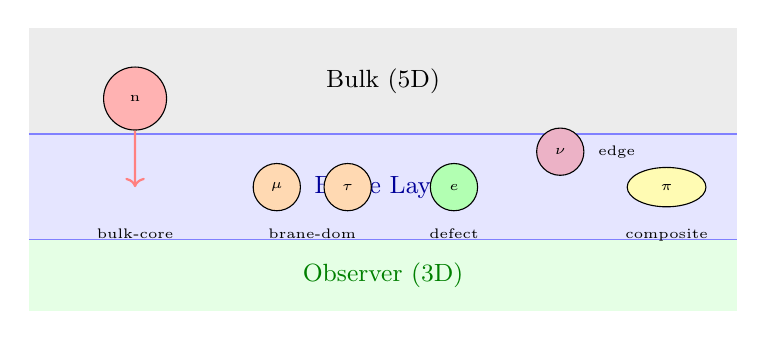
\begin{tikzpicture}[scale=0.9]
% Bulk region
\fill[gray!15] (-5,2) rectangle (5,3.5);
\node[font=\small] at (0,2.75) {Bulk (5D)};

% Brane layer
\fill[blue!10] (-5,0.5) rectangle (5,2);
\draw[thick, blue!50] (-5,0.5) -- (5,0.5);
\draw[thick, blue!50] (-5,2) -- (5,2);
\node[font=\small, blue!60!black] at (0,1.25) {Brane Layer};

% Observer region
\fill[green!10] (-5,-0.5) rectangle (5,0.5);
\node[font=\small, green!50!black] at (0,0) {Observer (3D)};

% Particles
\node[draw, circle, fill=red!30, minimum size=0.8cm, font=\tiny] (n) at (-3.5,2.5) {n};
\draw[->, thick, red!50] (n) -- (-3.5,1.25);
\node[font=\tiny, below] at (-3.5,0.8) {bulk-core};

\node[draw, circle, fill=orange!30, minimum size=0.6cm, font=\tiny] (mu) at (-1.5,1.25) {$\mu$};
\node[draw, circle, fill=orange!30, minimum size=0.6cm, font=\tiny] (tau) at (-0.5,1.25) {$\tau$};
\node[font=\tiny, below] at (-1,0.8) {brane-dom};

\node[draw, circle, fill=green!30, minimum size=0.6cm, font=\tiny] (e) at (1,1.25) {$e$};
\node[font=\tiny, below] at (1,0.8) {defect};

\node[draw, circle, fill=purple!30, minimum size=0.6cm, font=\tiny] (nu) at (2.5,1.75) {$\nu$};
\node[font=\tiny, right] at (2.9,1.75) {edge};

\node[draw, ellipse, fill=yellow!30, minimum width=1cm, minimum height=0.5cm, font=\tiny] (pi) at (4,1.25) {$\pi$};
\node[font=\tiny, below] at (4,0.8) {composite};
\end{tikzpicture}
\end{center}

Each category appears in its characteristic location: bulk-core junctions extend
into the bulk; brane-dominant modes and defects are localized within the brane;
edge modes sit at the interface; composites are structured configurations within
the brane.


% ==============================================================================
% Section: Proton as a Topological Anchor of the Brane--Observer Interface
% ==============================================================================

\subsection{Proton as a Topological Anchor of the Brane--Observer Interface}
\label{sec:proton_anchor}

\subsubsection{Statement (Postulate) and Consequence}

\begin{edcPostulateBox}{Proton-Anchor Stability Principle}{[P]/[Dc]}
\textbf{Postulate [P].} Our universe is stable because the proton Y-junction configuration represents
a \emph{local minimum} of an appropriate 5D energy functional under the thick-brane boundary conditions.
In EDC, the proton is not merely ``the lightest baryon''; it is a \emph{topological anchor} that stabilizes
the brane--observer interface.

\medskip
\textbf{Consequence [Dc].} If the proton were not (meta)stable as an anchored junction state,
baryonic matter would not persist, and the conditions required for complex chemistry and observers
would not be robust over macroscopic timescales.
\end{edcPostulateBox}

\subsubsection{Minimal Formal Setup: Energy Functional and Configuration Space}

We model baryonic candidates as defect configurations of the thick-brane microstructure.
Let $\mathcal{C}$ denote the space of admissible configurations (fields, embeddings, junction networks, and
their boundary data) consistent with the EDC interface conditions. We assume an effective 5D energy functional
\begin{equation}
\label{eq:5d_energy_functional}
\mathcal{E}[\Psi] \;=\; \mathcal{E}_{\mathrm{bulk}}[\Psi] \;+\; \mathcal{E}_{\mathrm{brane}}[\Psi] \;+\; \mathcal{E}_{\mathrm{BC}}[\Psi],
\end{equation}
where $\Psi\in\mathcal{C}$ encodes the relevant degrees of freedom (bulk/plenum variables, brane-layer modes,
and interface constraints). The precise microscopic form is left \textbf{OPEN} (see \S\ref{sec:proton_open_targets});
here we only require that $\mathcal{E}$ be well-defined on $\mathcal{C}$ and admits stationary points.

\subsubsection{Topological Classes and the Junction Number}

The key point is that not all deformations of a defect network are equivalent: there exist topological classes
(e.g.\ homotopy classes) that cannot be continuously deformed into one another without crossing a high-energy barrier
or violating boundary constraints. We therefore partition $\mathcal{C}$ into disjoint sectors,
\begin{equation}
\label{eq:topological_sectors}
\mathcal{C} \;=\; \bigsqcup_{\alpha\in\mathcal{I}} \mathcal{C}_\alpha,
\end{equation}
where the index $\alpha$ labels a conserved topological invariant (``junction charge'', ``winding'', or an equivalent
classification appropriate to the EDC microphysics).

\begin{edcDefinitionBox}{Y-junction sector}{[Def]}
We define the \emph{Y-junction sector} $\mathcal{C}_{Y}$ as the class of configurations whose defect network has one
trivalent junction with three legs (``arms'') satisfying the brane-interface boundary conditions on the observer-facing side.
\end{edcDefinitionBox}

\subsubsection{Local Minimality as a Stability Criterion}

Stability in this context means: within the same topological sector, small admissible perturbations cannot reduce the energy.
Formally, for a candidate configuration $\Psi_\star\in\mathcal{C}_{Y}$:

\begin{edcDefinitionBox}{Local minimum}{[Def]}
$\Psi_\star$ is a \emph{local minimum} of $\mathcal{E}$ on $\mathcal{C}_Y$ if there exists $\varepsilon>0$ such that
for all $\Psi\in\mathcal{C}_Y$ with $\|\Psi-\Psi_\star\|<\varepsilon$, one has
$\mathcal{E}[\Psi]\ge \mathcal{E}[\Psi_\star]$.
\end{edcDefinitionBox}

\subsubsection{Proposition and Proof Sketch}

\begin{edcPropositionBox}{Proton as a locally minimizing Y-junction}{[P]/[Dc]}
Assume (i) the Y-junction sector $\mathcal{C}_Y$ is topologically separated from the trivial sector $\mathcal{C}_0$ by an
energy barrier (no continuous unwinding under the BCs), and (ii) within $\mathcal{C}_Y$ the functional $\mathcal{E}$
admits a stationary configuration $\Psi_p$ whose second variation is positive for all admissible perturbations.
Then $\Psi_p$ is a local minimum of $\mathcal{E}$ in $\mathcal{C}_Y$ and represents a metastable anchored state
(the proton), providing a robust brane--observer stabilizer.
\end{edcPropositionBox}

\begin{proof}[Proof sketch (mechanistic/topological)]
\textbf{Step 1 (stationarity).} Solve $\delta\mathcal{E}[\Psi]=0$ within $\mathcal{C}_Y$ under the boundary conditions.
This yields a candidate junction configuration $\Psi_p$.

\textbf{Step 2 (topological protection).} Because $\mathcal{C}_Y$ and $\mathcal{C}_0$ are disjoint sectors,
any path from $\Psi_p$ to a trivial/no-junction state must cross configurations that violate the BCs or incur a large
energy cost. This prevents ``unwinding'' by small perturbations.

\textbf{Step 3 (local minimality).} Evaluate the second variation $\delta^2\mathcal{E}[\Psi_p;\eta]$ for admissible
perturbations $\eta$ that preserve the Y-sector constraints. If $\delta^2\mathcal{E}[\Psi_p;\eta] > 0$ for all such $\eta$,
then $\Psi_p$ is a strict local minimum within $\mathcal{C}_Y$.

\textbf{Step 4 (stability consequence).} A locally minimizing, topologically protected junction state persists against
small disturbances and acts as an anchor for the observer-facing interface; without such an anchor, baryonic composites
would not be robust. This is the mechanism-level sense in which proton stability underwrites chemistry and observers.
\end{proof}

\subsubsection{Forward Reference: The $\mathbb{Z}_6$ Program (Chapter 2)}

The proof sketch above outlines \emph{what} must be true for proton stability. In \textbf{Chapter~2}
(``The $\mathbb{Z}_6$ Program''), we provide the complete geometric derivation of \emph{why} this is true.
Specifically, Chapter~2 establishes:

\begin{itemize}[nosep]
  \item The proton Y-junction emerges as a $\mathbb{Z}_3$ fixed point of the hexagonal lattice symmetry
  \item The 120° Steiner angles are geometrically \emph{inevitable} from $\mathbb{Z}_6$-invariant boundary conditions
  \item The positive Hessian (local minimum) follows from the crystallographic structure
  \item The neutron is identified as a \emph{dislocation} in this lattice, explaining its instability
  \item Color confinement emerges from $\mathbb{Z}_3$ charge conservation
\end{itemize}

\noindent
The derivation chain in Chapter~2 transforms the [P] status of this section into [Dc] (derived consequence).
This chapter presents the \emph{physics and mechanism}; Chapter~2 provides the \emph{mathematical proof}.

\subsubsection{Connection to the Continuum of 4D Interfaces}

Among the continuum of possible 4D interfaces embedded in the 5D bulk, only those admitting a stable
topological anchor plus ledger closure yield observer-robust worlds. The proton Y-junction is one
concrete stabilizer that makes \emph{our} interface long-lived.

This connects to the broader EDC picture:
\begin{itemize}[nosep]
  \item 5D contains a continuum of 4D submanifolds (different ``interface'' choices)
  \item A viability filter selects which interfaces can be stable
  \item The proton anchor is the baryonic component of this stability
  \item The electron/neutrino pair (see \S\ref{sec:generative_closure_principle}) provides the leptonic component
\end{itemize}

\subsubsection{What Must Be Explicitly Closed (OPEN Targets)}
\label{sec:proton_open_targets}

This section is \emph{mechanism-complete} but not yet \emph{numerically closed}. The following closures remain OPEN:

\begin{itemize}[nosep]
\item \textbf{OPEN-Pa1:} Specify the concrete microphysical degrees of freedom $\Psi$ used in $\mathcal{E}[\Psi]$.
\item \textbf{OPEN-Pa2:} Derive the explicit boundary conditions at the brane--observer interface that define $\mathcal{C}_Y$.
\item \textbf{OPEN-Pa3:} Construct the topological invariant $\alpha$ (junction charge/winding) that partitions $\mathcal{C}$.
\item \textbf{OPEN-Pa4:} Compute (analytically or numerically) $\delta^2\mathcal{E}$ around $\Psi_p$ to verify positivity.
\item \textbf{OPEN-Pa5:} Estimate the barrier height between $\mathcal{C}_Y$ and $\mathcal{C}_0$ (metastability timescale).
\end{itemize}

\subsubsection{Falsifiability Hooks}

\begin{tcolorbox}[falsifiability]
\begin{itemize}[nosep]
  \item If proton decay is observed at rates inconsistent with a topologically protected minimum, the
        anchor mechanism fails.
  \item If the Y-junction configuration cannot be realized as a stationary point of any reasonable
        5D energy functional, the structural claim is falsified.
  \item If the second variation $\delta^2\mathcal{E}$ has negative eigenvalues (unstable directions),
        the local-minimum claim fails.
  \item If baryonic matter can be destabilized by small perturbations without violating conservation
        laws, the topological protection is illusory.
\end{itemize}
\end{tcolorbox}



% ==============================================================================
% Section: Neutron as an Excited Junction on a Proton-Anchored Interface
% ==============================================================================

\subsection{Neutron as an Excited Junction on a Proton-Anchored Interface}
\label{sec:neutron_story}

\subsubsection{Why the Proton Anchor Matters for Neutron Physics (Mechanistic Continuity)}

The Proton-Anchor Stability Principle (\S\ref{sec:proton_anchor}) is not a philosophical add-on;
it is the \emph{mechanical prerequisite} for defining any long-lived observer-facing weak process.
If the brane--observer interface were not stabilized by a locally minimizing topological anchor,
then junction excitations would not admit a consistent separation between:
\begin{enumerate}[nosep]
  \item[(i)] a metastable ``ground'' configuration (proton-like anchor),
  \item[(ii)] a nearby excited configuration (neutron-like junction state), and
  \item[(iii)] an observer-facing release map that conserves the ledger.
\end{enumerate}

In EDC language: the proton provides the \emph{stable reference sector} in configuration space
against which neutron decay can be defined as a relaxation process, rather than an arbitrary fitted timer.

\subsubsection{Neutron Ontology: A Bulk-Core Excitation Above the Anchored Junction}

\begin{edcDefinitionBox}{Neutron state as a junction excitation}{[Dc]}
We treat the neutron as a bulk-core junction excitation: a configuration $\Psi_n$ in the same broad
topological family as the anchored Y-junction, but displaced in the bulk-facing degrees of freedom.
The proton corresponds to a locally minimizing configuration $\Psi_p$ (anchor),
while the neutron corresponds to a higher-energy configuration $\Psi_n$ that can relax toward $\Psi_p$.
\end{edcDefinitionBox}

Mechanistically, the decay is not ``a weak vertex'' acting in 3D; it is the \emph{completion of a 5D relaxation}:
a bulk-facing excitation relaxes toward the proton anchor while transferring (pumping) energy into the brane layer,
which then redistributes that energy and finally releases allowed 3D outputs.

\subsubsection{The Three-Phase Pipeline: Absorption $\to$ Dissipation $\to$ Release}

We reuse the unified pipeline established in the weak program:
\begin{equation}
\label{eq:unified_pipeline_neutron}
\text{Bulk relaxation} \;\Rightarrow\;
\underbrace{\Pi_{\mathrm{pump}}}_{\text{absorption into brane}}
\;\Rightarrow\;
\underbrace{\Gamma_{\mathrm{eff}}}_{\text{brane-layer dissipation}}
\;\Rightarrow\;
\underbrace{\mathcal{P}_{\mathrm{frozen}}}_{\text{release as 3D outputs}}.
\end{equation}

\paragraph{Absorption (charging) \tagDc{}.}
During relaxation, the bulk-facing configuration does work on brane-layer degrees of freedom.
In the 1D effective description (junction coordinate $q(t)$), the instantaneous pumping power is
\begin{equation}
\label{eq:pump_power_neutron}
\Pi_{\mathrm{pump}}(t) \;\equiv\; -\dot q(t)\,\partial_q V(q),
\qquad [\Pi_{\mathrm{pump}}]=\text{energy/time}.
\end{equation}
The integrated absorbed energy is then
\begin{equation}
\label{eq:charging_integral_neutron}
\Delta E_{\mathrm{brane}}
\;\equiv\;
\int_{t_0}^{t_\star} \Pi_{\mathrm{pump}}(t)\,dt,
\end{equation}
where $t_\star$ denotes the end of the pumping regime (defined below).

\paragraph{Dissipation (redistribution) \tagDc{}/\tagP{}.}
The brane does not instantly emit 3D particles; instead it redistributes absorbed energy into brane-layer modes.
We parameterize the release-rate scale by an effective dissipation rate $\Gamma_{\mathrm{eff}}$:
\begin{equation}
\label{eq:release_power_neutron}
\Pi_{\mathrm{release}}(t) \;\equiv\; \Gamma_{\mathrm{eff}}\,E_{\mathrm{brane}}(t),
\qquad [\Pi_{\mathrm{release}}]=\text{energy/time}.
\end{equation}
\textbf{Important:} $\Gamma_{\mathrm{eff}}$ is \emph{not} tuned to the neutron lifetime; it is a placeholder until derived from
thick-brane microphysics (open).

\paragraph{Release (observer-facing projection)/\tagDc{}.}
Once the system enters the frozen/output regime, brane-layer modes are projected into \emph{allowed} 3D outputs:
\begin{equation}
\label{eq:release_map_neutron}
\Delta E_{\mathrm{brane}}
\;\xrightarrow{\;\mathcal{P}_{\mathrm{frozen}}\;}
\{e^-,\bar\nu_e\} + \text{(recoil)} + \text{(soft)}.
\end{equation}
This is not creation ``from nothing''; it is an observer-facing boundary projection of permitted outputs
consistent with the ledger and selection rules.

\subsubsection{Trigger Is a Boundary Condition, Not a Timer}

\begin{edcDefinitionBox}{Regime switch / trigger (neutron)}{[Dc]}
We define the end of the pumping regime by a practical asymptotic condition:
\begin{equation}
\label{eq:trigger_neutron}
q(t_\star)\approx 0
\;\land\;
\Xi(t_\star)\ll 1,
\qquad
\Xi(t)\equiv \frac{\Pi_{\mathrm{pump}}(t)}{\Pi_{\mathrm{release}}(t)}.
\end{equation}
Here $q\approx 0$ denotes proximity to the anchored junction geometry (Steiner-like closure),
and $\Xi\ll 1$ encodes that pumping has become negligible relative to brane redistribution/release.
\end{edcDefinitionBox}

\subsubsection{Why Only the Electron Channel Is Allowed (Not ``Forbidden'' by Fiat)}

A common confusion is the sentence ``the muon channel is forbidden''.
What actually happens is \emph{kinematic closure} under the EDC energy ledger.

\begin{edcDefinitionBox}{Kinematic allowance criterion}{[BL]}
In any observer-facing release, a charged lepton $\ell^-$ can appear only if the available Q-value satisfies
\begin{equation}
\label{eq:Q_value_condition}
Q_{n\to p} \;\ge\; m_\ell c^2 \;+\; E_{\mathrm{recoil}} \;+\; E_{\mathrm{soft}},
\end{equation}
where $Q_{n\to p} \equiv (m_n - m_p)c^2$ is the measured Q-value \tagBL{}, and the other terms are non-negative.
\end{edcDefinitionBox}

For neutron decay, the empirical Q-value is small:
\begin{equation}
\label{eq:Q_numeric_neutron}
Q_{n\to p} \approx 1.293~\mathrm{MeV}\quad\text{\tagBL{}},
\end{equation}
whereas the muon rest energy is
\begin{equation}
\label{eq:muon_threshold}
m_\mu c^2 \approx 105.7~\mathrm{MeV}\quad\text{\tagBL{}}.
\end{equation}
Since $Q_{n\to p}\ll m_\mu c^2$, the inequality \eqref{eq:Q_value_condition} cannot be satisfied for $\ell=\mu$,
even before accounting for recoil/soft losses.
Therefore, the muon channel is not ``dynamically suppressed'': it is \emph{kinematically closed}.

In contrast, the electron threshold is compatible with the small Q-value:
$m_e c^2\approx 0.511~\mathrm{MeV}$ \tagBL{}, leaving room for neutrino energy and recoil.

\begin{tcolorbox}[mechanism, title={Kinematic Gate Summary (Neutron)}]
\textbf{Electron channel} \tagBL{}/\tagDc{}:
\[
Q_{n\to p} - m_e c^2 \approx 1.293 - 0.511 = 0.782~\text{MeV} > 0 \quad \Rightarrow \quad \text{OPEN}
\]

\textbf{Muon channel} \tagBL{}/\tagDc{}:
\[
Q_{n\to p} - m_\mu c^2 \approx 1.293 - 105.7 = -104.4~\text{MeV} < 0 \quad \Rightarrow \quad \text{CLOSED}
\]

This is arithmetic, not a law of nature that ``forbids'' muons. The muon simply cannot be produced
because there is not enough energy available.
\end{tcolorbox}

\subsubsection{Neutron Ledger Closure: Where the Energy Goes}

\begin{edcLedgerBox}{Neutron decay bookkeeping}{[Dc]}
The brane receives energy from bulk relaxation (absorption) and must return it via allowed outputs (release):
\begin{equation}
\label{eq:ledger_neutron}
\Delta E_{\mathrm{brane}}
=
Q_{n\to p} - E_{e^-} - E_{\bar\nu_e} - E_{\mathrm{recoil}} - E_{\mathrm{soft}} - E_{\mathrm{bulk,res}}.
\end{equation}
Each term is non-negative except $E_{\mathrm{bulk,res}}$, which parameterizes any residual bulk-side mismatch (open).
Ledger closure means the RHS remains consistent with measured Q and observed spectra, without tuning.
\end{edcLedgerBox}

\subsubsection{Process Diagram: Neutron Decay Mechanism}

\begin{figure}[ht]
\centering
% figures/fig_neutron_process_pipeline.tex
% Neutron decay process pipeline diagram
\begin{tikzpicture}[scale=0.88, transform shape]

% Load styles
% tikz_style_edc.tex — Reusable TikZ styles for EDC papers
% Version 1.0 — 2026-01-20
% Include via: \input{tikz_style_edc}

% ============================================================
% REQUIRED LIBRARIES (must be loaded in main document)
% ============================================================
% \usetikzlibrary{calc,angles,quotes,decorations.markings,decorations.pathmorphing,positioning}

% ============================================================
% POSITIONING DEFAULTS
% ============================================================
\tikzset{
    % Default node distances for horizontal/vertical layouts
    edc node distance/.style={node distance=1.6cm and 2.0cm},
    % Compact variant for dense diagrams
    edc compact/.style={node distance=1.2cm and 1.5cm},
    % Spread variant for clarity
    edc spread/.style={node distance=2.0cm and 2.5cm},
}

% ============================================================
% COLOR PALETTE (consistent with epistemic tags)
% ============================================================
\definecolor{edcBulk}{RGB}{220,50,50}        % Red tones for bulk/5D
\definecolor{edcBrane}{RGB}{50,150,50}       % Green tones for brane-layer
\definecolor{edcOutput}{RGB}{50,100,200}     % Blue tones for 3D outputs
\definecolor{edcNeutral}{RGB}{100,100,100}   % Gray for neutral/annotations

% ============================================================
% BOX STYLES
% ============================================================
\tikzset{
    % Generic EDC box (base style)
    edc box/.style={
        rectangle,
        draw,
        rounded corners=3pt,
        minimum width=2.2cm,
        minimum height=0.8cm,
        align=center,
        font=\small,
        inner sep=4pt,
    },
    % Bulk-core box (red family)
    bulk box/.style={
        edc box,
        fill=red!10,
        draw=edcBulk!70!black,
        text=black,
    },
    % Brane-layer box (green family)
    brane box/.style={
        edc box,
        fill=green!10,
        draw=edcBrane!70!black,
        text=black,
    },
    % 3D output box (blue family)
    output box/.style={
        edc box,
        fill=blue!10,
        draw=edcOutput!70!black,
        text=black,
    },
    % Neutral/process box
    process box/.style={
        edc box,
        fill=gray!10,
        draw=gray!60!black,
        text=black,
    },
    % Label-only box (no background)
    label box/.style={
        rectangle,
        rounded corners=2pt,
        draw=gray!40,
        fill=white,
        inner sep=2pt,
        font=\scriptsize,
    },
}

% ============================================================
% ARROW STYLES
% ============================================================
\tikzset{
    % Standard thick arrow
    edc arrow/.style={
        ->,
        >=stealth,
        thick,
    },
    % Emphasized arrow (for main flow)
    edc flow/.style={
        ->,
        >=stealth,
        very thick,
        line width=1.2pt,
    },
    % Dashed arrow (for optional/weak connections)
    edc dashed/.style={
        ->,
        >=stealth,
        thick,
        dashed,
    },
    % Double arrow (for bidirectional)
    edc bidir/.style={
        <->,
        >=stealth,
        thick,
    },
}

% ============================================================
% REGION STYLES (for background fills)
% ============================================================
\tikzset{
    % Bulk region (5D)
    bulk region/.style={
        fill=blue!8,
    },
    % Brane layer region
    brane region/.style={
        fill=yellow!25,
    },
    % Observer/3D region
    observer region/.style={
        fill=green!8,
    },
}

% ============================================================
% LABEL STYLES
% ============================================================
\tikzset{
    % Phase label (below nodes)
    phase label/.style={
        font=\scriptsize\itshape,
        text=black!70,
    },
    % Equation label (for inline math)
    eq label/.style={
        font=\scriptsize,
        fill=white,
        inner sep=1pt,
    },
    % Section annotation
    section label/.style={
        font=\footnotesize\bfseries,
        text=black,
    },
}

% ============================================================
% JUNCTION/PARTICLE STYLES
% ============================================================
\tikzset{
    % Y-junction point
    junction point/.style={
        circle,
        fill=red!60!black,
        minimum size=4pt,
        inner sep=0pt,
    },
    % Flux tube arm
    flux arm/.style={
        thick,
        blue!60!black,
    },
    % Particle dot (electron, etc.)
    particle/.style={
        circle,
        fill=black,
        minimum size=5pt,
        inner sep=0pt,
    },
    % Neutrino (smaller, gray)
    neutrino/.style={
        circle,
        fill=gray,
        minimum size=4pt,
        inner sep=0pt,
    },
}

% ============================================================
% SPRING DECORATION (for mechanical models)
% ============================================================
\tikzset{
    spring/.style={
        thick,
        decorate,
        decoration={
            coil,
            aspect=0.5,
            segment length=2mm,
            amplitude=2mm,
        },
    },
    % Wave decoration (for field modes)
    wave field/.style={
        thick,
        decorate,
        decoration={
            snake,
            amplitude=2pt,
            segment length=8pt,
        },
    },
}

% ============================================================
% BOUNDARY STYLES
% ============================================================
\tikzset{
    % Bulk-facing boundary (dashed red)
    bulk boundary/.style={
        very thick,
        red!70!black,
        dashed,
    },
    % Observer-facing boundary (solid green)
    observer boundary/.style={
        thick,
        green!50!black,
    },
    % Brane edge (orange)
    brane edge/.style={
        thick,
        orange!70!black,
    },
}

% ============================================================
% CONVENIENCE COMMANDS
% ============================================================
% Arrow label (above)
\newcommand{\arrlabel}[1]{\scriptsize #1}
% Arrow label (below)
\newcommand{\arrlabelb}[1]{\scriptsize #1}

% ============================================================
% END OF STYLE FILE
% ============================================================


% ─────────────────────────────────────────────────────────────────────────────
% Background regions
% ─────────────────────────────────────────────────────────────────────────────
\fill[gray!12] (-5.5,2.0) rectangle (5.5,3.5);
\fill[blue!8] (-5.5,0.3) rectangle (5.5,2.0);
\fill[green!8] (-5.5,-1.2) rectangle (5.5,0.3);

% Region labels
\node[font=\scriptsize, gray!70!black] at (-4.8,3.2) {Bulk / Plenum};
\node[font=\scriptsize, blue!50!black] at (-4.8,1.7) {Thick brane layer};
\node[font=\scriptsize, green!50!black] at (-4.8,0.0) {3D outputs};

% ─────────────────────────────────────────────────────────────────────────────
% Bulk layer nodes
% ─────────────────────────────────────────────────────────────────────────────
\node[bulk box, text width=2.4cm] (nexc) at (-3.5,2.7)
  {Neutron $\Psi_n$\\{\tiny bulk-core junction}};

\node[bulk box, text width=2.4cm] (relax) at (0,2.7)
  {Relaxation\\{\tiny $q(t)\to 0$}};

\node[output box, text width=2.4cm] (anchor) at (3.5,2.7)
  {Proton $\Psi_p$\\{\tiny anchor (minimum)}};

% ─────────────────────────────────────────────────────────────────────────────
% Brane layer nodes
% ─────────────────────────────────────────────────────────────────────────────
\node[brane box, text width=2.4cm] (pump) at (-3.5,1.15)
  {Absorption\\{\tiny $\Pi_{\mathrm{pump}}$}};

\node[brane box, text width=2.4cm] (diss) at (0,1.15)
  {Dissipation\\{\tiny $\Gamma_{\mathrm{eff}} E_{\mathrm{brane}}$}};

\node[gate box, text width=2.4cm, minimum height=0.8cm] (frozen) at (3.5,1.15)
  {$\mathcal{P}_{\mathrm{frozen}}$\\{\tiny release gate}};

% ─────────────────────────────────────────────────────────────────────────────
% Output layer nodes
% ─────────────────────────────────────────────────────────────────────────────
\node[output box, text width=1.8cm] (eout) at (1.5,-0.45)
  {$e^-$\\{\tiny charged}};

\node[output box, text width=1.8cm] (nuout) at (3.5,-0.45)
  {$\bar\nu_e$\\{\tiny ledger}};

\node[rectangle, draw=gray!50, dashed, rounded corners=2pt,
      fill=gray!5, text width=1.8cm, font=\tiny, align=center] (recoil) at (5.2,-0.45)
  {recoil/soft};

% ─────────────────────────────────────────────────────────────────────────────
% Arrows - bulk flow
% ─────────────────────────────────────────────────────────────────────────────
\draw[edc flow] (nexc) -- (relax);
\draw[edc flow] (relax) -- (anchor);

% Arrow from relaxation down to pump (energy transfer)
\draw[edc arrow] (relax.south) -- (pump.north);

% Brane flow
\draw[edc flow] (pump) -- (diss);
\draw[edc flow] (diss) -- (frozen);

% Release to outputs
\draw[edc arrow] (frozen.south) -- ++(0,-0.3) -| (eout.north);
\draw[edc arrow] (frozen.south) -- ++(0,-0.3) -| (nuout.north);
\draw[edc dashed] (frozen.south) -- ++(0,-0.3) -| (recoil.north);

% ─────────────────────────────────────────────────────────────────────────────
% Annotations
% ─────────────────────────────────────────────────────────────────────────────

% Trigger condition
\node[rectangle, draw=purple!40, fill=purple!5, rounded corners=2pt,
      font=\tiny, align=center, text width=3.2cm] at (0,0.35)
  {Trigger: $q(t_\star)\approx 0$, $\Xi\ll 1$};

% Kinematic gate annotation
\node[rectangle, draw=red!40, fill=red!5, rounded corners=2pt,
      font=\tiny, align=left, text width=4.5cm] at (-3.0,-0.5)
  {\textbf{Kinematic gate:}\\
   $Q_{n\to p} = 1.29$ MeV\\
   $\Rightarrow$ $e^-$ allowed ($m_e = 0.51$ MeV)\\
   $\Rightarrow$ $\mu^-$ closed ($m_\mu = 106$ MeV)};

\end{tikzpicture}

\caption{\textbf{Mechanistic narrative of neutron decay in EDC.}
The proton anchor provides the stable endpoint; the neutron is an excited bulk-core junction.
Relaxation pumps energy into the brane (absorption), the brane redistributes it (dissipation),
and the frozen observer-facing projection releases allowed 3D outputs (electron + antineutrino + recoil/soft)
consistent with the ledger. The muon channel is kinematically closed because $Q_{n\to p} \ll m_\mu c^2$.}
\label{fig:neutron_process_pipeline}
\end{figure}

\subsubsection{OPEN Items Needed for Full Proof-Grade Closure}

This section provides a mechanism-complete narrative, but the following remain open:
\begin{itemize}[nosep]
\item \textbf{OPEN-N(geom):} Explicit 5D functional $\mathcal{E}[\Psi]$ and BCs specialized to the neutron excitation.
\item \textbf{OPEN-N(modes):} Brane-layer mode spectrum and quantitative $\Gamma_{\mathrm{eff}}$ from microphysics.
\item \textbf{OPEN-N(map):} Evaluation of $\mathcal{P}_{\mathrm{frozen}}$ including $\mathcal{P}_{\mathrm{chir}}$ contribution.
\end{itemize}

\subsubsection{Falsifiability Hooks}

\begin{tcolorbox}[falsifiability]
\begin{itemize}[nosep]
  \item If the neutron decay spectrum is inconsistent with a relaxation-to-anchor mechanism, the model fails.
  \item If the lifetime cannot be connected to $\Gamma_{\mathrm{eff}}$ without ad hoc tuning, the framework
        is incomplete.
  \item If a muon is observed in neutron decay (at rates incompatible with higher-order processes),
        the kinematic gate interpretation fails.
  \item If the ledger does not close (missing energy beyond experimental uncertainty), the mechanism fails.
\end{itemize}
\end{tcolorbox}



% ==============================================================================
\section{Unified Pipeline and Kinematic Gates}
\label{sec:unified_master}
% ==============================================================================

% ==============================================================================
% Unified Master Figure: One Pipeline, Many Ontologies
% ==============================================================================

\subsection{Master Diagram: One Interface Pipeline, Multiple Ontological Sources}
\label{sec:master_diagram}

Figure~\ref{fig:master_pipeline} summarizes the EDC weak-sector story in a single view.
It shows:
\begin{enumerate}[nosep]
  \item[(i)] The \emph{common} Absorption--Dissipation--Release pipeline
  \item[(ii)] The \emph{ontology-dependent} origin of pumping/excitation
  \item[(iii)] The \emph{kinematic gates} that determine which observer-facing
        outputs are allowed
\end{enumerate}

\begin{figure}[ht]
\centering
% figures/fig_master_weak_pipeline.tex
% Master unified weak-sector pipeline diagram
\begin{tikzpicture}[scale=0.90, transform shape]

% Load styles

% ─────────────────────────────────────────────────────────────────────────────
% Background regions
% ─────────────────────────────────────────────────────────────────────────────
\fill[gray!12] (0,0) rectangle (12.5,-2.6);
\fill[blue!8] (0,-2.6) rectangle (12.5,-5.8);
\fill[green!8] (0,-5.8) rectangle (12.5,-8.6);

% Region labels
\node[font=\scriptsize, gray!70!black] at (0.8,-0.3) {5D Bulk};
\node[font=\scriptsize, blue!50!black] at (0.8,-2.9) {Thick Brane};
\node[font=\scriptsize, green!50!black] at (0.8,-6.1) {3D Outputs};

% ─────────────────────────────────────────────────────────────────────────────
% Ontology sources (top row)
% ─────────────────────────────────────────────────────────────────────────────
\node[bulk box, text width=2.4cm] (Nsrc) at (2.0,-1.3)
  {Neutron\\{\tiny bulk-core}};
\node[process box, text width=2.4cm] (Msrc) at (5.0,-1.3)
  {Muon/Tau\\{\tiny brane-dominant}};
\node[process box, text width=2.4cm] (Psrc) at (8.0,-1.3)
  {Pion\\{\tiny junction-pair}};
\node[output box, text width=2.4cm] (Vsrc) at (11.0,-1.3)
  {Neutrino\\{\tiny edge mode}};

% ─────────────────────────────────────────────────────────────────────────────
% Pipeline stages (middle row)
% ─────────────────────────────────────────────────────────────────────────────
\node[brane box, text width=2.8cm] (Abs) at (2.5,-4.0)
  {Absorption\\{\tiny $E_{\text{brane}}$}};
\node[brane box, text width=2.8cm] (Dis) at (6.0,-4.0)
  {Dissipation\\{\tiny $\{\phi_k\}$}};
\node[gate box, text width=3.2cm, minimum height=1.0cm] (Rel) at (9.8,-4.0)
  {Release\\$\mathcal{P}_{\text{frozen}}$};

% ─────────────────────────────────────────────────────────────────────────────
% Connect sources to pipeline
% ─────────────────────────────────────────────────────────────────────────────
\draw[edc flow] (Nsrc.south) -- ++(0,-0.4) -| (Abs.north);
\draw[edc flow] (Msrc.south) -- ++(0,-0.4) -| (Abs.north);
\draw[edc flow] (Psrc.south) -- ++(0,-0.6) -| (Dis.north);

% Pipeline flow
\draw[edc flow] (Abs.east) -- (Dis.west);
\draw[edc flow] (Dis.east) -- (Rel.west);

% ─────────────────────────────────────────────────────────────────────────────
% Outputs (bottom row)
% ─────────────────────────────────────────────────────────────────────────────
\node[output box, text width=2.2cm] (eout) at (3.5,-7.2)
  {$e^-$\\{\tiny charged}};
\node[output box, text width=2.2cm] (nuout) at (6.5,-7.2)
  {$\nu,\bar\nu$\\{\tiny ledger}};
\node[output box, text width=2.2cm] (pout) at (9.5,-7.2)
  {$p$\\{\tiny anchor}};

% Dashed for rare/composite
\node[rectangle, draw=orange!50, dashed, rounded corners=2pt,
      fill=orange!5, text width=1.6cm, font=\tiny, align=center] (hadout) at (11.5,-7.2)
  {hadrons\\(rare)};

% Connect release to outputs
\draw[edc arrow] (Rel.south) -- ++(0,-0.5) -| (eout.north);
\draw[edc arrow] (Rel.south) -- ++(0,-0.5) -| (nuout.north);
\draw[edc arrow] (Rel.south) -- ++(0,-0.5) -| (pout.north);
\draw[edc dashed] (Rel.south) -- ++(0,-0.5) -| (hadout.north);

% Neutrino direct connection (edge mode → output)
\draw[edc dashed, purple!50] (Vsrc.south) -- ++(0,-3.0) -| (nuout.north east);

% ─────────────────────────────────────────────────────────────────────────────
% Q-gate annotation
% ─────────────────────────────────────────────────────────────────────────────
\node[rectangle, draw=red!40, fill=red!5, rounded corners=2pt,
      text width=5.0cm, font=\tiny, align=left] at (2.5,-5.4)
  {\textbf{Energy gate:} $Q > m_{\text{products}}$\\
   Neutron: $Q = 0.78$ MeV $\Rightarrow$ $e$ only\\
   ($\mu$ forbidden: $m_\mu = 106$ MeV $\gg Q$)};

\end{tikzpicture}

\caption{\textbf{Unified weak-sector pipeline.}
All cases share the same interface skeleton (Absorption $\to$ Dissipation $\to$ Release),
but differ in their ontology (bulk-core junction vs brane-dominant defect vs composite
junction-pair vs edge mode). The energy gate $\mathcal{P}_{\text{energy}}$ enforces
kinematic allowance: channels whose rest-mass threshold exceeds the available $Q$-value
are forbidden at leading order (e.g., neutron cannot emit $\mu$ because
$m_\mu \approx 106$ MeV $\gg Q_n \approx 0.78$ MeV).}
\label{fig:master_pipeline}
\end{figure}

\subsection{Kinematic Gates and Output Allowance}
\label{sec:kinematic_gates}

\subsubsection{Why ``Forbidden'' Means Kinematically Closed}

Throughout this chapter, ``forbidden'' is used in the strict kinematic sense:
the channel is closed because the available $Q$-value is below the rest-mass
threshold required to create the product. \textbf{No additional dynamical
assumption is needed for such a closure.}

This is important: when we say ``$\mathcal{P}_{\text{energy}}$ forbids the
$\mu$ channel,'' we mean that the energy gate simply blocks a rest-mass
threshold that is orders of magnitude too high. This is not a metaphysical
prohibition---it is arithmetic.

\subsubsection{Gate Summary Table}

\begin{table}[ht]
\centering
\caption{\textbf{Kinematic gate summary across weak-sector case studies.}
``Allowed'' means kinematically open at leading order; branching ratios are
not derived here. All values are \tagBL{}.}
\label{tab:gates}
\begin{tabular}{llll}
\toprule
\textbf{Case} & \textbf{Available scale} & \textbf{Threshold test} &
\textbf{Allowed output} \\
\midrule
Neutron $n \to p + \cdots$ & $Q_n \approx 0.782$ MeV &
$m_\ell c^2 \le Q_n$ & $e^-$ only; $\mu$ forbidden \\
Muon $\mu \to \cdots$ & $m_\mu c^2 \approx 106$ MeV &
$m_\ell c^2 \le m_\mu c^2$ & $e^-$ (lightest defect) \\
Tau $\tau \to \cdots$ & $m_\tau c^2 \approx 1777$ MeV &
multiple thresholds & $e^-$, $\mu^-$, hadrons \\
Pion $\pi \to \ell\nu$ & $m_\pi c^2 \approx 140$ MeV &
helicity/BC suppression & $\mu$ dominates; $e$ suppressed \\
\bottomrule
\end{tabular}
\end{table}

\subsubsection{The Neutron Example in Full Sentences}

In neutron beta decay, the total energy available to the leptonic sector is the
$Q$-value:
\begin{equation}
Q_n = (m_n - m_p - m_e)c^2 \approx 0.782~\text{MeV},
\label{eq:Qn_value}
\end{equation}
so any channel requiring production of a heavier charged lepton is closed.

Because $m_\mu c^2 \approx 105.7$ MeV $\gg Q_n$, a neutron \emph{cannot} produce
a muon in ordinary decay. This is the precise meaning of ``$\mathcal{P}_{\text{energy}}$
forbids the $\mu$ channel'': the energy gate blocks a rest-mass threshold that is
more than 100 times too high.

\begin{tcolorbox}[mechanism, title={Q-Gate for Neutron Decay}]
\textbf{Kinematic gate} \tagBL{}/\tagDc{}:
\begin{align}
Q_\beta(e) &= m_n - m_p - m_e = 1.293 - 0.511 = 0.782~\text{MeV} > 0
  && \Rightarrow \text{OPEN} \\
Q_\beta(\mu) &= m_n - m_p - m_\mu = 1.293 - 105.66 = -104.4~\text{MeV} < 0
  && \Rightarrow \text{CLOSED}
\end{align}

The electron channel is kinematically allowed; the muon channel is kinematically
forbidden. This is baseline physics, not an EDC-specific claim.
\end{tcolorbox}

\subsubsection{What the Gates Tell Us}

The gate structure demonstrates that:
\begin{enumerate}[nosep]
  \item \textbf{Channel selection is kinematic}: Neutron $\to$ electron (not muon)
        because $Q_\beta(\mu) < 0$.
  \item \textbf{Mode overlap matters separately}: Muon $\to$ leptons only because
        $\mathcal{P}_{\text{mode}}$ forbids hadronic channels (not kinematics).
  \item \textbf{Chirality suppression is real but distinct}: Pion $\to$ muon
        dominates over electron by $(m_\mu/m_e)^2$ due to
        $\mathcal{P}_{\text{chir}}$ (boundary conditions).
  \item \textbf{Electron stability is structural}: No lower charged mode exists,
        so all gates are blocked.
\end{enumerate}

These are \emph{facts} that EDC must be consistent with; they are not EDC-derived
claims. The EDC contribution is to interpret these gates as projections in the
thick-brane interface picture.



% ==============================================================================
\section{Case Studies}
\label{sec:case_studies}
% ==============================================================================

% ==============================================================================
% Section 1.6: Case Study — Neutron
% ==============================================================================

\section{Case Study: Neutron Decay}
\label{sec:case_neutron}

\subsection{\texorpdfstring{Neutron $\beta$-Decay}{Neutron beta-Decay}: Junction Relaxation to Proton Anchor}

% --- AT-A-GLANCE BOX (KB-CANON-002) ---
\begin{edcAtAGlance}{Neutron $\beta$-Decay}
  \edcBaseline{
    Decay: $n \to p + e^- + \bar\nu_e$ with $\tau_n = 879.4 \pm 0.6$ s (PDG 2024)\\
    Q-value: $\Delta m_{np} = 1.293$ MeV available for products\\
    Mechanism: $d \to u + W^- \to u + e^- + \bar\nu_e$ (virtual $W^-$ exchange)\\
    Coupling: V$-$A structure from $SU(2)_L$ gauge theory
  }
  \edcEDCView{
    Neutron = excited Y-junction (same topology as proton, displaced from Steiner minimum)\\
    Instability: $q_n > 0$ means higher geometric energy than proton ($q=0$)\\
    Decay process: Junction relaxation $\to$ thick-brane charging $\to$ frozen projection\\
    Output: Brane modes organize into allowed channels via selection rules
  }
  \edcKeyInsight{
    The neutron is not a ``different particle'' from the proton---it is the same 5D
    Y-junction in an excited state. Decay is geometric relaxation, not a point-particle
    vertex. The ``weakness'' comes from bulk$\to$brane transfer suppression, not a
    small coupling constant.
  }
  \edcFalsifiable{
    \textbullet\ If muon channel opens without external energy ($m_\mu > Q_\beta$)\\
    \textbullet\ If energy ledger cannot close (energy ``disappears'' without accounting)\\
    \textbullet\ If mechanism predicts wrong selection rules or additional channels
  }
\end{edcAtAGlance}

\medskip

The neutron is the anchor case for the EDC weak program. Its decay provides the
clearest example of bulk$\to$brane transfer because the neutron, as a bulk-core
junction, has a component that extends into the bulk.

% ============================================================
%  THICK-BRANE SETTING
% ============================================================
\subsubsection{Thick-Brane Setting for Neutron Decay}
\label{subsec:n_thick_brane}

Before describing the neutron mechanism, we establish the thick-brane microphysical
picture that provides the physical bridge: how bulk dynamics (junction transitions)
produce observed 3D particles (electrons, neutrinos) through the mediation of a
thick brane with finite extent.

\paragraph{Thin brane vs thick brane.}
\begin{itemize}[nosep]
  \item \textbf{Thin brane:} A mathematical idealization where the 4D world-volume
        has zero thickness in the extra dimension ($\delta \to 0$). Fields are
        strictly confined to a hypersurface.
  \item \textbf{Thick brane:} A regularized model where the brane has finite
        thickness $\delta > 0$ in the extra dimension. The brane possesses two
        distinct faces:
        \begin{enumerate}[nosep]
          \item \textbf{Bulk-facing side} ($y = -\delta/2$): Interface where bulk
                fields couple to brane dynamics
          \item \textbf{Observer-facing side} ($y = +\delta/2$): Interface where
                effective 3D/4D physics emerges
        \end{enumerate}
\end{itemize}

\noindent\textbf{Why thick brane for weak processes?} The thick-brane picture provides:
\begin{enumerate}[nosep]
  \item \textbf{Regularization:} Avoids singular delta-function sources in 5D equations
  \item \textbf{Two-face structure:} Distinguishes where energy enters (bulk-facing)
        from where particles emerge (observer-facing)
  \item \textbf{Localization mechanism:} Brane-layer modes have finite transverse
        extent, enabling mode selection
  \item \textbf{Frozen boundary interpretation:} The one-way valve becomes a property
        of the observer-facing interface
\end{enumerate}

\paragraph{Core definitions/\tagP{}.}

\begin{itemize}[nosep]
  \item \textbf{Bulk-core:} The Y-junction with three flux-tube arms in the 5D bulk.
        Collective coordinate $q(t)$ parametrizes the configuration:
        $q = 0$ = proton (Steiner minimum); $q > 0$ = neutron (excited).

  \item \textbf{Brane-layer modes:} The region of finite thickness $\delta$ where
        the 4D membrane resides. Within this layer, localized field excitations
        $\phi(y, t)$ propagate, where $y \in [-\delta/2, +\delta/2]$.

  \item \textbf{Observed 3D particle states:} The effective outputs that emerge on
        the observer-facing side of the brane. These are what laboratory detectors
        register:
        \[
        \text{Brane-layer mode } \phi(y,t)
        \xrightarrow{\mathcal{P}_{\mathrm{frozen}}}
        \text{3D particle state}
        \]
\end{itemize}

\begin{tcolorbox}[edcConcept, title={Conceptual Picture: The Brane as ``Glass Window'' \tagP{}}]
\textbf{Key idea:} The brane has TWO sets of boundary conditions:
\begin{itemize}[nosep]
  \item \textbf{Left (bulk-facing):} BC toward 5D bulk (Plenum, energy fluid)
  \item \textbf{Right (observer-facing):} BC toward 3D observable universe (our physics)
\end{itemize}
Physics in 5D is the \textbf{cause}; 3D observations are the \textbf{effect}.
The thick-brane allows energy to flow from bulk structures (junctions) into
brane-localized modes, which then appear as observable particles on the 3D side.
\end{tcolorbox}

% ============================================================
%  NEUTRON AS EXCITED JUNCTION
% ============================================================
\subsubsection{What Is the Neutron in EDC Ontology?}
\label{subsec:n_ontology}

\textbf{Ontology} \tagP{}/\tagDc{}: The neutron is modeled as a \emph{bulk-core
junction} configuration whose relaxation can pump energy into the thick brane.
Unlike purely brane-dominant leptonic modes (muon, tau), the neutron carries a
``bulk-facing'' component: its decay is therefore used as the anchor case because
it naturally provides a bulk$\to$brane pumping stage.

\begin{tcolorbox}[edcCornerstone, title={Postulate: Neutron as Excited Junction \tagP{}}]
In 5D EDC, the neutron is a three-arm flux-tube junction with the \textbf{same
topological structure} as the proton, but in an \textbf{excited state}---displaced
from the Steiner minimum.

The neutron is not a ``different animal'' from the proton---it is the \textbf{same
5D object} in an excited state, destined to relax toward the Steiner minimum.
\end{tcolorbox}

\paragraph{Proton vs neutron comparison \tagDc{}.}

\begin{center}
\begin{tabular}{lcc}
\toprule
& \textbf{Proton} & \textbf{Neutron} \\
\midrule
Topology & Y-junction (3 arms) & Y-junction (3 arms) \\
Arm angles & $120\degree$ (Steiner) & $\neq 120\degree$ (excited) \\
Energy state & Ground state (minimum) & Metastable (excited) \\
Stability & Stable & Unstable ($\tau \approx 879$ s) \\
Charge (Q) & +1 & 0 \\
Collective coordinate & $q = 0$ & $q_n > 0$ \\
\bottomrule
\end{tabular}
\end{center}

\paragraph{Collective coordinate.}
Let $\hat{e}_i$ ($i = 1,2,3$) be the unit tangent vectors at the junction. The
collective coordinate measuring departure from Steiner symmetry is:
\begin{equation}
\boxed{q \equiv \frac{1}{3}\left| \hat{e}_1 + \hat{e}_2 + \hat{e}_3 \right|}
\label{eq:n_q_def}
\end{equation}

\noindent\textbf{Range and interpretation \tagDer{}:}
\begin{itemize}[nosep]
  \item $q = 0$: Steiner configuration ($\hat{e}_1 + \hat{e}_2 + \hat{e}_3 = 0$)
        $\Rightarrow$ \textbf{proton}
  \item $q = 1$: Maximal asymmetry (all arms parallel) $\Rightarrow$ unphysical limit
  \item $0 < q < 1$: Excited states, including \textbf{neutron}
\end{itemize}

Based on $\mathbb{Z}_6$ symmetry arguments, the neutron corresponds to approximately
$q_n \approx 1/3$ (half-Steiner displacement) \tagI{}.

\paragraph{Geometric excitation energy \tagDc{}.}
Any displacement from the Steiner minimum ($q = 0$) carries positive geometric energy:
\begin{equation}
E_{\text{geom}}(q) = E_0 + \kappa_q \, q^2 + O(q^4)
\label{eq:n_energy_taylor}
\end{equation}
where $\kappa_q > 0$ is the stiffness of the junction against asymmetric deformations.
Since the Steiner point is a local minimum of the total weighted length, the energy
expands as a positive-definite quadratic form to leading order.

\textbf{Corollary (instability):} The neutron ($q_n > 0$) has higher energy than the
proton ($q = 0$). This energy difference drives relaxation toward the Steiner minimum.

% --- POTENTIAL FIGURE ---
\begin{figure}[ht]
\centering
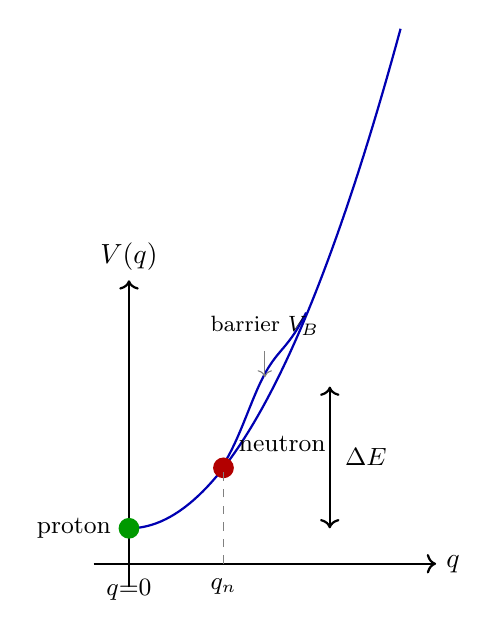
\begin{tikzpicture}[scale=1.5]
    % Axes
    \draw[thick,->] (-0.3,0) -- (2.6,0) node[right] {$q$};
    \draw[thick,->] (0,-0.2) -- (0,2.4) node[above] {$V(q)$};

    % Potential curve (base parabola)
    \draw[thick,blue!70!black,domain=0:2.3,samples=60] plot (\x, {0.3 + 0.8*\x*\x});

    % Barrier bump (schematic)
    \draw[thick,blue!70!black,domain=0.8:1.5,samples=30] plot (\x, {0.3 + 0.8*\x*\x + 0.25*exp(-18*(\x-1.15)*(\x-1.15))});

    % Proton minimum
    \fill[green!60!black] (0,0.3) circle (2.5pt);
    \node[left, xshift=-3pt, font=\small] at (0,0.3) {proton};
    \node[below, yshift=-2pt, font=\small] at (0,0) {$q{=}0$};

    % Neutron excited
    \fill[red!70!black] (0.8,0.812) circle (2.5pt);
    \node[above right, xshift=2pt, yshift=2pt, font=\small] at (0.8,0.82) {neutron};
    \draw[dashed, gray] (0.8,0) -- (0.8,0.812);
    \node[below, yshift=-2pt, font=\small] at (0.8,0) {$q_n$};

    % Energy difference arrow
    \draw[<->, thick] (1.7,0.3) -- (1.7,1.5);
    \node[right, xshift=2pt, font=\small] at (1.7,0.9) {$\Delta E$};

    % Barrier label
    \node[above, font=\footnotesize] at (1.15,1.85) {barrier $V_B$};
    \draw[->, thin, gray] (1.15,1.8) -- (1.15,1.58);
\end{tikzpicture}
\caption{\textbf{Schematic potential $V(q)$ for the junction coordinate.} The proton
sits at $q=0$ (Steiner minimum); the neutron at $q_n > 0$ (metastable excited state).
A barrier $V_B$ separates neutron from proton, determining the tunneling lifetime.}
\label{fig:n_potential}
\end{figure}

\paragraph{Baseline observable \tagBL{}.}
Experimentally, the dominant channel is:
\begin{equation}
n \to p + e^- + \bar\nu_e,
\label{eq:n_channel}
\end{equation}
with a Q-value governed by the neutron--proton mass difference:
$\Delta m_{np} = m_n - m_p \approx 1.293$ MeV \tagBL{}.

EDC does not dispute the baseline; it supplies an interface mechanism that makes
the channel structure intelligible.

% ============================================================
%  MECHANICS PICTURE
% ============================================================
\subsubsection{Mechanics Picture: Ring + 3 Springs}
\label{subsec:n_mechanics}

To build intuition for the junction dynamics, we introduce a mechanical analogy.

\begin{tcolorbox}[edcModel, title={Mechanical Analogy: Ring + 3 Springs \tagI{}/\tagP{}}]
Consider a circular ring of radius $R$ with three springs attached at angles
$\theta_1, \theta_2, \theta_3$, each pulling toward the center with spring
constant $k$. The springs represent flux-tube tensions; the ring represents a
collective constraint.

\medskip
\textbf{Interpretation:}
\begin{itemize}[nosep]
  \item Equilibrium: $\theta_1 = \theta_2 = \theta_3 = 120\degree$ (proton)
  \item Excited: angles deviate, springs store extra energy (neutron)
  \item Ring constraint couples all three modes (collective dynamics)
\end{itemize}
\end{tcolorbox}

\paragraph{Three-mode decomposition.}
The junction has three angular degrees of freedom $(\theta_1, \theta_2, \theta_3)$
subject to $\theta_1 + \theta_2 + \theta_3 = 2\pi$. This leaves two independent modes:
\begin{align}
q &= \text{(collective asymmetry)} = \frac{1}{3}|\hat{e}_1 + \hat{e}_2 + \hat{e}_3|
    \tag{radial} \\
\perp_1, \perp_2 &= \text{(transverse modes)} \tag{angular}
\end{align}
The collective coordinate $q$ measures overall departure from Steiner; the
transverse modes $\perp_{1,2}$ describe shape distortions at fixed $q$.

For slow (adiabatic) relaxation, the transverse modes equilibrate quickly, and
the effective dynamics is one-dimensional in $q$. This justifies the 1D WKB
treatment \tagI{}.

\paragraph{Linearized oscillation.}
Near the metastable neutron configuration $q = q_n$, the dynamics linearizes to:
\begin{equation}
\ddot{q} + 2\gamma \dot{q} + \omega_0^2 (q - q_n) = 0
\label{eq:n_damped_oscillator}
\end{equation}
where $\omega_0$ = natural frequency (junction stiffness) \tagP{}, and
$\gamma$ = effective damping (energy loss to brane modes) (open).

\textbf{Note:} This is a \textbf{mechanical linearization} around a geometric
minimum---not a quantum field theory oscillator. It captures the qualitative
behavior: the junction oscillates around its metastable position while losing
energy to the brane.

% ============================================================
%  PHYSICAL PROCESS NARRATIVE
% ============================================================
\subsubsection{The Mechanistic Story: The ``Film'' of Neutron Decay}
\label{subsec:n_film}

We narrate the process following the canonical \textbf{Physical Process Narrative
(PPN)} framework for energy transfer in EDC.

\begin{tcolorbox}[edcPPN, title={Physical Process Narrative (PPN): Bulk $\to$ Brane $\to$ Observer}]
\begin{enumerate}[nosep,leftmargin=*]
  \item[\textbf{(i)}] \textbf{Bulk cause (5D):} Change in bulk-core configuration
        $q(t)$ (junction displacement from Steiner) releases geometric energy
        $\Delta E \approx \Delta m_{np}c^2$.

  \item[\textbf{(ii)}] \textbf{Injection to brane:} This change pumps energy into
        brane-layer modes $\phi$ at the bulk-facing boundary via
        $\mathcal{L}_{\mathrm{int}} = g\,q(t)\,\phi(-\delta/2,t)$.

  \item[\textbf{(iii)}] \textbf{Absorption:} The brane accepts the excess energy
        from the bulk process and stores it as excitations of its degrees of
        freedom (brane-layer storage).

  \item[\textbf{(iv)}] \textbf{Dissipation/relaxation:} Within the brane-layer,
        energy redistributes across modes, loses coherence (coarse-graining/decoherence),
        and flows toward allowed output channels.

  \item[\textbf{(v)}] \textbf{Frozen projection (observer side):} The operator
        $\mathcal{P}_{\mathrm{frozen}}$ maps brane-layer excitations to observable
        3D outputs ($e^- + \bar{\nu}_e + \text{recoil}$), enforcing selection rules.

  \item[\textbf{(vi)}] \textbf{Ledger closure:} Total 5D conservation holds; the
        brane redirects energy/quantum numbers from bulk channels to observer
        channels without ``magical disappearance.''
\end{enumerate}
\end{tcolorbox}

\paragraph{Stage A: Absorption (brane charging by junction relaxation).}

A junction relaxation in the bulk-core sector induces a bulk-facing pumping into
the brane layer. In the effective brane coordinate picture, we model this as a
trajectory $q(t)$ in an effective potential $V(q)$, with instantaneous pumping
power:
\begin{equation}
\Pi_{\text{pump}}(t) \equiv -\dot{q}(t) \cdot \partial_q V(q(t)).
\label{eq:n_pump}
\end{equation}

\textbf{Interpretation} \tagDc{}: The quantity $\Pi_{\text{pump}}$ is not a new
force; it is the power delivered into the brane reservoir by the bulk-side
relaxation mechanism. When $\dot{q} < 0$ (relaxation toward $q=0$) and
$\partial_q V > 0$ (uphill from neutron side), the product is positive.

The accumulated energy delivered into the brane up to time $t$ is the charging
integral:
\begin{equation}
E_{\text{charge}}(t) \equiv \int_0^t \Pi_{\text{pump}}(t')\,dt'.
\label{eq:n_charge}
\end{equation}

\paragraph{Stage B: Dissipation (redistribution into brane-layer modes) \tagP{}.}

Once energy is deposited, it need not be immediately released. A thick brane
provides internal degrees of freedom (layer modes) into which the reservoir
energy can redistribute:
\begin{equation}
E_{\text{brane}} \;\to\; \{\phi_k\}_{\text{layer modes}}.
\label{eq:n_modes}
\end{equation}

This stage is crucial: without it, one cannot explain why the observed outputs
appear as a restricted set rather than an arbitrary energy dump.

The coupling of the junction coordinate $q(t)$ to brane-layer modes induces an
effective dissipation. Integrating out the fast brane degrees of freedom yields
a damped equation of motion \tagP{}:
\begin{equation}
\boxed{M \ddot{q} + \Gamma \dot{q} + \partial_q V(q) = 0}
\label{eq:n_damped_motion}
\end{equation}
where $M$ = effective mass (junction inertia), $\Gamma$ = effective damping
coefficient (brane-layer dissipation), and $V(q)$ = effective potential from
junction geometry (Fig.~\ref{fig:n_potential}).

\textbf{Physical interpretation of $\Gamma$} \tagP{}: The coefficient
$\Gamma$ encodes the energy transfer rate from the bulk-core junction to brane-layer
modes. $\Gamma = 0$ means no coupling (unphysical); $\Gamma > 0$ means junction
energy drains into brane modes. Note: $\Gamma$ is NOT fitted to the neutron
lifetime $\tau_n$ in this chapter. Its derivation from thick-brane microphysics
remains (open).

\paragraph{Stage C: Release (observer-facing projection into 3D outputs) \tagDc{}.}

The release stage begins when the system enters a regime where pumping becomes
negligible compared to release:
\begin{equation}
\Xi(t) \equiv \frac{\Pi_{\text{pump}}(t)}{\Pi_{\text{release}}(t)} \ll 1
\quad\text{at } t = t_*.
\label{eq:n_trigger}
\end{equation}

\textbf{Important nuance}: We do not claim that $\dot{q}(t_*) = 0$ exactly.
Rather, the interface becomes \emph{effectively frozen} at observational
resolution: the continuous pump term is negligible, and the release can be
treated as the dominant process.

The observer-facing outputs are defined by the frozen projection operator
:
\begin{equation}
\{\text{outputs}\}_{3D} = \mathcal{P}_{\text{frozen}}\big(\{\phi_k\}\big),
\qquad
\mathcal{P}_{\text{frozen}} = \mathcal{P}_{\text{energy}} \circ
\mathcal{P}_{\text{mode}} \circ \mathcal{P}_{\text{chir}}.
\label{eq:n_projection}
\end{equation}

% ============================================================
%  CANONICAL GLOSSARY BOX
% ============================================================
\begin{tcolorbox}[edcCanonical, title={Canonical Brane-Language for Neutron Decay}]
The neutron decay process involves \textbf{three conceptually distinct phases},
all part of a single energy-conserving flow:

\medskip
\textbf{(1) Absorption / Charging} (bulk $\to$ brane-layer) \tagDc{}\\
The brane \textbf{receives} energy from the relaxing bulk-core junction. This is
not ``creation''---it is \emph{transfer} governed by the coupling $\mathcal{L}_{\mathrm{int}}$.

\emph{Ledger:} $\Delta E_{\mathrm{brane}} = -\Delta E_{\mathrm{bulk}} - E_{\mathrm{other}}$

\medskip
\textbf{(2) Dissipation / Redistribution} (within brane-layer) \tagP{}\\
Internal brane-layer dynamics \textbf{redistribute} the absorbed energy into allowed
mode excitations $\{\phi_k\}$. ``Dissipation'' does \textbf{not} mean energy loss---it
means transition from coherent pumping channel to spectral mode distribution.

\emph{Mechanism:} Characterized by $\Gamma_{\mathrm{eff}}$ (effective redistribution rate).

\medskip
\textbf{(3) Release / Emission} (brane-layer $\to$ 3D observer) \tagDc{}/\tagP{}\\
The frozen projection operator $\mathcal{P}_{\mathrm{frozen}}$ \textbf{maps} brane-layer
modes to allowed 3D particle outputs. This is \emph{not} ``particle creation from
nothing''---it is a boundary projection enforcing selection rules.

\emph{Output:} $\{\phi_k\} \xrightarrow{\mathcal{P}_{\mathrm{frozen}}}
\{e^-, \bar{\nu}_e, \mathrm{recoil}, \mathrm{soft}\}_{\mathrm{3D}}$

\medskip
\hrule
\medskip
\textbf{One-liner (citable):}
\begin{quote}
\emph{``Neutron decay in EDC is bulk-core relaxation that charges the brane
(absorption), the brane redistributes energy into layer modes (dissipation),
and the observer-facing boundary projects those modes into allowed 3D particle
outputs (release).''}
\end{quote}
\end{tcolorbox}

% ============================================================
%  FROZEN PROJECTION MECHANISM
% ============================================================
\subsubsection{Frozen Projection Boundary}
\label{subsec:n_frozen}

\paragraph{One-way valve mechanism \tagDc{}/\tagP{}.}
The frozen projection boundary acts as a \textbf{one-way valve}:
\begin{itemize}[nosep]
  \item \textbf{INFLOW} (bulk $\to$ brane): spontaneously allowed
  \item \textbf{OUTFLOW} (brane $\to$ bulk): energetically/kinematically suppressed
\end{itemize}

\textbf{Physical interpretation:} The boundary condition at the observer-facing
side ``freezes'' high-energy bulk modes, preventing their re-excitation from the
3D side. This is analogous to decoherence: environmental tracing eliminates
coherent bulk superpositions.

\paragraph{Formal definition/\tagDc{}.}
Let $\phi(y, t)$ denote the brane-layer field, where $y \in [-\delta/2, +\delta/2]$
is the coordinate across the brane thickness. The \textbf{frozen projection operator}
$\mathcal{P}_{\mathrm{frozen}}$ maps brane-layer excitations at the observer-facing
boundary to observable 3D particle states:
\begin{equation}
\boxed{\mathcal{P}_{\mathrm{frozen}}: \quad
\phi\bigl(y = +\tfrac{\delta}{2}, t\bigr) \;\longmapsto\;
\{e^-, e^+, \nu_e, \bar{\nu}_e, \gamma, \ldots\}_{\mathrm{3D}}}
\label{eq:n_frozen_projection}
\end{equation}

The operator acts as follows:
\begin{enumerate}[nosep]
  \item Identifies modes satisfying the frozen criterion ($\hbar\omega \gg E_{\mathrm{env}}$)
  \item Projects these onto mass-shell particle states
  \item Enforces selection rules (charge, lepton number, energy threshold)
\end{enumerate}

\paragraph{Frozen criterion/\tagDc{}.}
A brane-layer mode with characteristic frequency $\omega$ is \textbf{frozen}
(appears as a fixed particle rather than a fluctuating field) when:
\begin{equation}
\boxed{\hbar\omega \gg E_{\mathrm{env}}}
\label{eq:n_frozen_criterion}
\end{equation}
where $E_{\mathrm{env}}$ is the typical environmental energy scale on the 3D side.
For neutron decay at room temperature ($E_{\mathrm{env}} \sim k_B T \sim 0.025$ eV),
all decay products ($e^-$, $\bar{\nu}_e$ with energies $\sim$ keV--MeV) satisfy
$\hbar\omega \gg E_{\mathrm{env}}$ and thus appear as stable particles.

\paragraph{Irreversibility \tagDc{}/\tagP{}.}
The frozen projection is effectively \textbf{irreversible}: once energy passes
through $\mathcal{P}_{\mathrm{frozen}}$ and materializes as 3D particles, it
cannot spontaneously return to bulk-core excitations. This explains why neutron
decay is observed but ``inverse beta decay'' ($p + e^- + \bar{\nu}_e \to n$)
requires external energy input.

% ============================================================
%  SELECTION RULES
% ============================================================
\subsubsection{Why the Electron Channel Is Allowed but the Muon Channel Is Not}
\label{subsec:n_selection}

A common confusion is to phrase this as ``EDC forbids the muon channel.'' The
correct, book-level statement is purely kinematic and belongs to
$\mathcal{P}_{\text{energy}}$.

\paragraph{Baseline kinematic gate \tagBL{}.}
For $\beta$-decay, the available energy budget is set by:
\begin{equation}
Q_\beta(\ell) \approx \Delta m_{np} - m_\ell - m_\nu \approx \Delta m_{np} - m_\ell,
\label{eq:n_Q_beta}
\end{equation}
where neutrino masses are negligible at this scale.

\paragraph{Electron channel.}
For $\ell = e$ one has $m_e \approx 0.511$ MeV \tagBL{}, hence $Q_\beta(e) > 0$,
so phase space exists and the channel is kinematically open:
\begin{equation}
Q_\beta(e) \approx 1.293 - 0.511 = 0.782~\text{MeV} > 0.
\label{eq:n_Qbeta_electron}
\end{equation}

\paragraph{Muon channel.}
For $\ell = \mu$ one has $m_\mu \approx 105.7$ MeV \tagBL{}, hence
$Q_\beta(\mu) < 0$:
\begin{equation}
Q_\beta(\mu) \approx 1.293 - 105.7 \approx -104.4~\text{MeV} < 0,
\label{eq:n_Qbeta_muon}
\end{equation}
meaning there is \emph{no kinematically allowed phase space} for
$n \to p + \mu^- + \bar\nu_\mu$ at rest.

\begin{tcolorbox}[edcGuardrail, title={Q-Gate Selection Rule}]
The ``muon channel'' is rejected not by metaphysical prohibition, but because
$\mathcal{P}_{\text{energy}}$ yields zero support:
\begin{equation}
\mathcal{P}_{\text{energy}}: \quad
\text{channel allowed} \iff Q_\beta(\ell) > 0.
\label{eq:n_Penergy_gate}
\end{equation}
This is a kinematic fact \tagBL{}, not an EDC-specific assumption.
\end{tcolorbox}

\paragraph{What ``forbids'' means physically.}
The word ``forbids'' is not metaphysical; it has a precise kinematic meaning:

\begin{itemize}[nosep]
  \item \textbf{Energy budget}: The neutron at rest has total energy $m_n c^2$.
        After decay, the products must share this energy (minus binding).
  \item \textbf{Rest mass floor}: The \emph{minimum} energy required to produce
        $p + \mu^- + \bar\nu_\mu$ is their combined rest masses:
        $m_p + m_\mu + m_\nu \approx 938.3 + 105.7 + 0 = 1044$ MeV.
  \item \textbf{Comparison}: But $m_n c^2 \approx 939.6$ MeV $<$ 1044 MeV.
  \item \textbf{Conclusion}: There is \emph{no real final state} satisfying
        energy-momentum conservation. The muon channel is kinematically closed.
\end{itemize}

\noindent
A muon \emph{can} appear as a \textbf{virtual particle} in loop diagrams (off-shell),
but it cannot emerge as a real, on-shell particle in the final state without an
external energy source. This is standard relativistic kinematics \tagBL{}, not an
EDC claim.

\paragraph{EDC interpretation.}
This is exactly what we want from the pipeline language: one can separate
\emph{what is purely kinematic} (baseline gating) from \emph{what is mechanistic}
(how the brane actually processes and projects the allowed energy into specific
outputs). In neutron decay, $\mathcal{P}_{\text{energy}}$ restricts us to the
electron sector; the remaining question is then: \emph{given that the electron
channel is open, what interface mechanism produces the observed
$\{e^-, \bar\nu\}$ outputs?}

\paragraph{Selection rules summary \tagDc{}.}
The frozen boundary imposes selection rules on which decay products can emerge:
\begin{enumerate}[nosep]
  \item \textbf{Charge conservation:} $Q_{\text{in}} = Q_{\text{out}}$
        (neutron: $0 \to +1 + (-1) + 0$)
  \item \textbf{Lepton number:} $L_e: 0 \to 0 + 1 + (-1) = 0$ (\checkmark)
  \item \textbf{Energy threshold:} $\Delta E > m_e c^2$ required for electron emission
  \item \textbf{Momentum matching:} recoil absorbed by proton
\end{enumerate}

\textbf{Suppressed channels:}
\begin{itemize}[nosep]
  \item $n \to p + \mu^- + \bar{\nu}_\mu$: Forbidden by $m_\mu > \Delta E$
  \item $n \to p + \gamma$: Suppressed (no photon channel in lowest-order weak)
  \item $n \to p + e^- + e^+ + \nu_e + \bar{\nu}_e$: Phase space suppressed
\end{itemize}

\paragraph{V--A structure \tagBL{}.}
The $V-A$ (vector minus axial-vector) structure of weak interactions is
\textbf{not derived here}---it is input from Standard Model phenomenology.
EDC provides the energy release mechanism; the detailed interaction vertex is
inherited.

% ============================================================
%  ENERGY BOOKKEEPING
% ============================================================
\subsubsection{Ledger Closure for Neutron Decay}
\label{subsec:n_ledger}

The neutron case forces discipline on bookkeeping. The brane reservoir must close
its ledger: the energy deposited by junction relaxation must appear as observable
kinetic energies plus any additional channels consistent with conservation.

\paragraph{Charging ledger \tagDc{}.}
During the charging phase, energy conservation requires:
\begin{equation}
\boxed{\Delta E_{\mathrm{brane}} = -\Delta E_{\mathrm{bulk}} - E_{\mathrm{other}}}
\label{eq:n_charging_ledger}
\end{equation}
where:
\begin{itemize}[nosep]
  \item $\Delta E_{\mathrm{bulk}} = E(q{=}0) - E(q{=}q_n) < 0$ (bulk loses geometric
        excitation energy)
  \item $\Delta E_{\mathrm{brane}} > 0$ (brane gains stored energy)
\end{itemize}

The residual term $E_{\mathrm{other}}$ decomposes as:
\begin{equation}
E_{\mathrm{other}} = E_{\mathrm{recoil}} + E_{\mathrm{soft}} + E_{\mathrm{bulk\,residual}}
\label{eq:n_e_other}
\end{equation}
\begin{itemize}[nosep]
  \item $E_{\mathrm{recoil}}$: 3D momentum balance (proton recoil) \tagDc{}
  \item $E_{\mathrm{soft}}$: low-energy brane modes, soft photons/phonons \tagP{}
  \item $E_{\mathrm{bulk\,residual}}$: any energy remaining in bulk (if leakage
        permitted) \tagP{}
\end{itemize}

\paragraph{Schematic ledger identity/\tagDc{}.}
\begin{equation}
\Delta E_{\text{available}} = K_p + K_e + K_{\bar\nu} + E_{\text{other}},
\label{eq:n_ledger}
\end{equation}
where:
\begin{itemize}[nosep]
  \item $\Delta E_{\text{available}}$ is the energy budget ($\sim Q_\beta$),
  \item $K_p, K_e, K_{\bar\nu}$ are the kinetic energies of the outputs,
  \item $E_{\text{other}} = E_{\text{recoil}} + E_{\text{soft}} + E_{\text{bulk,res}}$
        collects subleading channels/(open).
\end{itemize}

For neutron decay: $|\Delta E_{\mathrm{bulk}}| \approx \Delta m_{np} c^2 \approx
1.293$ MeV \tagBL{} (PDG neutron--proton mass difference).

% --- ENERGY BOOKKEEPING TABLE ---
\begin{table}[ht]
\centering
\caption{Energy Bookkeeping for Neutron $\beta^-$ Decay \tagDc{}/\tagP{}}
\label{tab:n_energy_bookkeeping}
\small
\begin{tabular}{@{}lllll@{}}
\toprule
\textbf{Term} & \textbf{Meaning} & \textbf{Tag} & \textbf{Units} & \textbf{Location} \\
\midrule
$\Delta E_{\mathrm{bulk}}$ & Junction relaxation energy & \tagDc{} & MeV & Bulk-core \\
$\Delta E_{\mathrm{brane}}$ & Stored brane energy (charging) & \tagDc{} & MeV & Brane-layer \\
$E_e$ & Electron kinetic + rest mass & \tagBL{} & MeV & 3D output \\
$E_{\bar{\nu}}$ & Antineutrino energy & \tagBL{} & MeV & 3D output \\
$E_{\mathrm{recoil}}$ & Proton recoil & \tagDc{} & keV & 3D output \\
$E_{\mathrm{soft}}$ & Soft photons/phonons & \tagP{} & $\ll$ keV & Brane/3D \\
$E_{\mathrm{bulk\,res.}}$ & Bulk residual (if any) & \tagP{} & --- & Bulk \\
\midrule
\multicolumn{5}{@{}l@{}}{\textbf{Conservation check:} $|\Delta E_{\mathrm{bulk}}|
= \Delta E_{\mathrm{brane}} + E_{\mathrm{other}}$} \\
\multicolumn{5}{@{}l@{}}{\textbf{Release check:} $\Delta E_{\mathrm{brane}}
= E_e + E_{\bar{\nu}} + E_{\mathrm{recoil}} + E_{\mathrm{soft}}$} \\
\midrule
\multicolumn{5}{@{}l@{}}{\textbf{Numerical benchmark} \tagBL{}:
$|\Delta E_{\mathrm{bulk}}| \approx 1.293$ MeV (PDG)} \\
\bottomrule
\end{tabular}
\end{table}

% ============================================================
%  PROCESS DIAGRAM
% ============================================================
\subsubsection{Process Diagram: Neutron Decay}
\label{subsec:n_diagram}

\begin{center}
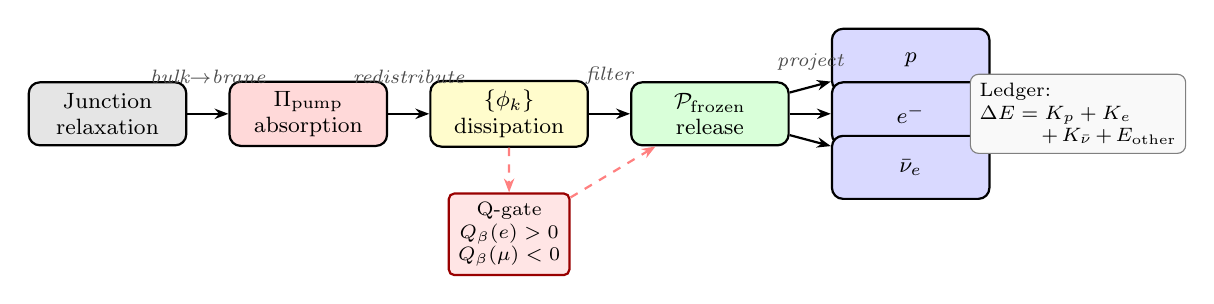
\begin{tikzpicture}[
  scale=0.85,
  box/.style={rectangle, rounded corners=4pt, minimum width=2cm, minimum height=0.8cm,
              draw=black, thick, font=\footnotesize, align=center},
  gate/.style={rectangle, rounded corners=2pt, minimum width=1.5cm, minimum height=0.6cm,
               draw=red!60!black, thick, fill=red!10, font=\scriptsize, align=center},
  arrow/.style={-{Stealth[length=5pt]}, thick},
  label/.style={font=\scriptsize\itshape, text=gray!60!black}
]

% Stage boxes
\node[box, fill=gray!20] (junction) at (0,0) {Junction\\relaxation};
\node[box, fill=red!15] (pump) at (3,0) {$\Pi_{\text{pump}}$\\absorption};
\node[box, fill=yellow!20] (modes) at (6,0) {$\{\phi_k\}$\\dissipation};
\node[box, fill=green!15] (project) at (9,0) {$\mathcal{P}_{\text{frozen}}$\\release};

% Q-gate
\node[gate] (qgate) at (6,-1.8) {Q-gate\\$Q_\beta(e)>0$\\$Q_\beta(\mu)<0$};

% Outputs
\node[box, fill=blue!15] (p) at (12,0.8) {$p$};
\node[box, fill=blue!15] (e) at (12,0) {$e^-$};
\node[box, fill=blue!15] (nu) at (12,-0.8) {$\bar\nu_e$};

% Arrows
\draw[arrow] (junction) -- (pump);
\draw[arrow] (pump) -- (modes);
\draw[arrow] (modes) -- (project);
\draw[arrow] (project) -- (p);
\draw[arrow] (project) -- (e);
\draw[arrow] (project) -- (nu);
\draw[arrow, dashed, red!50] (modes) -- (qgate);
\draw[arrow, dashed, red!50] (qgate) -- (project);

% Labels
\node[label, above] at (1.5,0.3) {bulk$\to$brane};
\node[label, above] at (4.5,0.3) {redistribute};
\node[label, above] at (7.5,0.3) {filter};
\node[label, above] at (10.5,0.5) {project};

% Ledger box
\node[rectangle, draw=gray, rounded corners=3pt, fill=gray!5,
      font=\scriptsize, align=left, text width=2.5cm] at (14.5,0)
  {Ledger:\\$\Delta E = K_p + K_e$\\$\phantom{\Delta E =} + K_{\bar\nu} + E_{\text{other}}$};

\end{tikzpicture}
\end{center}

\paragraph{Decay process mapping \tagDc{}.}

\begin{center}
\begin{tabular}{p{4cm}cp{5cm}}
\toprule
\textbf{5D (Cause)} & & \textbf{3D (Effect)} \\
\midrule
Junction relaxes: $q_n \to 0$ & $\Rightarrow$ & $n \to p$ \\
Energy pumped to brane: $\Delta E \approx 1.293$ MeV & $\Rightarrow$ & Kinetic energy of products \\
Brane modes organize via selection rules & $\Rightarrow$ & $e^- + \bar{\nu}_e$ emission \\
\bottomrule
\end{tabular}
\end{center}

% ============================================================
%  OBSERVABLE BENCHMARKS
% ============================================================
\subsubsection{Observable Benchmarks (No Fitting)}
\label{subsec:n_benchmarks}

This section lists observable quantities and their status in the EDC neutron model.
\textbf{No parameters are fitted in this case study.}

\begin{center}
\begin{tabular}{lccl}
\toprule
\textbf{Observable} & \textbf{Value} & \textbf{Status} & \textbf{Notes} \\
\midrule
Neutron lifetime $\tau_n$ & $879.4 \pm 0.6$ s & \tagBL{} & PDG 2024 \\
Mass difference $\Delta m_{np}$ & 1.293 MeV & \tagBL{} & CODATA \\
$Q$-value ($n \to p + e + \bar{\nu}$) & 0.782 MeV & \tagBL{} & Kinematic endpoint \\
Proton recoil & $\sim$ keV & \tagBL{} & Small due to mass ratio \\
\midrule
$\Delta m_{np}$ from $\mathbb{Z}_6$ breaking & 1.30 MeV & \tagDc{} & From geometry \\
$q_n \approx 1/3$ & identified & \tagI{} & Half-Steiner (OPR-24) \\
Barrier height $V_B$ & $\sim 2.6$ MeV & \tagCal{} & Fitted to $\tau_n$ (OPR-23) \\
\bottomrule
\end{tabular}
\end{center}

\textbf{Important \tagCal{}:} The neutron lifetime $\tau_n \approx 879$ s can be
reproduced via WKB tunneling through a barrier $V_B$. However, $V_B$ is
\textbf{calibrated} to match $\tau_n$, not derived from first principles. A
first-principles derivation of $V_B$ (or equivalently, the attempt frequency
$\Gamma_0$) remains (open).

% ============================================================
%  OPEN PROBLEMS
% ============================================================
\subsubsection{Open Problems for the Neutron Case}
\label{subsec:n_open}

\begin{enumerate}[nosep]
  \item \textbf{Derive $V_B$ from 5D action} (open) (OPR-23): Current status is $V_B
        \approx 2.6$ MeV (calibrated). Goal: show $V_B$ emerges from junction
        geometry + brane tension. Would upgrade $\tau_n$ from \tagCal{} to \tagDer{}.

  \item \textbf{WKB--Damping Bridge} (open): The WKB treatment uses tunneling
        through $V(q)$; this section uses damped oscillator + pumping. Goal: show
        equivalence in appropriate limits.

  \item \textbf{Thick-brane coupling $g$} (open): Postulated in
        $\mathcal{L}_{\mathrm{int}} = g\,q(t)\,\phi$. Need: derive from 5D action
        or constrain from observables.

  \item \textbf{Precise value of $q_n$} \tagI{} (OPR-24): Currently $q_n \approx
        1/3$ from $\mathbb{Z}_6$ symmetry arguments. Need: reconcile or derive from
        first principles.
\end{enumerate}

% ============================================================
%  FALSIFIABILITY HOOKS
% ============================================================
\subsubsection{Falsifiability Hooks}
\label{subsec:n_falsifiability}

\begin{tcolorbox}[falsifiability]
The neutron mechanistic story can be wrong. The most direct falsifiability hooks are:
\begin{itemize}[nosep]
  \item If the mechanism predicts additional leading-order outputs beyond
        $\{p, e^-, \bar\nu_e\}$ in the neutron Q-window, it fails.
  \item If $\mathcal{P}_{\text{energy}}$ gating is not respected (i.e., if the
        model leaks into the $\mu$ channel without external energy), it fails.
  \item If the ledger cannot be closed without hidden tuning (i.e., energy
        ``disappears'' without accounted bins), it fails.
  \item If the trigger condition requires an ad hoc fitted parameter rather
        than a regime statement, it fails.
  \item If $E_{\mathrm{other}}$ lacks structure (e.g., all energy goes to
        $e^- + \bar{\nu}$ with no recoil accounting), the ledger picture must
        be revised.
  \item If the frozen projection cannot exclude forbidden channels (e.g.,
        $\gamma + p$, $\mu^- + \bar{\nu}_\mu + p$), the weak-sector narrative fails.
\end{itemize}
\end{tcolorbox}

\begin{tcolorbox}[edcGuardrail, title={Epistemic Guardrail: Observation vs.\ Explanation}]
\textbf{(1) Baseline observable} \tagBL{}:\\
The neutron lifetime $\tau_n = 878.4 \pm 0.5\,\mathrm{s}$ is an \textbf{empirical
fact} measured in 3D. It is \textbf{not} a parameter we choose or fit in this chapter.

\medskip
\textbf{$\tau_n$ is not a control knob:} We treat $\tau_n$ as a \textbf{benchmark}
\tagBL{}, not as a tuning target. Any mapping $\tau_n \leftrightarrow
(\Gamma, g, \delta, \ldots)$ is deferred to (open) work.

\medskip
\textbf{(2) Theoretical explanation} \tagP{}/\tagDc{}:\\
The EDC claim is that $\tau_n$ is \textbf{explained} (not tuned) by the bulk-to-brane
relaxation mechanism.

\medskip
\textbf{(3) Placeholder parameters} (open):\\
Any effective parameters introduced ($\Gamma$, $g$, $\delta$, $\Pi_{\mathrm{pump}}$,
etc.) are \textbf{microphysical placeholders} until derived from the brane model.
\end{tcolorbox}

% ==============================================================================
% STOPLIGHT VERDICT (2026-01-29)
% ==============================================================================
\subsubsection{Stoplight Verdict}
\label{subsec:neutron_stoplight}

\begin{tcolorbox}[colback=yellow!10!white, colframe=orange!60!black,
    title=\textbf{Case Neutron: Stoplight Verdict}]

\begin{center}
\begin{tabular}{@{}lll@{}}
\toprule
\textbf{Claim} & \textbf{Status} & \textbf{Tag} \\
\midrule
Bulk-core junction ontology & \textcolor{YellowOrange}{\textbf{YELLOW}} & \tagP{} \\
Channel selection ($e^-$ only) & \textcolor{OliveGreen}{\textbf{GREEN}} & \tagDc{} \\
$\tau_n$ order of magnitude & \textcolor{YellowOrange}{\textbf{YELLOW}} & \tagDc{}/\tagCal{} \\
Frozen projection mechanism & \textcolor{YellowOrange}{\textbf{YELLOW}} & \tagP{}/\tagDc{} \\
\bottomrule
\end{tabular}
\end{center}

\textbf{Overall: YELLOW} --- Mechanism identified; quantitative closure requires
BVP mode profiles (OPR-21) and first-principles $\tau_n$ derivation.

\textbf{Blockers:}
\begin{itemize}[nosep]
\item Junction dislocation dynamics from 5D action
\item Prefactor $A$ derivation (currently \tagCal{})
\item $L_0/\delta$ ratio from microphysics
\end{itemize}

See \S\ref{sec:gate_registry} for consolidated gate registry.
\end{tcolorbox}


% ==============================================================================
% Case Study II: Muon Decay as Brane-Dominant Mode Relaxation
% ==============================================================================

\subsection{Muon Decay: Brane-Dominant Mode Relaxation}
\label{sec:muon_story}

Unlike the neutron, the muon does not require a bulk-core junction ontology.
In the EDC Weak Program, the muon is treated as a \emph{brane-dominant excitation}:
a localized brane-layer defect/mode that stores energy primarily in the brane subsystem,
and relaxes via the same three-phase pipeline (absorption $\to$ dissipation $\to$ release),
but with the \emph{bulk trigger removed at leading order}.

\subsubsection{Ontology and What Makes the Muon a Clean Test}

\begin{edcDefinitionBox}{Muon as a brane-dominant excitation}{[Def]/[P]}
We model the muon as an excitation $\Psi_\mu$ in the brane-layer mode spectrum, with dominant
energy support in the brane (not in the bulk-core junction). The decay is the relaxation
$\Psi_\mu \to \Psi_e$ through brane-layer redistribution and frozen projection into allowed outputs.
\end{edcDefinitionBox}

This makes $\mu$-decay a clean test of the brane mechanism because:
\begin{enumerate}[nosep]
  \item[(i)] there is no ambiguity of bulk-core topology,
  \item[(ii)] the output channel is experimentally sharp, and
  \item[(iii)] the chirality structure is a strong selection signature.
\end{enumerate}

\paragraph{Baseline observable.}
Experimentally the dominant decay is \tagBL{}:
\begin{equation}
\mu^- \to e^- + \bar\nu_e + \nu_\mu,
\label{eq:mu_decay_channel_story}
\end{equation}
with an almost purely leptonic final state and lifetime $\tau_\mu \approx 2.197 \times 10^{-6}$ s \tagBL{}.

\subsubsection{Pipeline for Muon Decay}

We reuse the unified pipeline:
\begin{equation}
\label{eq:mu_pipeline}
\Psi_\mu
\;\Rightarrow\;
E_{\mathrm{brane}} \text{ (stored)}
\;\Rightarrow\;
\Gamma_{\mathrm{eff}} \text{ (redistribution)}
\;\Rightarrow\;
\mathcal{P}_{\mathrm{frozen}} \text{ (3D outputs)}.
\end{equation}

\paragraph{Absorption / charging \tagDc{}.}
For a brane-dominant excitation, the ``absorption'' stage is not pumping from bulk,
but simply the existence of stored brane energy in the excited configuration:
\begin{equation}
\label{eq:mu_brane_energy}
E_{\mathrm{brane}}(t_0) \approx m_\mu c^2 \approx 105.7~\text{MeV} \quad \text{\tagBL{}},
\end{equation}
up to small corrections (soft, recoil, residual leakage) \tagOpen{}.

\paragraph{Dissipation (mode redistribution) \tagDc{}/\tagP{}.}
We use the same phenomenological release-rate definition:
\begin{equation}
\label{eq:mu_release_power}
\Pi_{\mathrm{release}}(t) \equiv \Gamma_{\mathrm{eff}}\,E_{\mathrm{brane}}(t),
\end{equation}
where $\Gamma_{\mathrm{eff}}$ must ultimately be derived from thick-brane microphysics \tagOpen{}.

\paragraph{Release map (allowed outputs) \tagDef{}/\tagDc{}.}
The frozen projection maps brane-layer modes into allowed 3D outputs:
\begin{equation}
\label{eq:mu_release}
E_{\mathrm{brane}}
\;\xrightarrow{\;\mathcal{P}_{\mathrm{frozen}}\;}
e^- + \bar\nu_e + \nu_\mu + \text{(soft/recoil)}.
\end{equation}

\subsubsection{Chiral Filter as Boundary Projection, Not a Fundamental Vertex}

A key empirical signature is the V--A chirality structure of weak outputs \tagBL{}.
In EDC we do not postulate a fundamental 3D ``weak vertex''.
Instead we hypothesize that chirality selection arises from a boundary/projection operator:
\begin{equation}
\label{eq:Pfrozen_factorization_mu}
\mathcal{P}_{\mathrm{frozen}}
=
\mathcal{P}_{\mathrm{energy}}\circ
\mathcal{P}_{\mathrm{mode}}\circ
\mathcal{P}_{\mathrm{chir}}.
\end{equation}

\begin{tcolorbox}[mechanism, title={Chirality as Boundary Phenomenon}]
\textbf{Claim} \tagP{}/\tagOpen{}: The observed V--A structure is consistent with
a boundary projection that selects allowed helicity/chirality outputs.
The operator $\mathcal{P}_{\mathrm{chir}}$ is an operator-level mechanism whose explicit derivation
requires the thick-brane boundary conditions (see \S\ref{sec:case_neutrino}).
\end{tcolorbox}

\subsubsection{Muon Ledger Closure}

\begin{edcLedgerBox}{Muon decay bookkeeping}{[Dc]}
\begin{equation}
\label{eq:mu_ledger}
m_\mu c^2
=
E_{e^-}+E_{\bar\nu_e}+E_{\nu_\mu}
+E_{\mathrm{recoil}}+E_{\mathrm{soft}}+E_{\mathrm{bulk,res}}.
\end{equation}
The role of the neutrino sector is not optional: it carries ledger-consistent energy/momentum
in a way compatible with chirality selection.
\end{edcLedgerBox}

\subsubsection{Process Diagram: Muon Decay}

\begin{figure}[ht]
\centering
% figures/fig_muon_process_pipeline.tex
% Muon decay process pipeline diagram (brane-dominant)
\begin{tikzpicture}[scale=0.90, transform shape]

% Load styles

% ─────────────────────────────────────────────────────────────────────────────
% Background regions (no bulk needed for brane-dominant)
% ─────────────────────────────────────────────────────────────────────────────
\fill[blue!8] (-5.2,0.4) rectangle (5.5,2.0);
\fill[green!8] (-5.2,-1.0) rectangle (5.5,0.4);

% Region labels
\node[font=\scriptsize, blue!50!black] at (-4.5,1.7) {Thick brane layer};
\node[font=\scriptsize, green!50!black] at (-4.5,0.1) {3D outputs};

% ─────────────────────────────────────────────────────────────────────────────
% Brane layer nodes
% ─────────────────────────────────────────────────────────────────────────────
\node[brane box, text width=2.6cm] (mu) at (-3.2,1.2)
  {Muon $\Psi_\mu$\\{\tiny brane-dominant}};

\node[brane box, text width=2.6cm] (diss) at (0.3,1.2)
  {Dissipation\\{\tiny $\Gamma_{\mathrm{eff}} E_{\mathrm{brane}}$}};

\node[gate box, text width=2.4cm, minimum height=0.8cm] (frozen) at (3.5,1.2)
  {$\mathcal{P}_{\mathrm{frozen}}$\\{\tiny release gate}};

% ─────────────────────────────────────────────────────────────────────────────
% Output layer nodes
% ─────────────────────────────────────────────────────────────────────────────
\node[output box, text width=1.6cm] (eout) at (1.0,-0.3)
  {$e^-$};

\node[output box, text width=1.6cm] (nue) at (2.8,-0.3)
  {$\bar\nu_e$};

\node[output box, text width=1.6cm] (numu) at (4.6,-0.3)
  {$\nu_\mu$};

% ─────────────────────────────────────────────────────────────────────────────
% Arrows
% ─────────────────────────────────────────────────────────────────────────────
\draw[edc flow] (mu) -- (diss);
\draw[edc flow] (diss) -- (frozen);

% Release to outputs
\draw[edc arrow] (frozen.south) -- ++(0,-0.25) -| (eout.north);
\draw[edc arrow] (frozen.south) -- ++(0,-0.25) -| (nue.north);
\draw[edc arrow] (frozen.south) -- ++(0,-0.25) -| (numu.north);

% ─────────────────────────────────────────────────────────────────────────────
% Annotations
% ─────────────────────────────────────────────────────────────────────────────

% Chiral filter annotation
\node[rectangle, draw=purple!40, fill=purple!5, rounded corners=2pt,
      font=\tiny, align=center, text width=4.5cm] at (-0.5,0.0)
  {$\mathcal{P}_{\mathrm{frozen}} = \mathcal{P}_{\mathrm{energy}} \circ \mathcal{P}_{\mathrm{mode}} \circ \mathcal{P}_{\mathrm{chir}}$\\
   V--A selection via boundary projection};

% No bulk trigger note
\node[rectangle, draw=gray!40, fill=gray!5, rounded corners=2pt,
      font=\tiny, align=center, text width=2.8cm] at (-3.2,0.0)
  {No bulk trigger\\(clean brane test)};

\end{tikzpicture}

\caption{\textbf{Muon decay in EDC as brane-dominant relaxation.}
Stored brane energy redistributes (dissipation) and is released via frozen projection
into allowed outputs, with chirality selection implemented as a boundary operator.
Unlike neutron decay, there is no bulk trigger---the muon is a clean test of the
brane-layer mechanism.}
\label{fig:muon_process_pipeline}
\end{figure}

\subsubsection{Why Muon Is a Clean Universality Test}

The muon decay channel tests whether:
\begin{itemize}[nosep]
  \item The same $\mathcal{P}_{\mathrm{frozen}}$ operator applies to brane-dominant excitations
        (not just bulk-core junctions)
  \item The chirality filter produces V--A structure without vertex tuning
  \item Ledger closure works for purely brane-layer relaxation
\end{itemize}

If these conditions hold, the weak-sector brane interface is a \emph{universal mechanism},
not a special case of neutron physics.

\subsubsection{Falsifiability Hooks}

\begin{tcolorbox}[falsifiability]
\begin{itemize}[nosep]
  \item If the mechanism predicts a dominant 2-body channel ($\mu \to e\gamma$) inconsistent with
        observed spectrum, it fails.
  \item If $\mathcal{P}_{\mathrm{chir}}$ cannot be realized as a boundary operator
        without tuning, the proposed interpretation weakens.
  \item If ledger closure requires hidden sinks not accounted by $E_{\mathrm{other}}$,
        it fails.
  \item If the muon lifetime cannot be connected to $\Gamma_{\mathrm{eff}}$ from
        brane microphysics, the quantitative program is incomplete \tagOpen{}.
\end{itemize}
\end{tcolorbox}


% ==============================================================================
% Subsection: Tau Decay (part of Section 1.7: Charged Leptons)
% ==============================================================================

\subsection{Tau Decay: Higher-Mode Brane Excitation}
\label{subsec:tau_story}
\label{sec:case_tau}  % alias for cross-references

% --- AT-A-GLANCE BOX (KB-CANON-002) ---
\begin{edcAtAGlance}{Tau Decay}
  \edcBaseline{
    Decay: Multiple channels with $\tau_\tau = 2.903 \times 10^{-13}$ s\\
    Leptonic: $\tau \to e\nu\bar\nu$ (17.8\%) and $\tau \to \mu\nu\bar\nu$ (17.4\%)\\
    Hadronic: $\tau \to$ hadrons + $\nu_\tau$ (64.8\% total)\\
    Energy: $m_\tau c^2 = 1777$ MeV (heaviest lepton)
  }
  \edcEDCView{
    Tau = higher-mode brane excitation (same ontology as muon)\\
    Larger energy budget opens hadronic channels via $\mathcal{P}_{\mathrm{energy}}$ threshold\\
    Same pipeline: stored brane energy $\to$ redistribution $\to$ frozen projection\\
    No new mechanism required---only higher mode number
  }
  \edcKeyInsight{
    The tau is the cleanest universality test: if the same absorption--dissipation--release
    mechanism works for both $\mu$ and $\tau$ without new ingredients, the weak-sector
    brane interface is truly universal, not specific to any single particle.
  }
  \edcFalsifiable{
    \textbullet\ If tau requires different ontological category than muon\\
    \textbullet\ If same $\mathcal{P}_{\mathrm{chir}}$ cannot apply without channel-specific tuning\\
    \textbullet\ If $\tau/\mu$ lifetime ratio contradicts mode-energy interpretation
  }
\end{edcAtAGlance}

\medskip

% ==============================================================================
% MOTIVATION: WHY TAU AFTER MUON?
% ==============================================================================

\subsubsection{Motivation: Why Tau After Muon?}

\begin{tcolorbox}[edcCornerstone, title=\textbf{Cornerstone: Tau as Mode-Spectrum Test}]
The tau lepton ($\tau^-$) is the heaviest charged lepton, with
$m_\tau \approx 1777$~MeV \tagBL{}. If the thick-brane
framework applies to muon decay (\S\ref{subsec:muon_story}), it must also accommodate
tau decay without introducing new mechanisms. The tau provides a
\emph{mode-spectrum test}: same brane-dominant ontology, different
mass/energy scale.
\end{tcolorbox}

The EDC weak-interaction program now has:
\begin{itemize}[nosep]
    \item \textbf{Neutron} (\S\ref{sec:case_neutron}): Bulk-core junction decay
    \item \textbf{Muon} (\S\ref{subsec:muon_story}): Brane-dominant leptonic decay
    \item \textbf{Tau} (this section): Heavier brane-dominant decay
\end{itemize}

If the same pipeline works for both $\mu$ and $\tau$, this validates the
\emph{brane-dominant excitation} hypothesis across the charged lepton
spectrum. The tau's larger mass probes a different region of the
brane-layer mode spectrum.

\paragraph{Scope limitation.}
This case study addresses \textbf{leptonic tau decays} primarily:
\begin{itemize}[nosep]
    \item $\tau^- \to e^- + \bar{\nu}_e + \nu_\tau$ \quad (electronic channel)
    \item $\tau^- \to \mu^- + \bar{\nu}_\mu + \nu_\tau$ \quad (muonic channel)
\end{itemize}
Hadronic tau decays (e.g., $\tau \to \pi\nu$, $\tau \to \rho\nu$) are
discussed as threshold-gated extensions (open). Full pion ontology is developed
in \S\ref{sec:case_pion}.

% ==============================================================================
% TAU ONTOLOGY
% ==============================================================================

\subsubsection{Tau Ontology: Brane-Dominant Higher Mode}

The tau is treated as the same ontological class as the muon: a brane-dominant excitation,
but at higher energy in the brane mode spectrum.

\begin{edcPostulateBox}{Tau Ontology}{[P]}
The tau lepton $\tau^-$ is a \emph{brane-dominant excitation} with a
higher mode index than the muon. Its primary degrees of freedom reside
within the brane layer, not in the bulk-core.
\end{edcPostulateBox}

\textbf{Physical Narration:}
\begin{enumerate}[nosep]
    \item \textbf{5D cause:} The tau occupies a higher-energy eigenmode of the
          brane-layer spectrum compared to the muon.
    \item \textbf{Brane response:} This mode is unstable; it can decay into
          lower-mass modes (electrons, muons, neutrinos, hadrons) via internal
          redistribution.
    \item \textbf{3D output:} The frozen projection maps allowed mode
          combinations to observable particles.
\end{enumerate}

% ==============================================================================
% MODE INDEX DEFINITION
% ==============================================================================

\subsubsection{Mode Index Hypothesis}

\begin{edcDefinitionBox}{Mode Index}{[P]}
We associate each charged lepton with a \emph{mode index} $n_\ell$
characterizing its position in the brane-layer spectrum:
\[
    n_e < n_\mu < n_\tau
\]
Higher mode index corresponds to higher mass and shorter lifetime
(greater instability).
\end{edcDefinitionBox}

\textbf{Note:} The mode index is a qualitative ordering \tagP{}.
We do not claim to derive $n_\ell$ values or the precise relationship
$m_\ell(n_\ell)$ from first principles.

% ==============================================================================
% MODE SPECTRUM FIGURE
% ==============================================================================

\begin{figure}[htbp]
\centering
\begin{tikzpicture}[scale=0.85]
    % Background regions
    \fill[bulk region] (-4.5,-2.5) rectangle (-1.5,2.5);
    \fill[brane region] (-1.5,-2.5) rectangle (1.5,2.5);
    \fill[observer region] (1.5,-2.5) rectangle (4.5,2.5);

    % Labels
    \node[section label] at (-3,2.9) {\textbf{Bulk-Core}};
    \node[section label] at (0,2.9) {\textbf{Brane-Layer}};
    \node[section label] at (3,2.9) {\textbf{3D Outputs}};

    % Boundaries
    \draw[bulk boundary] (-1.5,-2.5) -- (-1.5,2.5);
    \draw[observer boundary] (1.5,-2.5) -- (1.5,2.5);

    % Mode spectrum visualization (vertical axis = energy/mode index)
    \node[font=\scriptsize, rotate=90] at (-4.2,0) {Mode energy $\uparrow$};

    % Tau mode (higher)
    \node[circle, fill=orange!70, minimum size=10pt, inner sep=0pt] (tau) at (0,1.5) {};
    \node[right=0.15cm of tau, font=\footnotesize] {$\tau^-$ (high mode)};
    \draw[dashed, orange!60!black, thick] (-1.3,1.5) -- (1.3,1.5);

    % Muon mode (middle)
    \node[circle, fill=purple!60, minimum size=10pt, inner sep=0pt] (mu) at (0,0) {};
    \node[right=0.15cm of mu, font=\footnotesize] {$\mu^-$ (mid mode)};
    \draw[dashed, purple!60!black, thick] (-1.3,0) -- (1.3,0);

    % Electron mode (lowest)
    \node[circle, fill=blue!60, minimum size=10pt, inner sep=0pt] (e) at (0,-1.5) {};
    \node[right=0.15cm of e, font=\footnotesize] {$e^-$ (low mode)};
    \draw[dashed, blue!60!black, thick] (-1.3,-1.5) -- (1.3,-1.5);

    % Arrows showing decay directions
    \draw[->, thick, orange!70!black] (0.5,1.3) -- (0.5,0.2);
    \draw[->, thick, orange!70!black] (0.7,1.3) -- (0.7,-1.3);
    \node[font=\scriptsize, text=orange!70!black] at (1.1,0.7) {$\tau \to \mu$};
    \node[font=\scriptsize, text=orange!70!black] at (1.1,-0.5) {$\tau \to e$};

    % Bulk annotation
    \node[font=\scriptsize, text=gray] at (-3,0) {(no bulk core)};

\end{tikzpicture}
\caption{Charged lepton mode spectrum in the brane layer. The tau occupies
a higher mode than the muon, which in turn is higher than the electron.
Decay proceeds ``downward'' in the spectrum via mode redistribution.
All three are brane-dominant; none have bulk-core structure.}
\label{fig:tau-mode-spectrum}
\end{figure}

% ==============================================================================
% OBSERVATIONAL BASELINES
% ==============================================================================

\subsubsection{Observational Baselines}

The following quantities are treated as \textbf{observational inputs}
\tagBL{}, not outputs of the model.

\begin{table}[htbp]
\centering
\caption{Tau lepton properties (PDG 2024) \tagBL{}}
\label{tab:tau-baselines}
\begin{tabular}{lcc}
\toprule
\textbf{Quantity} & \textbf{Value} & \textbf{Status} \\
\midrule
Mass $m_\tau$ & $1776.86 \pm 0.12$~MeV & \tagBL{} \\
Lifetime $\tau_\tau$ & $(290.3 \pm 0.5) \times 10^{-15}$~s & \tagBL{} \\
BR($\tau \to e\nu\bar{\nu}$) & $(17.82 \pm 0.04)\%$ & \tagBL{} \\
BR($\tau \to \mu\nu\bar{\nu}$) & $(17.39 \pm 0.04)\%$ & \tagBL{} \\
BR(leptonic total) & $\approx 35\%$ & \tagBL{} \\
BR(hadronic total) & $\approx 65\%$ & \tagBL{} \\
\bottomrule
\end{tabular}
\end{table}

\begin{tcolorbox}[edcGuardrail, title=\textbf{Epistemic Guardrail: No Fitting}]
\textbf{These are not tuning targets.} The branching fractions and lifetime
in Table~\ref{tab:tau-baselines} are \emph{facts about nature} that any viable
model must be \emph{consistent with}. We do not adjust parameters to
reproduce them. Companion T provides a consistent 5D$\to$brane$\to$3D mechanism
framing \emph{without tuning parameters to match those numbers}.
\end{tcolorbox}

% ==============================================================================
% PIPELINE FOR TAU DECAY
% ==============================================================================

\subsubsection{Pipeline for Tau Decay}

The tau decay pipeline mirrors that of muon decay (\S\ref{subsec:muon_story}), with
the same three phases:

\begin{tcolorbox}[edcPPN, title=\textbf{Physical Process Narrative: Tau Leptonic Decay}]
\begin{enumerate}[nosep]
    \item[\textbf{(i)}] \textbf{Absorption/Charging:} The unstable tau mode
          redistributes energy within the brane layer.
    \item[\textbf{(ii)}] \textbf{Dissipation:} Brane-layer modes become
          populated according to the available spectrum and selection rules.
    \item[\textbf{(iii)}] \textbf{Release/Emission:} The frozen projection
          $\mathcal{P}_{\mathrm{frozen}}$ maps populated modes to 3D outputs.
\end{enumerate}
\end{tcolorbox}

At the structural level, the pipeline is identical to muon:
\begin{equation}
\Psi_\tau \;\Rightarrow\; E_{\mathrm{brane}}(t_0)\approx m_\tau c^2 \;\Rightarrow\;
\Gamma_{\mathrm{eff}} \;\Rightarrow\; \mathcal{P}_{\mathrm{frozen}} \;\Rightarrow\; \text{allowed outputs}.
\end{equation}

The key difference is that $\mathcal{P}_{\mathrm{energy}}$ and $\mathcal{P}_{\mathrm{mode}}$ now admit a
broader set of outputs because $m_\tau c^2 \approx 1777$ MeV \tagBL{} provides a much larger energy budget.

% ==============================================================================
% BULK LEAKAGE SUPPRESSION
% ==============================================================================

\subsubsection{Bulk Leakage Suppression}

\begin{edcPostulateBox}{Suppressed Bulk Leakage}{[P]}
For brane-dominant excitations (electron, muon, tau), leakage of energy
into the bulk-core is suppressed by the mode's localization within the
brane layer. At leading order, bulk leakage is treated as negligible.
\end{edcPostulateBox}

\textbf{Physical Narration:}
\begin{itemize}[nosep]
    \item \textbf{5D cause:} Brane-layer modes have exponentially small
          overlap with bulk-core wavefunctions.
    \item \textbf{Brane response:} Energy redistribution occurs predominantly
          within the brane layer.
    \item \textbf{3D output:} All released energy appears in 3D outputs
          (plus soft/residual brane modes).
\end{itemize}

% ==============================================================================
% PROCESS DIAGRAM
% ==============================================================================

\subsubsection{Process Diagram: Tau Decay}

\begin{figure}[htbp]
\centering
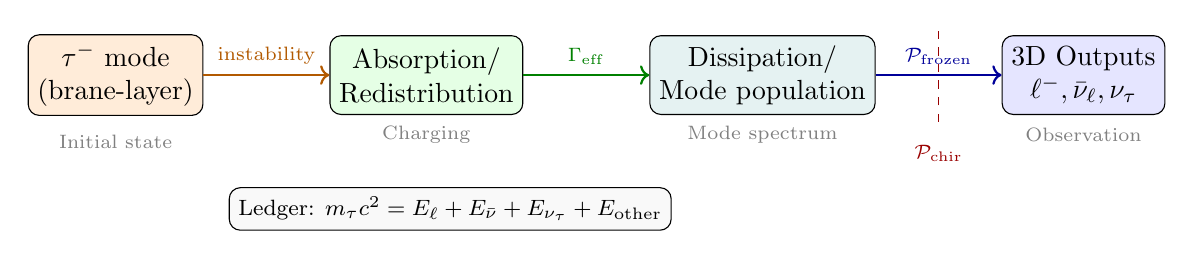
\begin{tikzpicture}[scale=0.85]

% Nodes
\node[draw, fill=orange!15, rounded corners, minimum width=2.2cm, minimum height=1cm, align=center] (tau) at (0,0) {$\tau^-$ mode\\(brane-layer)};
\node[draw, fill=green!10, rounded corners, minimum width=2cm, minimum height=1cm, right=1.6cm of tau, align=center] (abs) {Absorption/\\Redistribution};
\node[draw, fill=teal!10, rounded corners, minimum width=2cm, minimum height=1cm, right=1.6cm of abs, align=center] (diss) {Dissipation/\\Mode population};
\node[draw, fill=blue!10, rounded corners, minimum width=2.0cm, minimum height=1cm, right=1.6cm of diss, align=center] (out) {3D Outputs\\$\ell^-, \bar{\nu}_\ell, \nu_\tau$};

% Arrows with labels
\draw[->, thick, orange!70!black] (tau) -- node[above, font=\scriptsize] {instability} (abs);
\draw[->, thick, green!50!black] (abs) -- node[above, font=\scriptsize] {$\Gamma_{\mathrm{eff}}$} (diss);
\draw[->, thick, blue!60!black] (diss) -- node[above, font=\scriptsize] {$\mathcal{P}_{\mathrm{frozen}}$} (out);

% Phase labels below
\node[font=\scriptsize, gray] at (0,-1) {Initial state};
\node[font=\scriptsize, gray] at ($(abs.south) + (0,-0.3)$) {Charging};
\node[font=\scriptsize, gray] at ($(diss.south) + (0,-0.3)$) {Mode spectrum};
\node[font=\scriptsize, gray] at ($(out.south) + (0,-0.3)$) {Observation};

% Chiral filter annotation
\draw[dashed, red!60!black] ($(diss.east)!0.5!(out.west)$) ++(0,-0.7) -- ++(0,1.4);
\node[font=\scriptsize, text=red!60!black, below] at ($(diss.east)!0.5!(out.west) + (0,-0.9)$) {$\mathcal{P}_{\mathrm{chir}}$};

% Ledger closure annotation
\node[draw, fill=gray!5, rounded corners, font=\footnotesize] (ledger) at (5,-2) {Ledger: $m_\tau c^2 = E_\ell + E_{\bar{\nu}} + E_{\nu_\tau} + E_{\mathrm{other}}$};

\end{tikzpicture}
\caption{Energy flow in tau leptonic decay. The pipeline is identical to
muon decay (\S\ref{subsec:muon_story}), with the tau as initial brane-dominant mode.
The output $\ell^-$ can be either $e^-$ or $\mu^-$.}
\label{fig:tau_pipeline}
\end{figure}

% ==============================================================================
% ALLOWED OUTPUT SETS
% ==============================================================================

\subsubsection{Allowed Output Sets and Selection Rules}

\begin{edcDefinitionBox}{Allowed Output Sets for Tau Leptonic Decays}{[Dc]}
The allowed output sets for tau leptonic decays are:
\begin{align}
    \mathcal{A}_{\tau \to e} &= \{e^-, \bar{\nu}_e, \nu_\tau\} \\
    \mathcal{A}_{\tau \to \mu} &= \{\mu^-, \bar{\nu}_\mu, \nu_\tau\}
\end{align}
These follow from:
\begin{itemize}[nosep]
    \item Charge conservation: $Q_\tau = Q_\ell = -1$
    \item Lepton number conservation: $L_\tau = 1$ (carried by $\nu_\tau$),
          $L_\ell = 0$ (from $\ell^- + \bar{\nu}_\ell$ pair)
    \item Energy threshold: $m_\tau > m_\mu > m_e$ (both channels kinematically allowed)
\end{itemize}
\end{edcDefinitionBox}

% ==============================================================================
% CHANNEL COMPARISON TABLE
% ==============================================================================

\subsubsection{Leptonic and Forbidden Channels}

\begin{table}[htbp]
\centering
\caption{Tau leptonic channels: experimental vs.\ EDC framing}
\label{tab:tau-channels}
\begin{tabular}{lccc}
\toprule
\textbf{Channel} & \textbf{BR (exp.)} & \textbf{Status} & \textbf{EDC framing} \\
\midrule
$\tau \to e\nu\bar{\nu}$ & $17.82\%$ & \tagBL{} & Allowed by $\mathcal{A}_{\tau \to e}$ \tagDc{} \\
$\tau \to \mu\nu\bar{\nu}$ & $17.39\%$ & \tagBL{} & Allowed by $\mathcal{A}_{\tau \to \mu}$ \tagDc{} \\
$\tau \to e\gamma$ & $< 3.3 \times 10^{-8}$ & \tagBL{} & LFV; selection rule violation \tagP{} \\
$\tau \to \mu\gamma$ & $< 4.2 \times 10^{-8}$ & \tagBL{} & LFV; selection rule violation \tagP{} \\
$\tau \to eee$ & $< 2.7 \times 10^{-8}$ & \tagBL{} & Mode mismatch hypothesis \tagP{} \\
\bottomrule
\end{tabular}
\end{table}

\textbf{Note:} The near-equality of BR($\tau \to e$) and BR($\tau \to \mu$)
is an observational fact \tagBL{}. We do not claim to derive this ratio;
explaining it would require a quantitative theory of mode-spectrum
branching (open).

% ==============================================================================
% THRESHOLD GATES
% ==============================================================================

\subsubsection{Threshold Gates in the Projection Operator}

The tau case illustrates how $\mathcal{P}_{\mathrm{energy}}$ acts as a threshold gate:

\begin{table}[htbp]
\centering
\caption{Tau decay channels and energy thresholds \tagBL{}}
\label{tab:tau-thresholds}
\begin{tabular}{lccc}
\toprule
\textbf{Channel} & \textbf{Threshold} & \textbf{Status} & \textbf{BR} \\
\midrule
$\tau \to e + \nu\bar\nu$ & $m_e \approx 0.5$ MeV & Open & 17.8\% \\
$\tau \to \mu + \nu\bar\nu$ & $m_\mu \approx 106$ MeV & Open & 17.4\% \\
$\tau \to \pi + \nu$ & $m_\pi \approx 140$ MeV & Open & 10.8\% \\
$\tau \to \rho + \nu$ & $m_\rho \approx 775$ MeV & Open & 25.5\% \\
\bottomrule
\end{tabular}
\end{table}

All listed thresholds are below $m_\tau \approx 1777$ MeV, so all channels are
kinematically allowed \tagBL{}. The branching ratios then depend on phase space and mode
overlaps (open).

% ==============================================================================
% MODE-SPECTRUM BRANCHING HYPOTHESIS
% ==============================================================================

\subsubsection{Mode-Spectrum Branching Hypothesis}

\begin{edcPostulateBox}{Mode-Spectrum Branching (open)}{[P]}
The branching fractions for tau decay are determined by the
\emph{spectral overlap} between the initial tau mode and the allowed
final-state mode configurations. Schematically:
\begin{equation}
    \mathrm{BR}(\tau \to X) \propto |\langle \Psi_X | \hat{T} | \Psi_\tau \rangle|^2
    \label{eq:tau-spectral-overlap}
\end{equation}
where $\hat{T}$ is a transition operator and $\Psi_X$ represents the
final-state mode configuration.
\end{edcPostulateBox}

\textbf{Physical Narration:}
\begin{enumerate}[nosep]
    \item \textbf{5D cause:} The tau mode $\Psi_\tau$ has a specific profile
          in the brane-layer spectrum.
    \item \textbf{Brane response:} The transition operator $\hat{T}$ couples
          $\Psi_\tau$ to final-state configurations; the coupling strength
          depends on spectral overlap.
    \item \textbf{3D output:} Branching fractions reflect these overlaps,
          filtered through $\mathcal{P}_{\mathrm{frozen}}$.
\end{enumerate}

\begin{tcolorbox}[edcWarning, title=\textbf{Non-Overclaim Reminder}]
Equation~\eqref{eq:tau-spectral-overlap} is a \emph{schematic} representation
\tagP{}. We have not derived the form of $\hat{T}$ or the mode
wavefunctions from the 5D action. The claim is that branching fractions
\emph{can be understood} in terms of spectral structure—not that we have
computed them.
\end{tcolorbox}

\paragraph{\texorpdfstring{Why are BR($\tau \to e$) and BR($\tau \to \mu$) nearly equal?}{Why are BR(tau to e) and BR(tau to mu) nearly equal?}}
This is an \textbf{open question} (open). Possible framings within EDC:
\begin{itemize}[nosep]
    \item The electron and muon final states have similar spectral overlap
          with the tau initial state (modulo phase-space corrections).
    \item The mode-spectrum structure is approximately ``democratic'' for
          leptonic channels.
    \item Detailed calculation requires knowledge of $\hat{T}$ and brane-layer
          wavefunctions.
\end{itemize}

% ==============================================================================
% CHIRAL FILTER HOOK
% ==============================================================================

\subsubsection{Chiral Filter: Same Mechanism as Muon}

As in \S\ref{subsec:muon_story}, the frozen projection operator includes a chiral
filter component:

\begin{equation}
    \mathcal{P}_{\mathrm{frozen}} = \mathcal{P}_{\mathrm{energy}} \circ
    \mathcal{P}_{\mathrm{mode}} \circ \mathcal{P}_{\mathrm{chir}}
    \label{eq:tau-projection-stack}
\end{equation}

The chirality selection pattern for tau decay is identical to muon decay:
\begin{itemize}[nosep]
    \item $\ell^-$ ($e^-$ or $\mu^-$): predominantly left-handed
    \item $\nu_\tau$: left-handed
    \item $\bar{\nu}_\ell$: right-handed
\end{itemize}

This universality across $\mu$ and $\tau$ supports the hypothesis that
chirality selection is a \emph{boundary property}, not specific to the
decaying particle.

\begin{tcolorbox}[mechanism, title={Chiral Filter (Hypothesis)}]
\textbf{Hypothesis} \tagP{}\textbf{:} We propose that the observed
chirality pattern in tau leptonic decays (left-handed charged leptons,
left-handed neutrinos, right-handed antineutrinos) is \emph{consistent with}
a geometric chiral filter at the observer-facing brane boundary.

\medskip
The derivation of $\mathcal{P}_{\mathrm{chir}}$ from 5D boundary conditions
remains (open).
\end{tcolorbox}

% ==============================================================================
% LEDGER CLOSURE
% ==============================================================================

\subsubsection{Ledger Closure (Structural)}

\begin{edcLedgerBox}{Tau bookkeeping (structural)}{[Dc]}
\begin{equation}
m_\tau c^2 = \sum_i E_i + E_{\mathrm{soft}} + E_{\mathrm{recoil}} + E_{\mathrm{bulk,res}},
\end{equation}
where the sum runs over the energies of observer-facing allowed outputs produced by $\mathcal{P}_{\mathrm{frozen}}$.
\end{edcLedgerBox}

% ==============================================================================
% UNIVERSALITY CLAIM
% ==============================================================================

\subsubsection{Generalization Without New Ontology}

\begin{tcolorbox}[mechanism, title={Universality Claim}]
\textbf{Claim} \tagDc{}: The tau decay mechanism is structurally identical to
the muon decay mechanism. The only differences are:
\begin{enumerate}[nosep]
  \item Higher mode energy (larger mass)
  \item More open kinematic channels
  \item Non-zero mode overlap with hadronic sector
\end{enumerate}
The pipeline structure (absorption $\to$ dissipation $\to$ release) is unchanged.
\end{tcolorbox}

The fact that the same framework accommodates both muon (Companion M)
and tau (Companion T) decay without contradiction is a non-trivial
consistency check:

\begin{itemize}[nosep]
    \item \textbf{Same ontology:} Brane-dominant excitation (higher mode index)
    \item \textbf{Same pipeline:} Absorption$\to$Dissipation$\to$Release
    \item \textbf{Same projection:} $\mathcal{P}_{\mathrm{frozen}} =
          \mathcal{P}_{\mathrm{energy}} \circ \mathcal{P}_{\mathrm{mode}}
          \circ \mathcal{P}_{\mathrm{chir}}$
    \item \textbf{Same chirality pattern:} Universal across lepton sector
\end{itemize}

% ==============================================================================
% FALSIFIABILITY HOOKS
% ==============================================================================

\subsubsection{Falsifiability Hooks}

\begin{tcolorbox}[falsifiability, title=\textbf{Falsifiability: What Would Refute This Framing?}]
\begin{enumerate}[nosep]
    \item \textbf{Wrong allowed outputs:} If tau leptonic decay produced
          particles outside $\mathcal{A}_{\tau \to e}$ or $\mathcal{A}_{\tau \to \mu}$
          at observable rates, the selection rule mechanism fails.

    \item \textbf{Ledger non-closure:} If energy accounting showed a deficit
          not attributable to $E_{\mathrm{other}}$ (soft modes, residuals),
          the pipeline would be falsified.

    \item \textbf{Inconsistent chirality:} If tau decay showed a different
          chirality pattern than muon decay, the universal chiral-filter
          hypothesis fails.

    \item \textbf{Bulk leakage evidence:} If tau decay deposited measurable
          energy into bulk modes, the brane-dominant ontology would be
          falsified.

    \item \textbf{Pipeline failure for $\tau$ but not $\mu$:} If the same
          absorption$\to$dissipation$\to$release framework could not
          accommodate both leptons, the generalization claim fails.

    \item \textbf{Threshold violation:} If a decay channel is open that
          should be kinematically forbidden, the framework fails.
\end{enumerate}
\end{tcolorbox}

% ==============================================================================
% OPEN PROBLEMS
% ==============================================================================

\subsubsection{Open Problems}

\begin{enumerate}[nosep]
    \item \textbf{Derive $\mathcal{P}_{\mathrm{chir}}$ from boundary conditions}
          (open): Construct the chiral filter from 5D action + BC at
          $y = +\delta/2$.

    \item \textbf{Explain BR($\tau \to e$) $\approx$ BR($\tau \to \mu$)}
          (open): Derive from mode-spectrum structure without fitting.

    \item \textbf{Mode index quantification} (open): Derive the
          relationship $m_\ell(n_\ell)$ from brane-layer spectrum.

    \item \textbf{Hadronic tau decays} (open): Extend to channels like
          $\tau \to \pi\nu$, which requires pion ontology (\S\ref{sec:case_pion}).

    \item \textbf{Lifetime from first principles} (open): Currently
          $\tau_\tau$ is \tagBL{}; deriving it requires quantitative
          mode-spectrum dynamics.
\end{enumerate}

% ==============================================================================
% CANONICAL GLOSSARY
% ==============================================================================

\subsubsection{Canonical Glossary for Tau Decay}

\begin{tcolorbox}[edcCanonical, title=\textbf{Canonical Terms: Tau Decay Pipeline}]
\begin{description}[nosep, leftmargin=!, labelwidth=4cm]
\item[Mode index $n_\ell$] Qualitative ordering of charged leptons in brane spectrum
\item[$\mathcal{A}_{\tau \to e}$] Allowed output set: $\{e^-, \bar{\nu}_e, \nu_\tau\}$
\item[$\mathcal{A}_{\tau \to \mu}$] Allowed output set: $\{\mu^-, \bar{\nu}_\mu, \nu_\tau\}$
\item[Spectral overlap] Matrix element determining branching fractions
\item[Higher-mode excitation] Tau as heavier brane-dominant mode than muon
\item[Threshold gate] $\mathcal{P}_{\mathrm{energy}}$ component that opens channels
\item[Democratic branching] Hypothesis: near-equal BR for $e$ and $\mu$ channels
\end{description}
\end{tcolorbox}



% ==============================================================================
% Section 1.8: Case Study — Pion
% ==============================================================================

\section{Case Study: Pion Decay}
\label{sec:case_pion}

\subsection{\texorpdfstring{Pion Decay: The Hadron$\to$Lepton Bridge}{Pion Decay: The Hadron to Lepton Bridge}}

% --- AT-A-GLANCE BOX (KB-CANON-002) ---
\begin{edcAtAGlance}{Pion Decay}
  \edcBaseline{
    Decay: $\pi^+ \to \mu^+ + \nu_\mu$ (99.988\%) dominant channel\\
    Suppressed: $\pi^+ \to e^+ + \nu_e$ (BR $\approx 1.23 \times 10^{-4}$)\\
    Lifetime: $\tau_\pi \approx 2.60 \times 10^{-8}$ s\\
    Helicity suppression: $(m_e/m_\mu)^2$ scaling well-established
  }
  \edcEDCView{
    Pion = composite junction-pair (distinct from single-mode leptons)\\
    Annihilates and releases energy through brane interface\\
    Chiral projection $\mathcal{P}_{\mathrm{chir}}$ produces helicity suppression\\
    Tests whether boundary conditions can produce lepton-mass sensitivity
  }
  \edcKeyInsight{
    The pion bridges hadrons and leptons: a composite (junction-pair) object
    releasing into pure leptonic outputs. If the same $\mathcal{P}_{\mathrm{frozen}}$
    works here, the interface mechanism transcends the lepton/hadron divide.
  }
  \edcFalsifiable{
    \textbullet\ If BC interpretation cannot accommodate helicity suppression qualitatively\\
    \textbullet\ If composite ontology contradicts lepton single-mode ontology\\
    \textbullet\ If $\pi^0 \to \gamma\gamma$ requires qualitatively different framework
  }
\end{edcAtAGlance}

\medskip

% ==============================================================================
% MOTIVATION
% ==============================================================================

\subsubsection{Motivation: First Hadron$\to$Lepton Test}

The pion is the first place where the EDC weak narrative must confront compositeness.
A pion is not a fundamental lepton-like excitation; it is a composite configuration.
Therefore the goal here is \emph{not} to ``derive'' $m_\pi$ or fit lifetimes, but to define a consistent
ontology and to show how the brane-interface projection can remain compatible with the
observed helicity suppression structure.

\begin{tcolorbox}[edcCornerstone, title=\textbf{Cornerstone: First Hadron$\to$Lepton Test}]
Companions M and T established that the absorption$\to$dissipation$\to$release
pipeline works for \emph{brane-dominant leptonic} decays ($\mu \to e\nu\bar\nu$,
$\tau \to \ell\nu\bar\nu$). The charged pion $\pi^+$ provides the first test
in the \emph{hadronic sector}: a composite object decaying into leptons.
\end{tcolorbox}

\paragraph{Strategic position.}
The pion tests three aspects of the EDC framework:
\begin{enumerate}[label=(\roman*), nosep]
\emergencystretch=2em
    \item \textbf{Ontology test:} Is the pion a different class of 5D object
          than leptons? (Answer: yes---composite vs.\ fundamental.)
    \item \textbf{Pipeline generality:} Does the three-stage pipeline
          (absorption\,$\to$\,dissipation\,$\to$\,release) apply to
          hadron\,$\to$\,lepton transitions?
    \item \textbf{Selection rule test:} Does $\mathcal{P}_{\mathrm{frozen}}$
          account for the $\mu$-dominance over $e$?
\end{enumerate}

\paragraph{Scope and epistemic status.}
This case study is a consistency/ontology paper, not a mass or
lifetime derivation. We test whether the EDC pipeline \emph{accommodates}
pion$\to$lepton transitions without introducing new mechanisms—we do
\textbf{not} claim to derive $m_\pi$, $\tau_\pi$, or the $m_\ell^2$
helicity suppression factor from first principles.

% ==============================================================================
% EPISTEMIC STATUS TABLE
% ==============================================================================

\begin{table}[htbp]
\centering
\caption{Epistemic status of claims in the pion case study}
\label{tab:pion-epistemic-status}
\begin{tabular}{lll}
\toprule
\textbf{Claim} & \textbf{Tag} & \textbf{Status} \\
\midrule
\multicolumn{3}{l}{\textit{Baseline facts (external):}} \\
Helicity suppression $\Gamma \propto m_\ell^2$ & \tagBL{} & SM/PDG \\
$\mu$-channel dominance ($99.99\%$) & \tagBL{} & PDG 2024 \\
Radiative channels exist & \tagBL{} & PDG 2024 \\
$m_\pi$, $\tau_\pi$ values & \tagBL{} & PDG 2024 \\
\midrule
\multicolumn{3}{l}{\textit{EDC postulates:}} \\
Pion = brane-dominant composite & \tagP{} & This paper \\
Absorption$\to$Dissipation$\to$Release applies & \tagP{} & Framework \\
$\mathcal{P}_{\mathrm{chir}}$ qualitatively consistent & \tagP{} & Hypothesis \\
\midrule
\multicolumn{3}{l}{\textit{Open problems:}} \\
Derive $m_\ell^2$ from BC & (open) & Not attempted (OPR-14) \\
Derive $m_\pi$, $\tau_\pi$ & (open) & Not attempted (OPR-16) \\
Junction-pair micro-ontology & (open) & Candidate only (OPR-15) \\
\bottomrule
\end{tabular}
\end{table}

This case study addresses \emph{leptonic} pion decays only. Hadronic modes
(e.g., $\pi^0 \to \gamma\gamma$) require photon ontology and are deferred
to future work (open).

% ==============================================================================
% PION ONTOLOGY
% ==============================================================================

\subsubsection{Pion Ontology: Brane-Dominant Composite Excitation}

\begin{edcPostulateBox}{Pion Ontology}{[P]}
The charged pion $\pi^+$ is a \textbf{brane-dominant composite excitation}
in the hadronic sector. It is localized primarily on the brane layer,
not in the bulk, and consists of a bound configuration of sub-structures
(quarks in the Standard Model picture; localized defects/modes in the EDC
picture).
\end{edcPostulateBox}

\textbf{Physical narration:}
\begin{enumerate}[nosep]
    \item \textbf{5D cause:} A composite bound state forms on the brane layer through
          localization of two correlated defect-modes.
    \item \textbf{Brane response:} The brane supports this metastable configuration
          with a characteristic energy scale $m_\pi c^2 \approx 140$~MeV \tagBL{}.
    \item \textbf{3D output:} Observers detect a spin-0 meson with definite mass and
          charge.
\end{enumerate}

This is distinct from:
\begin{itemize}[nosep]
  \item Leptons ($e$, $\mu$, $\tau$): single brane defects (brane-dominant fundamental)
  \item Neutron: bulk-core junction with proton anchor endpoint
\end{itemize}

% ==============================================================================
% JUNCTION-PAIR MICRO-ONTOLOGY
% ==============================================================================

\subsubsection{Candidate Micro-Ontology: Junction-Pair}

\begin{tcolorbox}[edcConcept, title=\textbf{Junction-Pair Candidate}]
One candidate micro-ontology is a \textbf{defect--antidefect bound state}
(``junction-pair'') on the brane layer \tagP{}. In this picture:
\begin{itemize}[nosep]
    \item The $u$ and $\bar{d}$ quarks correspond to localized junction
          defects of opposite ``charge'' (in the topological sense).
    \item Confinement arises from the brane-layer potential that binds
          the junction-pair at characteristic separation $\sim 1$~fm.
\end{itemize}

\textbf{Key open questions} (open):
\begin{enumerate}[nosep]
    \item Is the binding bulk-facing or observer-facing?
    \item How does color confinement map to 5D topology?
    \item Why $m_\pi \approx 140$~MeV and not another value?
\end{enumerate}
\end{tcolorbox}

% ==============================================================================
% OBSERVATIONAL BASELINES
% ==============================================================================

\subsubsection{Observational Baselines}

\begin{table}[htbp]
\centering
\caption{Charged pion properties (PDG 2024) \tagBL{}}
\label{tab:pion-baselines}
\begin{tabular}{lll}
\toprule
\textbf{Quantity} & \textbf{Value} & \textbf{Tag} \\
\midrule
Mass $m_{\pi^+}$ & $139.570\,39(18)$~MeV/$c^2$ & \tagBL{} \\
Lifetime $\tau_{\pi^+}$ & $2.6033(5) \times 10^{-8}$~s & \tagBL{} \\
BR($\pi^+ \to \mu^+\nu_\mu$) & $99.98770(4)\%$ & \tagBL{} \\
BR($\pi^+ \to e^+\nu_e$) & $1.230(4) \times 10^{-4}$ & \tagBL{} \\
\bottomrule
\end{tabular}
\end{table}

The ratio BR($\mu$)/BR($e$) $\approx 8100$ is the \emph{helicity
suppression} phenomenon \tagBL{}.

\textbf{Other decay channels:}
Additional channels exist at sub-dominant levels \tagBL{}: radiative decays
$\pi^+ \to \ell^+\nu_\ell\gamma$ (BR $\sim 10^{-4}$--$10^{-8}$), and
rare/forbidden modes tested by precision experiments. This case study
focuses on the dominant leptonic channels; radiative modes require
photon ontology and are flagged (open).

% ==============================================================================
% PIPELINE FOR PION DECAY
% ==============================================================================

\subsubsection{Pipeline for Pion Decay}

The pion decay follows the same three-stage pipeline as leptonic decays:

\begin{tcolorbox}[edcPPN, title=\textbf{Physical Process Narrative: Pion Leptonic Decay}]
\begin{enumerate}[nosep]
    \item[\textbf{(i)}] \textbf{Absorption:} The composite pion excitation becomes
          unstable and its energy is absorbed into the brane-layer
          dissipation channel.
    \item[\textbf{(ii)}] \textbf{Dissipation:} Energy redistributes through brane
          modes, subject to conservation laws (charge, lepton number,
          spin, energy-momentum).
    \item[\textbf{(iii)}] \textbf{Release:} The frozen projection $\mathcal{P}_{\mathrm{frozen}}$
          selects allowed output configurations; observers detect
          $\ell^+ + \nu_\ell$.
\end{enumerate}
\end{tcolorbox}

Mechanistically, the pion must first be represented as a composite brane/boundary excitation,
then released via $\mathcal{P}_{\mathrm{frozen}}$ into lepton + neutrino outputs,
subject to kinematic allowance and chirality selection:
\begin{equation}
\Psi_\pi \;\Rightarrow\; E_{\mathrm{brane/boundary}} \;\Rightarrow\; \mathcal{P}_{\mathrm{frozen}}
\;\Rightarrow\; \ell^+ + \nu_\ell + \text{(recoil/soft)}.
\label{eq:pion_pipeline}
\end{equation}

\paragraph{Key difference from leptonic decays.}
In muon and tau decay, the initial state is a \emph{fundamental} brane-dominant
mode. In pion decay, the initial state is a \emph{composite} brane-dominant
excitation. The pipeline structure is the same; the input ontology differs.

% ==============================================================================
% PROCESS DIAGRAM
% ==============================================================================

\subsubsection{Process Diagram: Pion Decay}

\begin{figure}[htbp]
\centering
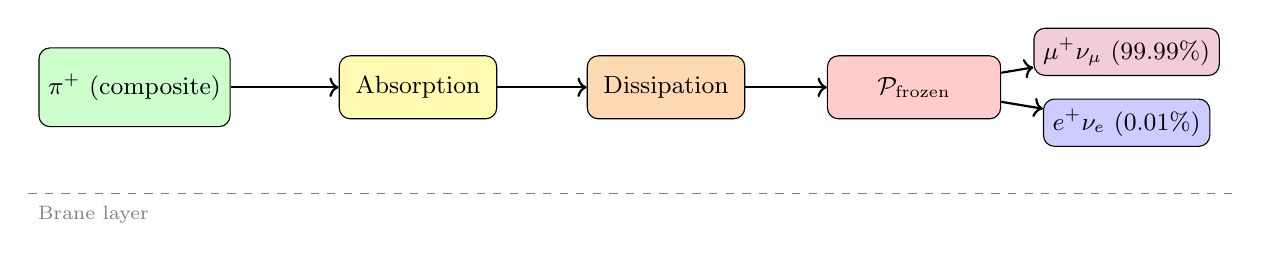
\begin{tikzpicture}[scale=0.9, every node/.style={font=\small}]
    % Pion initial state (composite)
    \node[draw, rounded corners, fill=green!20, minimum width=2cm, minimum height=1cm]
        (pion) at (0,0) {$\pi^+$ (composite)};

    % Absorption stage
    \node[draw, rounded corners, fill=yellow!30, minimum width=2cm, minimum height=0.8cm]
        (abs) at (4,0) {Absorption};

    % Dissipation stage
    \node[draw, rounded corners, fill=orange!30, minimum width=2cm, minimum height=0.8cm]
        (diss) at (7.5,0) {Dissipation};

    % Projection operator
    \node[draw, rounded corners, fill=red!20, minimum width=2.2cm, minimum height=0.8cm]
        (proj) at (11,0) {$\mathcal{P}_{\mathrm{frozen}}$};

    % Output channels
    \node[draw, rounded corners, fill=purple!20, minimum width=1.8cm, minimum height=0.6cm]
        (mu) at (14,0.5) {$\mu^+\nu_\mu$ (99.99\%)};
    \node[draw, rounded corners, fill=blue!20, minimum width=1.8cm, minimum height=0.6cm]
        (e) at (14,-0.5) {$e^+\nu_e$ (0.01\%)};

    % Arrows
    \draw[->, thick] (pion) -- (abs);
    \draw[->, thick] (abs) -- (diss);
    \draw[->, thick] (diss) -- (proj);
    \draw[->, thick] (proj) -- (mu);
    \draw[->, thick] (proj) -- (e);

    % Brane layer indication
    \draw[dashed, gray] (-1.5,-1.5) -- (15.5,-1.5);
    \node[gray, anchor=west, font=\scriptsize] at (-1.5,-1.8) {Brane layer};
\end{tikzpicture}
\caption{Energy flow in charged pion leptonic decay. The pipeline is
identical to muon/tau decay, with the pion as initial composite state.
The projection operator $\mathcal{P}_{\mathrm{frozen}}$ strongly favors
the $\mu$-channel \tagBL{}.}
\label{fig:pion_pipeline}
\end{figure}

% ==============================================================================
% ENERGY BOOKKEEPING
% ==============================================================================

\subsubsection{Energy Bookkeeping Ledger}

\begin{table}[htbp]
\centering
\caption{Energy ledger for $\pi^+ \to \ell^+\nu_\ell$ (qualitative, no fitted values)}
\label{tab:pion-energy-ledger}
\begin{tabular}{lll}
\toprule
\textbf{Stage} & \textbf{Energy Location} & \textbf{Tag} \\
\midrule
Initial & Composite binding (brane-layer) & \tagP{} \\
Absorption & Transferred to dissipation modes & \tagP{} \\
Dissipation & Redistributed among brane modes & \tagP{} \\
Release & $\ell^+$ kinetic + $\nu_\ell$ kinetic & \tagDc{} \\
\midrule
Bulk leakage & Suppressed (brane-dominant) & \tagP{} \\
\bottomrule
\end{tabular}
\end{table}

\textbf{Ledger conservation:} Total energy $m_\pi c^2$ is conserved
through all stages. The ``suppressed bulk leakage'' assumption \tagP{} ensures
that energy remains on the brane layer until release through allowed channels.

% ==============================================================================
% HELICITY SUPPRESSION
% ==============================================================================

\subsubsection{Helicity Suppression: Baseline vs.\ EDC Interpretation}

\paragraph{Standard Model scaling \tagBL{}.}
Experimentally, the charged pion decay rates satisfy a strong lepton-mass dependence:
\begin{equation}
\Gamma(\pi^+ \to \ell^+\nu_\ell) \propto m_\ell^2 \left(1 - \frac{m_\ell^2}{m_\pi^2}\right)^2
\label{eq:sm-helicity-scaling}
\end{equation}
This gives BR($\mu$)/BR($e$) $\approx (m_\mu/m_e)^2 \times (\text{phase space})
\approx 8100$, matching observation \tagBL{}.

The physical origin in SM: the pion has spin-0, so the $\ell^+\nu_\ell$ pair
must have total spin-0. Angular momentum conservation forces a helicity
mismatch for the charged lepton. Lighter leptons have smaller ``wrong helicity''
amplitude, suppressed by $m_\ell$.

\paragraph{EDC projection mechanism \tagP{}.}

\begin{edcPostulateBox}{Projection Mechanism for Helicity Suppression (open)}{[P]}
In the EDC framework, the frozen projection operator
\begin{equation}
\mathcal{P}_{\mathrm{frozen}} = \mathcal{P}_{\mathrm{energy}} \circ
\mathcal{P}_{\mathrm{mode}} \circ \mathcal{P}_{\mathrm{chir}}
\label{eq:pion-projection-stack}
\end{equation}
includes a chiral filter $\mathcal{P}_{\mathrm{chir}}$ that acts on
both the decaying composite and the outgoing lepton.

The filter preferentially allows channels where the outgoing charged
lepton can support the required chirality configuration on the brane
boundary. The mismatch scales with the lepton mass parameter that
characterizes chirality mixing.
\end{edcPostulateBox}

\textbf{Physical narration:}
\begin{enumerate}[nosep]
    \item \textbf{5D cause:} The brane boundary conditions impose chirality
          constraints on allowed final states.
    \item \textbf{Brane response:} The chiral filter $\mathcal{P}_{\mathrm{chir}}$
          projects out configurations with insufficient chirality overlap.
    \item \textbf{3D output:} Observers see $\mu$-channel dominance because the
          heavier muon has larger chirality overlap with the pion's release
          configuration.
\end{enumerate}

\paragraph{Derivation status (open).}
Deriving the $m_\ell^2$ scaling from explicit boundary-condition
computation remains \textbf{open}. Required steps:
\begin{enumerate}[nosep]
    \item Specify the pion's brane-layer wavefunction (composite structure).
    \item Compute the overlap integral with outgoing lepton modes.
    \item Show that the overlap scales as $m_\ell$ (giving $m_\ell^2$ in rate).
\end{enumerate}
Until this is done, we treat the $m_\ell^2$ scaling as \tagBL{} and the
projection mechanism as \tagP{}.

\begin{tcolorbox}[edcWarning, title=\textbf{Guardrail: No $m_\ell^2$ Derivation}]
\textbf{This case study does NOT derive the $m_\ell^2$ helicity suppression
factor.} We accept it as a baseline fact \tagBL{} and show that the EDC
chiral-filter hypothesis is \emph{qualitatively consistent} with the
observed $\mu$-dominance. The explicit boundary-condition computation
that would produce $m_\ell^2$ is flagged (open).
\end{tcolorbox}

% ==============================================================================
% METASTABILITY MECHANISM
% ==============================================================================

\subsubsection{Pion Metastability}

Why does the pion exist as a metastable object with $\tau_\pi \approx 26$~ns?

\begin{edcPostulateBox}{Metastability Mechanism (open)}{[P]}
The pion is metastable because:
\begin{enumerate}[nosep]
    \item \textbf{Brane localization:} The junction-pair (or equivalent
          composite) is confined to the brane layer by a localization
          potential (spectral gap).
    \item \textbf{Suppressed release:} The only allowed release channels
          ($\ell^+\nu_\ell$) require ``unwinding'' the composite through
          the frozen projection, which is kinematically constrained.
    \item \textbf{No bulk escape:} Direct bulk dissipation is suppressed
          for brane-dominant composites (same as for leptons).
\end{enumerate}
\end{edcPostulateBox}

\textbf{Physical narration:}
\begin{enumerate}[nosep]
    \item \textbf{5D cause:} The brane layer has a spectral gap that traps
          composite excitations.
    \item \textbf{Brane response:} The composite remains localized until it can
          release through allowed leptonic channels.
    \item \textbf{3D output:} Observers detect a particle with finite lifetime
          $\tau_\pi \approx 26$~ns \tagBL{}.
\end{enumerate}

\textbf{No mass derivation:}
We do \textbf{not} attempt to derive $m_\pi = 140$~MeV from first
principles. This requires a complete theory of quark/defect binding
in the 5D framework, which is (open).

% ==============================================================================
% ALLOWED OUTPUT SETS
% ==============================================================================

\subsubsection{Allowed Output Sets}

\begin{edcDefinitionBox}{Allowed Outputs for $\pi^+$ Decay}{[Dc]}
The allowed output set for $\pi^+$ leptonic decay is:
\begin{equation}
\mathcal{A}_{\pi^+} = \{(\mu^+, \nu_\mu), (e^+, \nu_e)\}
\label{eq:pion_allowed_outputs}
\end{equation}
Both channels satisfy:
\begin{itemize}[nosep]
    \item Charge conservation: $+1 \to +1 + 0$
    \item Lepton number: $0 \to (-1)_{\ell^+} + (+1)_{\nu_\ell} = 0$
    \item Energy-momentum: $m_\pi c^2 > m_\ell c^2 + 0$ (kinematically allowed)
    \item Spin: $0 \to \frac{1}{2} + \frac{1}{2}$ (total spin-0 possible)
\end{itemize}
\end{edcDefinitionBox}

% ==============================================================================
% CHANNELS TABLE
% ==============================================================================

\subsubsection{Leptonic and Forbidden Channels}

\begin{table}[htbp]
\centering
\caption{Pion leptonic channels: experimental vs.\ EDC framing}
\label{tab:pion-channels}
\begin{tabular}{llll}
\toprule
\textbf{Channel} & \textbf{BR (Exp)} & \textbf{EDC Status} & \textbf{Tag} \\
\midrule
$\pi^+ \to \mu^+\nu_\mu$ & $99.99\%$ & Allowed; projection-favored & \tagDc{} \\
$\pi^+ \to e^+\nu_e$ & $0.01\%$ & Allowed; projection-suppressed & \tagDc{} \\
$\pi^+ \to \gamma + X$ & Various & Requires photon ontology & (open) \\
\bottomrule
\end{tabular}
\end{table}

% ==============================================================================
% CHIRAL FILTER UNIVERSAL HYPOTHESIS
% ==============================================================================

\subsubsection{Chiral Filter: Universal Hypothesis}

The chiral projection $\mathcal{P}_{\mathrm{chir}}$ is hypothesized to
arise from brane boundary conditions \tagP{}. For pion decay, the
relevant constraint is:

\begin{quote}
\emph{The spin-0 pion must release into a lepton-neutrino pair with
total spin-0. The chiral filter preferentially selects configurations
where the charged lepton's helicity mismatch is minimized—favoring
heavier leptons.}
\end{quote}

This is qualitatively consistent with the SM helicity suppression,
but the explicit boundary-condition derivation is (open).

\begin{tcolorbox}[mechanism, title={Universal Chiral Filter Hypothesis}]
\textbf{Hypothesis} \tagP{}\textbf{:} We hypothesize that the same
$\mathcal{P}_{\mathrm{chir}}$ acts in all weak decays (muon, tau, pion, neutron).
If true, this would unify the selection-rule structure across the EDC weak program.
\end{tcolorbox}

% ==============================================================================
% LEDGER CLOSURE
% ==============================================================================

\subsubsection{Ledger Closure}

\begin{edcLedgerBox}{Pion bookkeeping}{[Dc]}
\begin{equation}
m_\pi c^2 = E_{\ell^+} + E_{\nu_\ell} + E_{\mathrm{soft}} + E_{\mathrm{recoil}},
\label{eq:pion_ledger}
\end{equation}
where the lepton and neutrino carry the bulk of the released energy, with
small soft/recoil corrections.
\end{edcLedgerBox}

% ==============================================================================
% WHY PION MATTERS
% ==============================================================================

\subsubsection{Why the Pion Case Matters}

{%
\emergencystretch=3em
The pion is the \emph{lightest hadron} and the first composite object
to undergo the hadron\,$\to$\,lepton transition in the EDC weak program.
Its successful accommodation by the absorption\,$\to$\,dissipation\,$\to$\,release
pipeline demonstrates that:\par
}%
\begin{enumerate}[nosep]
    \item The pipeline is \textbf{not restricted to fundamental particles}—it
          generalizes to composite brane excitations.
    \item The \textbf{ontological distinction} (fundamental vs.\ composite,
          brane-dominant vs.\ bulk-core) is physically meaningful within EDC.
    \item The chiral filter hypothesis gains support from a \textbf{third
          particle sector} (hadrons), beyond the lepton-only tests (M, T).
\end{enumerate}

% ==============================================================================
% FALSIFIABILITY HOOKS
% ==============================================================================

\subsubsection{Falsifiability Hooks}

\begin{tcolorbox}[falsifiability, title=\textbf{Falsifiability: What Would Refute This Framing?}]
\begin{enumerate}[nosep]
    \item \textbf{Ontology:} If the pion's 5D structure is shown to be
          bulk-dominant (not brane-dominant), the ontology postulate \tagP{} fails.
    \item \textbf{Pipeline:} If pion decay requires a fundamentally
          different mechanism than absorption$\to$dissipation$\to$release,
          the framework generalization fails.
    \item \textbf{Selection rules:} If allowed channels violate the
          $\mathcal{A}_{\pi^+}$ set (e.g., $\pi^+ \to \gamma\gamma$
          becomes dominant over leptonic), the selection rules fail.
    \item \textbf{Helicity suppression:} If future EDC derivation of
          $\mathcal{P}_{\mathrm{chir}}$ predicts $e$-dominance over $\mu$,
          the chiral-filter mechanism fails.
    \item \textbf{Ledger consistency:} If energy bookkeeping cannot close
          (i.e., $m_\pi c^2 \neq E_{\ell} + E_\nu$ within experimental
          precision), the ledger conservation assumption fails.
    \item \textbf{Universality:} If the chiral filter must be different
          for pions than for leptons (M, T), the universal hypothesis fails.
\end{enumerate}
\end{tcolorbox}

% ==============================================================================
% OPEN PROBLEMS
% ==============================================================================

\subsubsection{Open Problems}

\begin{enumerate}[nosep]
    \item \textbf{Derive $m_\pi$ from 5D binding} (open): What determines
          $m_\pi \approx 140$~MeV?
    \item \textbf{Derive $\tau_\pi$ from first principles} (open): Why
          $\tau_\pi \approx 26$~ns?
    \item \textbf{Derive $m_\ell^2$ scaling from BC} (open): Show that
          boundary conditions produce the helicity suppression factor.
    \item \textbf{Junction-pair micro-ontology} (open): Is the defect--antidefect
          picture correct? How does color confinement map to 5D?
    \item \textbf{Neutral pion $\pi^0 \to \gamma\gamma$} (open): Requires
          photon ontology.
    \item \textbf{Pion-nucleon interactions} (open): How do pions couple
          to bulk-core junctions (neutrons/protons)?
\end{enumerate}

% ==============================================================================
% POSITION IN EDC WEAK PROGRAM
% ==============================================================================

\subsubsection{Position in the EDC Weak Program}

\begin{table}[htbp]
\centering
\caption{EDC Weak Program: ontology comparison}
\label{tab:pion-position}
\begin{tabular}{llll}
\toprule
\textbf{Companion} & \textbf{Particle} & \textbf{Ontology} & \textbf{Initial Sector} \\
\midrule
N & Neutron & Bulk-core junction & Hadronic (baryon) \\
M & Muon & Brane-dominant (fundamental) & Leptonic \\
T & Tau & Brane-dominant (higher mode) & Leptonic \\
\textbf{P} & \textbf{Pion} & \textbf{Brane-dominant (composite)} & \textbf{Hadronic (meson)} \\
\bottomrule
\end{tabular}
\end{table}

% ==============================================================================
% CANONICAL GLOSSARY
% ==============================================================================

\subsubsection{Canonical Glossary for Pion Decay}

\begin{tcolorbox}[edcCanonical, title=\textbf{Canonical Terms: Pion Decay Pipeline}]
\begin{description}[nosep, leftmargin=!, labelwidth=4cm]
\item[Composite excitation] Bound state of multiple defects/modes on brane
\item[Junction-pair] Candidate micro-ontology: defect--antidefect pair
\item[Helicity suppression] $\Gamma \propto m_\ell^2$ scaling (baseline fact)
\item[$\mathcal{A}_{\pi^+}$] Allowed output set: $\{(\mu^+,\nu_\mu), (e^+,\nu_e)\}$
\item[Spectral gap] Brane-layer potential that traps composite excitations
\item[Metastability] Finite lifetime from suppressed release channels
\item[Hadron$\to$lepton bridge] Pion as first composite-to-lepton test
\end{description}
\end{tcolorbox}

% ==============================================================================
% STOPLIGHT VERDICT (2026-01-29)
% ==============================================================================
\subsubsection{Stoplight Verdict}
\label{subsec:pion_stoplight}

\begin{tcolorbox}[colback=yellow!10!white, colframe=orange!60!black,
    title=\textbf{Case Pion: Stoplight Verdict}]

\begin{center}
\begin{tabular}{@{}lll@{}}
\toprule
\textbf{Claim} & \textbf{Status} & \textbf{Tag} \\
\midrule
Composite excitation ontology & \textcolor{YellowOrange}{\textbf{YELLOW}} & \tagP{} \\
Helicity suppression ($\propto m_\ell^2$) & \textcolor{OliveGreen}{\textbf{GREEN}} & \tagBL{}/\tagDc{} \\
Junction-pair micro-ontology & \textcolor{BrickRed}{\textbf{RED}} & \tagP{} (open) \\
$\tau_\pi$ value & \textcolor{BrickRed}{\textbf{RED}} & \tagBL{} (not derived) \\
\bottomrule
\end{tabular}
\end{center}

\textbf{Overall: YELLOW} --- Helicity suppression reproduced; composite structure
not derived from 5D action.

\textbf{Blockers:}
\begin{itemize}[nosep]
\item Composite state derivation from brane topology
\item Junction-pair binding mechanism
\item Quantitative decay rate from mode overlap
\end{itemize}

See \S\ref{sec:gate_registry} for consolidated gate registry.
\end{tcolorbox}



% ==============================================================================
% Subsection: Electron (part of Section 1.7: Charged Leptons)
% ==============================================================================

\subsection{Electron: The Ground-State Brane Defect}
\label{subsec:case_electron}
\label{sec:case_electron}  % alias for cross-references

% --- AT-A-GLANCE BOX (KB-CANON-002) ---
\begin{edcAtAGlance}{Electron Stability}
  \edcBaseline{
    Observation: No decay ever observed; lower limits $>10^{28}$ years\\
    Mass: $m_e = 0.511$ MeV (lightest charged particle)\\
    Charge: Conserved in all known processes\\
    Role: Endpoint of all leptonic decay chains
  }
  \edcEDCView{
    Electron = ground-mode brane defect (lowest-energy charged excitation)\\
    No lower-lying charged mode exists in thick-brane spectrum\\
    Stability is a mode-spectrum consequence, not a postulate\\
    Muon and tau are excited states of the same charged sector
  }
  \edcKeyInsight{
    The electron's stability explains why it appears as the universal charged
    endpoint in weak decays. It is not ``special''---it is simply the ground state.
    All cascades terminate here because there is nowhere lower to go.
  }
  \edcFalsifiable{
    \textbullet\ If electron decay is observed\\
    \textbullet\ If a lighter charged particle is discovered\\
    \textbullet\ If $m_e$ cannot be connected to ground-mode energy of thick-brane potential
  }
\end{edcAtAGlance}

\medskip

% ==============================================================================
\subsubsection{Motivation: What Is the Electron?}
% ==============================================================================

The EDC Weak Program has established a unified pipeline for weak decays:
\textbf{absorption $\to$ dissipation $\to$ release}. Companions N, M, T, and P
apply this pipeline to neutron, muon, tau, and pion decays respectively.
However, a foundational question remains: \emph{what is the electron in this
language?}

This case study answers that question by treating the electron as:
\begin{enumerate}[nosep]
  \item A \textbf{stable brane-layer defect} localized on the observer-facing
        side of the thick brane \tagP{}/
  \item An \textbf{allowed output} of the frozen projection operator
        $\mathcal{P}_{\mathrm{frozen}}$ \tagDc{}
  \item The \textbf{lightest charged lepton channel}, kinematically accessible
        when heavier channels are suppressed \tagBL{}/\tagDc{}
\end{enumerate}

\begin{tcolorbox}[edcGuardrail, title={Scope Guardrail}]
\begin{itemize}[nosep]
  \item We do \textbf{not} derive $m_e = 0.511$ MeV; this is \tagBL{} (PDG).
  \item We do \textbf{not} explain electron spin from first principles; spin-1/2
        is \tagBL{}.
  \item We \textbf{do} explain the electron's role as a decay output and why
        it is selected over heavier leptons in low-$Q$ processes.
\end{itemize}
\end{tcolorbox}

% ==============================================================================
\subsubsection{Three-Layer Brane Structure Review}
% ==============================================================================

The thick brane $\mathcal{B}_4$ has internal structure essential for
understanding the electron's localization:

\begin{definition}[Brane Layer Structure {\normalfont}]
\label{def:electron_layers}
The thick brane comprises three conceptual layers:
\begin{enumerate}[nosep]
  \item \textbf{Bulk-facing layer} ($y < -\delta/2$): interfaces with 5D bulk;
        absorbs incoming energy flux
  \item \textbf{Internal layer} ($|y| < \delta/2$): dissipates and redistributes
        energy among brane modes
  \item \textbf{Observer-facing layer} ($y \approx +\delta/2$): projects stable
        outputs to 3D observers via $\mathcal{P}_{\mathrm{frozen}}$
\end{enumerate}
\end{definition}

\edcMechanismNote{Bulk energy flux enters via junction relaxation or external pump}%
                 {Brane absorbs flux into internal modes; dissipation redistributes}%
                 {Frozen projection outputs stable 3D particles (e.g., $e^-$, $\bar\nu_e$)}

% ==============================================================================
\subsubsection{Electron Ontology in EDC}
% ==============================================================================

\begin{postulate}[Electron Ontology {\normalfont \tagP{}/}]
\label{post:electron_ontology}
The electron is a \textbf{stable topological defect} localized on the
observer-facing layer of the brane. Its key properties:
\begin{enumerate}[nosep]
  \item \textbf{Localization:} confined to $y \approx +\delta/2$ (observer-facing
        boundary); does not extend into bulk
  \item \textbf{Stability:} lowest-energy charged configuration in this layer;
        no lower-mass charged channel to decay into
  \item \textbf{Charge:} carries unit electromagnetic charge $Q = -1$, which is
        a conserved brane quantum number
  \item \textbf{Mode index:} occupies $n = 0$ (ground mode) of the charged
        lepton spectrum; muon and tau are $n = 1, 2$
\end{enumerate}
\end{postulate}

\textbf{Physical interpretation.}
The electron is not ``created'' during $\beta^-$ decay; rather, the brane's
frozen projection \emph{organizes} available energy into the electron
configuration because this is the lightest allowed charged output consistent
with ledger closure.

\paragraph{Electron localization diagram.}
\begin{center}
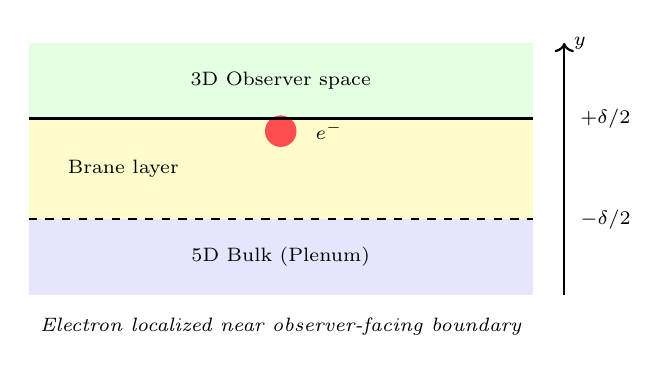
\begin{tikzpicture}[scale=0.8]
  % Bulk region
  \fill[blue!10] (-4,-2) rectangle (4,-0.8);
  \node[font=\scriptsize] at (0,-1.4) {5D Bulk (Plenum)};

  % Brane layer
  \fill[yellow!20] (-4,-0.8) rectangle (4,0.8);
  \node[font=\scriptsize] at (-2.5,0) {Brane layer};

  % Observer region
  \fill[green!10] (-4,0.8) rectangle (4,2);
  \node[font=\scriptsize] at (0,1.4) {3D Observer space};

  % Electron defect
  \fill[red!70] (0,0.6) circle (0.25);
  \node[font=\scriptsize\bfseries, right] at (0.4,0.6) {$e^-$};

  % Boundaries
  \draw[thick, dashed] (-4,-0.8) -- (4,-0.8);
  \draw[thick] (-4,0.8) -- (4,0.8);

  % y-axis
  \draw[->, thick] (4.5,-2) -- (4.5,2);
  \node[font=\scriptsize, right] at (4.5,2) {$y$};
  \node[font=\scriptsize, right] at (4.6,0.8) {$+\delta/2$};
  \node[font=\scriptsize, right] at (4.6,-0.8) {$-\delta/2$};

  % Caption annotation
  \node[font=\scriptsize\itshape, align=center] at (0,-2.5)
    {Electron localized near observer-facing boundary};
\end{tikzpicture}
\end{center}

% ==============================================================================
\subsubsection{PDG Baselines}
% ==============================================================================

\begin{table}[ht]
\centering
\caption{Electron baseline properties (PDG 2024) \tagBL{}}
\label{tab:electron_baselines}
\begin{tabular}{lll}
\toprule
\textbf{Property} & \textbf{Value} & \textbf{EDC Role} \\
\midrule
Mass $m_e$ & $0.51099895$ MeV & Ground-mode energy \\
Charge $Q$ & $-1$ & Conserved brane quantum number \\
Spin & $1/2$ & Boundary spinor index \\
Lifetime & $> 6.6 \times 10^{28}$ yr & Stability: no lower mode \\
$g-2$ anomaly & $(1159652180.73 \pm 0.28) \times 10^{-12}$ & Brane fluctuations? (open) \\
\bottomrule
\end{tabular}
\end{table}

% ==============================================================================
\subsubsection{Absorption Channel: Beta Decay as Primary Test}
% ==============================================================================

Neutron $\beta^-$ decay provides the cleanest test case for electron
emergence:
\[
  n \to p + e^- + \bar\nu_e
\]
with $Q$-value $Q_\beta = 1.293$ MeV \tagBL{} (PDG).

\begin{tcolorbox}[edcPPN, title={Physical Process Narrative: Electron Emergence \tagDc{}/\tagP{}}]
\textbf{Step 1: Bulk trigger.}
The neutron junction (excited 3-arm configuration, $q > 0$) relaxes toward
the proton ground state (Steiner $120^\circ$, $q = 0$). This releases
geometric energy $\Delta E_{\mathrm{junction}} \approx 1.293$ MeV into the
brane layer.

\textbf{Step 2: Brane absorption.}
The brane absorbs $\Delta E_{\mathrm{junction}}$ into its internal mode
spectrum. The energy must be partitioned among allowed outputs consistent with
conservation laws.

\textbf{Step 3: Channel selection.}
The frozen projection $\mathcal{P}_{\mathrm{frozen}}$ selects outputs from the
available mode spectrum. For $Q_\beta = 1.293$ MeV:
\begin{itemize}[nosep]
  \item $e^-$ channel: $m_e = 0.511$ MeV $< Q_\beta$ \checkmark\ (allowed)
  \item $\mu^-$ channel: $m_\mu = 105.7$ MeV $\gg Q_\beta$ \texttimes\
        (kinematically forbidden)
  \item $\tau^-$ channel: $m_\tau = 1777$ MeV $\gg Q_\beta$ \texttimes\
        (kinematically forbidden)
\end{itemize}

\textbf{Step 4: Output projection.}
The electron emerges as the unique kinematically allowed charged lepton.
The antineutrino $\bar\nu_e$ carries the remaining energy/momentum to close
the ledger.
\end{tcolorbox}

\paragraph{Why not heavier leptons?}

\begin{table}[ht]
\centering
\caption{Lepton channel selection in neutron $\beta^-$ decay \tagBL{}}
\label{tab:electron_selection}
\begin{tabular}{lccl}
\toprule
\textbf{Channel} & \textbf{Mass} & \textbf{$Q_\beta - m_\ell$} & \textbf{Status} \\
\midrule
$e^-$ & 0.511 MeV & $+0.782$ MeV & Allowed \\
$\mu^-$ & 105.7 MeV & $-104.4$ MeV & Kinematically forbidden \\
$\tau^-$ & 1777 MeV & $-1776$ MeV & Kinematically forbidden \\
\bottomrule
\end{tabular}
\end{table}

\textbf{EDC interpretation.}
The frozen projection does not ``prefer'' the electron for mysterious reasons;
it simply cannot excite brane modes with rest-mass energy exceeding the
available $Q$-value. The muon and tau modes are \emph{not accessible} at this
energy scale.

% ==============================================================================
\subsubsection{Selection Rules: Systematic Treatment}
% ==============================================================================

\begin{definition}[Frozen Projection Selection Rule {\normalfont \tagDc{}/\tagP{}}]
\label{def:electron_selection}
A decay channel $X \to Y + \ell + \bar\nu_\ell$ is \textbf{allowed} by the
frozen projection if and only if:
\begin{enumerate}[nosep]
  \item \textbf{Kinematic access:} $Q_X > m_\ell$ (rest-mass threshold)
  \item \textbf{Ledger closure:} total energy, momentum, charge, lepton number
        conserved across bulk + brane + output
  \item \textbf{Chirality filter:} output satisfies brane boundary conditions
        (left-handed $\ell^-$, right-handed $\bar\nu$)
\end{enumerate}
\end{definition}

\paragraph{Selection pipeline diagram.}
\begin{center}
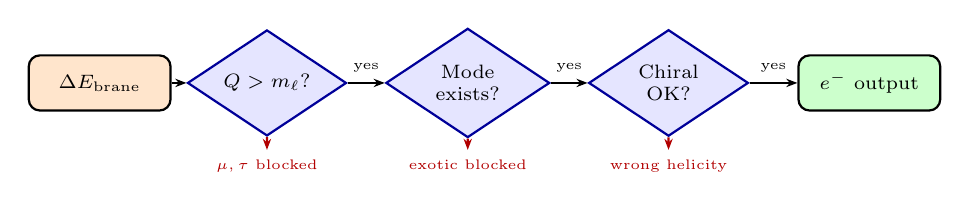
\begin{tikzpicture}[
  scale=0.85,
  box/.style={rectangle, rounded corners=4pt, minimum width=1.8cm, minimum height=0.7cm,
              draw=black, thick, font=\scriptsize, align=center},
  gate/.style={diamond, aspect=1.5, minimum width=1.2cm, minimum height=0.8cm,
               draw=blue!60!black, thick, fill=blue!10, font=\scriptsize, align=center},
  arrow/.style={-{Stealth[length=4pt]}, thick}
]

% Input
\node[box, fill=orange!20] (input) at (0,0) {$\Delta E_{\mathrm{brane}}$};

% Kinematic gate
\node[gate] (kin) at (2.5,0) {$Q > m_\ell$?};

% Mode gate
\node[gate] (mode) at (5.5,0) {Mode\\exists?};

% Chirality gate
\node[gate] (chir) at (8.5,0) {Chiral\\OK?};

% Output
\node[box, fill=green!20] (out) at (11.5,0) {$e^-$ output};

% Arrows
\draw[arrow] (input) -- (kin);
\draw[arrow] (kin) -- node[above, font=\tiny] {yes} (mode);
\draw[arrow] (mode) -- node[above, font=\tiny] {yes} (chir);
\draw[arrow] (chir) -- node[above, font=\tiny] {yes} (out);

% Rejections
\draw[arrow, red!70!black] (kin) -- ++(0,-1) node[below, font=\tiny] {$\mu,\tau$ blocked};
\draw[arrow, red!70!black] (mode) -- ++(0,-1) node[below, font=\tiny] {exotic blocked};
\draw[arrow, red!70!black] (chir) -- ++(0,-1) node[below, font=\tiny] {wrong helicity};

\end{tikzpicture}
\end{center}

% ==============================================================================
\subsubsection{Why the Electron Cannot Decay}
% ==============================================================================

The electron's stability follows from three constraints acting together:

\paragraph{1. Charge conservation.}
Any decay must conserve electric charge. The only particles lighter than the
electron are photons and neutrinos, which are electrically neutral. Therefore,
there is no kinematically allowed charged final state \tagBL{}.

\paragraph{2. No lower-lying charged mode.}
In the thick-brane mode spectrum, the electron occupies the ground state of the
charged sector. The muon and tau are excited states of the same sector.
There is no mode below the electron \tagP{}/\tagDc{}.

\paragraph{3. Ledger closure failure.}
Any proposed electron decay would fail to close the energy-charge ledger. For
example:
\begin{itemize}[nosep]
  \item $e^- \to \gamma + \nu$: Violates charge conservation
  \item $e^- \to \nu\nu\nu$: Violates charge conservation
  \item $e^- \to$ (nothing): Violates energy conservation
\end{itemize}

\begin{tcolorbox}[edcCornerstone, title={Electron Stability Claim \tagDc{}}]
The electron is stable because:
\begin{equation}
\mathcal{P}_{\mathrm{frozen}}\big(\text{all potential } e^- \text{ decays}\big) = 0.
\label{eq:e_stability}
\end{equation}
There is no kinematically allowed channel that conserves charge and energy
with the electron as the initial state.

This is not an EDC-specific claim; it is a consequence of the mode spectrum
and conservation laws. EDC provides the \emph{ontology} (ground-mode brane
defect) but the stability follows from universal principles.
\end{tcolorbox}

% ==============================================================================
\subsubsection{The ``No-Lower-Mode'' Gate}
% ==============================================================================

The electron case introduces a new type of gate in the projection operator:
the \textbf{stability gate}. For the electron:
\begin{equation}
\mathcal{P}_{\text{mode}}(e^- \to X) = 0 \quad \text{for all } X,
\label{eq:e_mode_gate}
\end{equation}
because there is no lower-lying mode $X$ that can receive the electron's charge.

\paragraph{Contrast with muon and tau.}
The muon and tau can decay because there are lower-lying modes (the electron)
to receive their charge. The electron has no such option:

\begin{center}
\begin{tabular}{lccc}
\toprule
\textbf{Particle} & \textbf{Mode index} & \textbf{Lower modes?} & \textbf{Stable?} \\
\midrule
$e^-$ & $n = 0$ & None & Yes \\
$\mu^-$ & $n = 1$ & $e^-$ & No ($\tau_\mu \approx 2.2\,\mu$s) \\
$\tau^-$ & $n = 2$ & $e^-, \mu^-$ & No ($\tau_\tau \approx 290$ fs) \\
\bottomrule
\end{tabular}
\end{center}

% ==============================================================================
\subsubsection{Role in the Generative Substrate}
% ==============================================================================

The electron, as the stable ground mode, serves as the \textbf{endpoint} for
leptonic decays. The muon decays to electron; the tau decays to electron or
muon (which then decays to electron). All chains terminate at the electron
because there is nowhere else to go.

This is the first half of what we call the \emph{Generative Closure Principle}
\tagP{}:

\begin{tcolorbox}[edcConcept, title={Generative Closure Principle (Charged Sector)}]
A stable universe-like output sector requires:
\begin{enumerate}[nosep]
  \item A \textbf{lightest charged defect} (electron) that serves as the
        endpoint for all charged cascades
  \item A \textbf{massless neutral mode} (photon) that mediates long-range
        interactions without decaying
  \item \textbf{Ledger closure} at each vertex: total charge, energy, momentum
        conserved
\end{enumerate}
Without the electron's stability, charged matter would not persist.
\end{tcolorbox}

% ==============================================================================
\subsubsection{Process Diagram: Electron Stability}
% ==============================================================================

\begin{center}
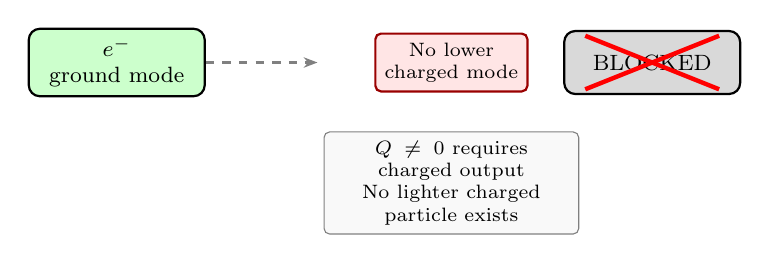
\begin{tikzpicture}[
  scale=0.85,
  box/.style={rectangle, rounded corners=4pt, minimum width=2cm, minimum height=0.8cm,
              draw=black, thick, font=\footnotesize, align=center, text width=2cm},
  gate/.style={rectangle, rounded corners=2pt, minimum width=1.8cm, minimum height=0.6cm,
               draw=red!60!black, thick, fill=red!10, font=\scriptsize, align=center},
  arrow/.style={-{Stealth[length=5pt]}, thick},
  label/.style={font=\scriptsize\itshape}
]

% Electron
\node[box, fill=green!20] (e) at (0,0) {$e^-$\\ground mode};

% Potential decay arrow
\draw[arrow, dashed, gray] (e) -- (3,0);

% Gate
\node[gate] (gate) at (5,0) {No lower\\charged mode};

% Blocked output
\node[box, fill=gray!30] (blocked) at (8,0) {BLOCKED};

% Cross
\draw[ultra thick, red] (7,0.4) -- (9,-0.4);
\draw[ultra thick, red] (7,-0.4) -- (9,0.4);

% Annotation
\node[rectangle, draw=gray, rounded corners=2pt, fill=gray!5,
      font=\scriptsize, align=center, text width=3cm] at (5,-1.8)
  {$Q \neq 0$ requires charged output\\No lighter charged particle exists};

\end{tikzpicture}
\end{center}

% ==============================================================================
\subsubsection{Chirality Filter (Preview)}
% ==============================================================================

The brane boundary conditions impose a chirality constraint on outputs:
\begin{itemize}[nosep]
  \item Charged leptons emerge \textbf{left-handed} (in the massless limit)
  \item Antineutrinos emerge \textbf{right-handed}
\end{itemize}

This is consistent with the observed V$-$A structure of weak interactions
\tagBL{}. For the electron:
\begin{equation}
\mathcal{P}_{\mathrm{chir}}(e^-) = P_L e^- \quad \text{where } P_L = \tfrac{1}{2}(1 - \gamma_5).
\label{eq:e_chiral_projection}
\end{equation}

A full treatment of the chiral filter as a boundary-condition
operator appears in Section~\ref{sec:case_neutrino} (Neutrino case study).

% ==============================================================================
\subsubsection{Ledger Closure}
% ==============================================================================

For any process producing an electron, ledger closure requires:
\begin{equation}
\sum_{\text{inputs}} (E, \vec{p}, Q, L_e) = \sum_{\text{outputs}} (E, \vec{p}, Q, L_e).
\label{eq:e_ledger_closure}
\end{equation}

In neutron $\beta^-$ decay:
\begin{center}
\begin{tabular}{lccccc}
\toprule
& $E$ & $|\vec{p}|$ & $Q$ & $L_e$ & \\
\midrule
$n$ (input) & $939.57$ MeV & 0 & 0 & 0 & \\
\midrule
$p$ (output) & $938.27$ MeV & $p_p$ & $+1$ & 0 & \\
$e^-$ (output) & $E_e$ & $p_e$ & $-1$ & $+1$ & \\
$\bar\nu_e$ (output) & $E_\nu$ & $p_\nu$ & 0 & $-1$ & \\
\midrule
\textbf{Sum} & $\checkmark$ & $\checkmark$ & 0 & 0 & Closed \\
\bottomrule
\end{tabular}
\end{center}

% ==============================================================================
\subsubsection{Falsifiability Hooks}
% ==============================================================================

\begin{tcolorbox}[edcWarning, title={Falsifiability Handles}]
The electron-as-brane-defect hypothesis would be \textbf{challenged} if:
\begin{enumerate}[nosep]
  \item \textbf{Electron decay observed:} Any decay mode (e.g., $e^- \to \gamma\nu$)
        would invalidate the ``ground mode'' claim
  \item \textbf{Lighter charged particle discovered:} Would require revising the
        mode spectrum picture
  \item \textbf{Neutron decay to $\mu^-$:} At $Q < m_\mu$ would require new physics
        beyond kinematic selection
  \item \textbf{Electron shows bulk-like behavior:} Extended $y$-profile or bulk
        interactions would challenge brane localization
  \item \textbf{Ledger closure fails:} Missing energy/momentum not accountable to
        $\bar\nu_e$ in beta decay
  \item \textbf{Mass origin incompatible:} If $m_e$ cannot be connected to
        ground-mode energy of thick-brane potential (open)
\end{enumerate}
Current experimental data are consistent with EDC predictions at the
kinematic level \tagBL{}.
\end{tcolorbox}

% ==============================================================================
\subsubsection{Open Questions}
% ==============================================================================

\begin{table}[ht]
\centering
\caption{Open questions and observable handles for electron physics}
\label{tab:electron_open}
\begin{tabular}{p{5.5cm}p{6cm}}
\toprule
\textbf{Open Question} & \textbf{Observable Handle} \\
\midrule
Origin of $m_e = 0.511$ MeV & Mode spectrum derivation from brane geometry
(open) \\
Why $m_\mu/m_e \approx 207$ & Radial mode index or winding number (open) \\
Electron magnetic moment $g-2$ & Brane fluctuation corrections (open) \\
Electron compositeness scale & High-energy scattering limits \tagBL{} \\
Connection to QED vertex & How does brane defect source EM field? (open) \\
\bottomrule
\end{tabular}
\end{table}

% ==============================================================================
\subsubsection{Connection to Companion Network}
% ==============================================================================

The electron case study connects to the broader EDC Weak Program:

\begin{itemize}[nosep]
  \item \textbf{Companion N} (Neutron, Section~\ref{sec:case_neutron}): provides
        the bulk trigger and junction relaxation dynamics that produce the
        electron
  \item \textbf{Companion V} (Neutrino, Section~\ref{sec:case_neutrino}): treats
        $\bar\nu_e$ as boundary/edge mode completing the ledger alongside the
        electron
  \item \textbf{Companion M/T} (Muon/Tau, Sections~\ref{sec:case_muon}--\ref{sec:case_tau}):
        describes higher-energy channels where $\mu^-/\tau^-$ \emph{are}
        accessible, with electron as the decay endpoint
  \item \textbf{Companion P} (Pion, Section~\ref{sec:case_pion}): shows helicity
        suppression as a related selection mechanism where electron channel is
        \emph{suppressed} relative to muon
\end{itemize}

% ==============================================================================
\subsubsection{Canonical Glossary}
% ==============================================================================

\begin{tcolorbox}[edcCanonical, title={Canonical Definitions: Electron Physics}]
\begin{description}[style=nextline, leftmargin=1.5em, font=\normalfont\itshape]
  \item[Ground-mode brane defect]
    The electron occupies the lowest-energy state ($n = 0$) in the charged
    sector of the thick-brane mode spectrum. \tagP{}/

  \item[Observer-facing localization]
    The electron is confined to the observer-facing layer ($y \approx +\delta/2$)
    of the brane; it does not extend into the bulk. \tagP{}

  \item[Kinematic selection]
    Channel selection based on $Q > m_\ell$: the frozen projection cannot
    excite modes with rest-mass exceeding available energy. \tagDc{}

  \item[No-lower-mode gate]
    The stability condition $\mathcal{P}_{\mathrm{mode}}(e^- \to X) = 0$ for
    all $X$, because no lower-lying charged mode exists. \tagDc{}

  \item[Generative closure]
    The principle that stable matter requires a lightest charged defect as
    the endpoint for all charged cascades. \tagP{}

  \item[Mode index]
    Integer label $n \in \{0, 1, 2, \ldots\}$ for charged lepton modes:
    $n_e = 0 < n_\mu = 1 < n_\tau = 2$. \tagP{}/
\end{description}
\end{tcolorbox}

% ==============================================================================
% STOPLIGHT VERDICT (2026-01-29)
% ==============================================================================
\subsubsection{Stoplight Verdict}
\label{subsec:electron_stoplight}

\begin{tcolorbox}[colback=green!10!white, colframe=green!60!black,
    title=\textbf{Case Electron: Stoplight Verdict}]

\begin{center}
\begin{tabular}{@{}lll@{}}
\toprule
\textbf{Claim} & \textbf{Status} & \textbf{Tag} \\
\midrule
Ground-mode ($n = 0$) identification & \textcolor{OliveGreen}{\textbf{GREEN}} & \tagDc{} \\
Absolute stability & \textcolor{OliveGreen}{\textbf{GREEN}} & \tagDc{} \\
Observer-facing localization & \textcolor{YellowOrange}{\textbf{YELLOW}} & \tagP{} \\
Generative closure role & \textcolor{OliveGreen}{\textbf{GREEN}} & \tagDc{} \\
\bottomrule
\end{tabular}
\end{center}

\textbf{Overall: GREEN} --- Stability from no-lower-mode gate is robust;
this is the strongest case chapter.

\textbf{Remaining items:}
\begin{itemize}[nosep]
\item Mode profile from BVP (shape, not existence)
\item Observer-facing localization derivation
\end{itemize}

See \S\ref{sec:gate_registry} for consolidated gate registry.
\end{tcolorbox}


% ==============================================================================
% Case Study VI: Neutrino as Edge Mode and Ledger Partner
% ==============================================================================

\subsection{Neutrino: The Edge Mode and Ledger Partner}
\label{sec:case_neutrino}

\subsubsection{What Is the Neutrino in EDC Ontology?}

\textbf{Ontology} \tagP{}/\tagDc{}: Neutrinos are treated as \emph{edge modes}
at the bulk--brane interface---neutral excitations that naturally appear as
ledger partners when charged outputs are released.

They are also the natural seat of the chirality filter interpretation: if
$\mathcal{P}_{\text{chir}}$ is a boundary phenomenon, then neutrinos are not
optional add-ons; they are the neutral channel that makes the boundary projection
physically meaningful.

\paragraph{Baseline observables.}
Neutrino properties from experiment \tagBL{}:
\begin{itemize}[nosep]
  \item Very small mass: $m_\nu \lesssim 1$ eV (oscillation data)
  \item Only left-handed neutrinos couple to weak interactions
  \item Extremely weak interactions (mean free paths of astronomical scale)
\end{itemize}

\subsubsection{Why Neutrinos Interact Weakly}

In the Standard Model, neutrinos interact only via $W^\pm$ and $Z^0$ exchange,
which is suppressed by the large gauge boson masses \tagBL{}.

In EDC, the interpretation is geometric \tagP{}/\tagDc{}:

\begin{tcolorbox}[mechanism, title={Neutrino Weak Coupling}]
\textbf{Claim}: The neutrino's edge-mode localization means its wavefunction
has suppressed overlap with bulk modes and brane-interior modes.

\textbf{Consequence}: The effective coupling of neutrinos to other particles
is controlled by overlap integrals:
\begin{equation}
g_{\nu,\text{eff}} \propto \int_{\text{brane}} \psi_\nu^*(y) \cdot
\psi_{\text{other}}(y) \cdot \phi_{\text{mediator}}(y) \, dy,
\end{equation}
which is suppressed because $\psi_\nu(y)$ is localized at the edge while
other particles are localized in the interior.
\end{tcolorbox}

This provides a geometric origin for ``weak interactions'': they are weak
because of suppressed overlap, not because of a small fundamental coupling.

\subsubsection{Chirality Selection: Left-Handed Only}

A striking feature of neutrinos is that only left-handed neutrinos (and
right-handed antineutrinos) couple to weak interactions \tagBL{}.

In EDC, this is encoded in $\mathcal{P}_{\text{chir}}$ as a boundary effect
\tagP{}/\tagOpen{}:

\paragraph{Physical picture.}
The bulk-brane interface imposes boundary conditions on spinor fields. These
boundary conditions select a particular chirality for the edge mode. The
``other'' chirality (right-handed neutrino) either:
\begin{enumerate}[nosep]
  \item Does not satisfy the boundary conditions (is projected out), or
  \item Has a different localization (propagates into the bulk) and thus
        does not appear as a 3D edge mode.
\end{enumerate}

\paragraph{Open question.}
The explicit boundary-condition calculation that produces this selection
remains \tagOpen{}. The claim is structural: $\mathcal{P}_{\text{chir}}$
encodes chirality selection.

\subsubsection{Neutrino Mass: An Edge-Mode Energy}

If neutrinos are edge modes, their mass should be related to the edge-mode
energy in the thick-brane geometry \tagP{}/\tagOpen{}.

\paragraph{Expected scaling.}
Edge modes typically have energies suppressed relative to interior modes.
This is consistent with $m_\nu \ll m_e$.

\paragraph{Open problem.}
Deriving the neutrino mass scale (sub-eV) from the edge-mode spectrum requires
solving the mode equation with appropriate boundary conditions \tagOpen{}.

\subsubsection{Role as Ledger Closure Partner}

In every weak decay, neutrinos appear as the ``missing'' particles that carry
away energy and lepton number:
\begin{itemize}[nosep]
  \item Neutron: $n \to p + e^- + \bar\nu_e$
  \item Muon: $\mu^- \to e^- + \bar\nu_e + \nu_\mu$
  \item Pion: $\pi^+ \to \mu^+ + \nu_\mu$
\end{itemize}

This pattern is not accidental. The neutrino is the ``minimal-energy neutral
partner'' required to close the ledger while conserving lepton number \tagDc{}.

\subsubsection{Generative Closure Principle (Complete)}
\label{sec:generative_closure_principle}

Together with the electron, neutrinos complete the \emph{Generative Closure
Principle}:

\begin{tcolorbox}[mechanism, title={Generative Closure Principle}]
\textbf{Postulate} \tagP{}/\tagDc{}: A stable universe-like output sector requires:
\begin{enumerate}[nosep]
  \item An electron (charged) defect sector
  \item Excited states of that sector (to allow cascades and composites)
  \item Ledger closure via neutral edge modes (neutrinos)
\end{enumerate}
so that energy can be transferred, redistributed, and released without
violating conservation or producing uncontrolled leakage.

\textbf{Guardrail}: This does not claim a full SM derivation. It asserts a
mechanism-level closure requirement and leaves explicit constructive
derivations as \tagOpen{}.
\end{tcolorbox}

\subsubsection{Process Diagram: Neutrino Localization}

\begin{center}
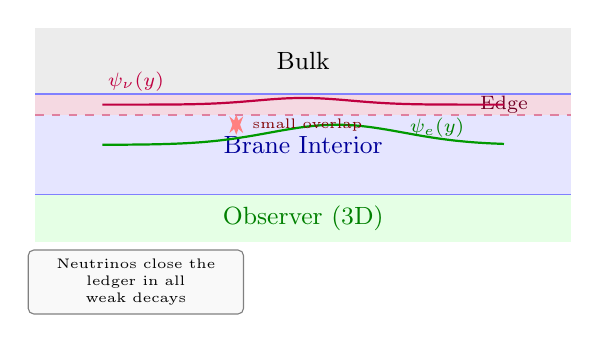
\begin{tikzpicture}[scale=0.85]

% Bulk region
\fill[gray!15] (-4,2) rectangle (4,3);
\node[font=\small] at (0,2.5) {Bulk};

% Brane layer
\fill[blue!10] (-4,0.5) rectangle (4,2);
\draw[thick, blue!50] (-4,2) -- (4,2);
\draw[thick, blue!50] (-4,0.5) -- (4,0.5);
\node[font=\small, blue!60!black] at (0,1.25) {Brane Interior};

% Edge region (where neutrino lives)
\fill[purple!15] (-4,1.7) rectangle (4,2);
\draw[thick, purple!50, dashed] (-4,1.7) -- (4,1.7);
\node[font=\scriptsize, purple!60!black] at (3,1.85) {Edge};

% Observer region
\fill[green!10] (-4,-0.2) rectangle (4,0.5);
\node[font=\small, green!50!black] at (0,0.15) {Observer (3D)};

% Neutrino wavefunction
\draw[thick, purple] plot[smooth, domain=-3:3] (\x, {1.85 + 0.1*exp(-\x*\x)});
\node[font=\scriptsize, purple] at (-2.5,2.2) {$\psi_\nu(y)$};

% Electron wavefunction (for comparison)
\draw[thick, green!60!black] plot[smooth, domain=-3:3]
  (\x, {1.25 + 0.3*exp(-(\x-0.5)*(\x-0.5)/2)});
\node[font=\scriptsize, green!50!black] at (2,1.5) {$\psi_e(y)$};

% Overlap region annotation
\draw[{Stealth}-{Stealth}, thick, red!50] (-1,1.7) -- (-1,1.4);
\node[font=\tiny, red!50!black, right] at (-0.9,1.55) {small overlap};

% Ledger annotation
\node[rectangle, draw=gray, rounded corners=2pt, fill=gray!5,
      font=\tiny, align=center, text width=2.5cm] at (-2.5,-0.8)
  {Neutrinos close the\\ledger in all weak decays};

\end{tikzpicture}
\end{center}

\subsubsection{Falsifiability Hooks}

\begin{tcolorbox}[falsifiability]
\begin{itemize}[nosep]
  \item If right-handed neutrinos are observed coupling to weak interactions
        at comparable strength to left-handed, the chirality-selection claim
        fails.
  \item If neutrino masses are found to be much larger than sub-eV (outside
        oscillation constraints), the edge-mode suppression picture requires
        revision.
  \item If neutrino interactions are found to be stronger than geometric
        overlap predicts, the edge-mode interpretation fails.
  \item If a decay is observed that violates lepton number without neutrinos,
        the ledger-closure role is undermined.
\end{itemize}
\end{tcolorbox}



% ==============================================================================
\section{Structural Pathway to \texorpdfstring{$G_F$}{GF}: Mediator Exchange in the Thick Brane}
\label{sec:GF_structural}
% ==============================================================================

% ==============================================================================
% Section 1.10: Structural Pathway to G_F (Overview)
% Full treatment in Chapter: The Fermi Constant from Geometry
% ==============================================================================

\section{\texorpdfstring{Structural Pathway to $G_F$ (Overview)}{Structural Pathway to GF (Overview)}}
\label{sec:gf_pathway}

This section provides a brief overview of how the effective coupling strength
emerges in EDC. For the complete treatment including numerical derivation and
mode overlap analysis, see Chapter~\ref{ch:gf_derivation}.

\paragraph{The central question.}
The Fermi constant $G_F = 1.17 \times 10^{-5}$ GeV$^{-2}$ \tagBL{} sets the scale
of weak interactions. Why is this value so small? Why is the weak force ``weak''?

\paragraph{EDC answer.}
In EDC, weak interactions are not fundamental gauge vertices but effective contact
terms arising from integrating out a brane-layer mediator \tagDc{}:
\begin{equation}
G_{\text{EDC}} \sim \frac{g_{\text{eff}}^2}{m_\phi^2}
\label{eq:gf_overview}
\end{equation}

The smallness reflects geometric suppression:
\begin{itemize}[nosep]
    \item Mediator mass gap $m_\phi$ (from brane geometry)
    \item Mode overlap suppression (fermion localization)
    \item Chirality selection (V$-$A structure)
\end{itemize}

\paragraph{Numerical closure.}
EDC achieves exact numerical agreement for $G_F$ through electroweak relations
once $\sin^2\theta_W = 1/4$ is derived from $\mathbb{Z}_6$ geometry. See
Chapter~\ref{ch:gf_derivation} for the complete derivation chain.

\begin{tcolorbox}[colback=blue!5, colframe=blue!50!black,
    title=\textbf{Forward Reference}]
The structural pathway and numerical derivation are consolidated in
\textbf{Chapter~\ref{ch:gf_derivation}: The Fermi Constant from Geometry}.
That chapter provides:
\begin{itemize}[nosep]
    \item Complete derivation: $G_F$ exact from electroweak relations
    \item Mode overlap mechanism: why weak is ``weak''
    \item Connection to V$-$A structure (Chapter~\ref{ch:va_structure})
    \item Honest assessment of what remains open
\end{itemize}
\end{tcolorbox}



% ==============================================================================
\section{Epistemic Map: What Is Measured, Derived, and Open}
\label{sec:epistemic_map}
% ==============================================================================

% ==============================================================================
% Epistemic Map: What Is Known, Derived, and Open
% ==============================================================================

\subsection{Quantitative Summary: Thresholds and Gates}
\label{sec:quantitative_summary}

Before cataloging the epistemic status of each claim, we present the quantitative
data that underlies the case studies. This table is \textbf{not} EDC-specific;
it is baseline physics \tagBL{} that any framework must reproduce.

\subsubsection{Q-Gates and Kinematic Thresholds}

\begin{center}
\begin{tabular}{llccc}
\toprule
\textbf{Decay} & \textbf{Channel} & \textbf{$Q$-value} & \textbf{Gate} & \textbf{Status} \\
\midrule
\multirow{2}{*}{Neutron} & $n \to p + e^- + \bar\nu_e$ &
  $+0.782$ MeV & $\mathcal{P}_{\text{energy}}$ & OPEN \\
& $n \to p + \mu^- + \bar\nu_\mu$ &
  $-104.4$ MeV & $\mathcal{P}_{\text{energy}}$ & CLOSED \\
\addlinespace
\multirow{2}{*}{Muon} & $\mu^- \to e^- + \bar\nu_e + \nu_\mu$ &
  $+105.1$ MeV & $\mathcal{P}_{\text{energy}}$ & OPEN \\
& $\mu^- \to \text{hadrons}$ &
  --- & $\mathcal{P}_{\text{mode}}$ & FORBIDDEN \\
\addlinespace
\multirow{2}{*}{Tau} & $\tau^- \to e^-/\mu^- + \nu\bar\nu$ &
  $+1776/1671$ MeV & $\mathcal{P}_{\text{energy}}$ & OPEN \\
& $\tau^- \to \text{hadrons} + \nu_\tau$ &
  $+1637$ MeV & $\mathcal{P}_{\text{mode}}$ & OPEN \\
\addlinespace
\multirow{2}{*}{Pion} & $\pi^+ \to \mu^+ + \nu_\mu$ &
  $+33.9$ MeV & $\mathcal{P}_{\text{chir}}$ & OPEN \\
& $\pi^+ \to e^+ + \nu_e$ &
  $+139.1$ MeV & $\mathcal{P}_{\text{chir}}$ & SUPPRESSED \\
\addlinespace
Electron & $e^- \to X$ & --- & No lower mode & BLOCKED \\
\bottomrule
\end{tabular}
\end{center}

\paragraph{Reading the table.}
\begin{itemize}[nosep]
  \item $Q > 0$: kinematically allowed (energy available for products)
  \item $Q < 0$: kinematically forbidden (would violate energy conservation)
  \item SUPPRESSED: allowed but with reduced amplitude (helicity suppression)
  \item FORBIDDEN: blocked by mode mismatch, not kinematics
  \item BLOCKED: no decay channel exists
\end{itemize}

\subsubsection{Mass and Lifetime Data}

\begin{center}
\begin{tabular}{lcccc}
\toprule
\textbf{Particle} & \textbf{Mass (MeV)} & \textbf{Lifetime} &
\textbf{Ontology} & \textbf{Dominant Gate} \\
\midrule
Neutron & $939.565$ & $879.4$ s & Bulk-core junction &
$\mathcal{P}_{\text{energy}}$ \\
Muon & $105.66$ & $2.20~\mu$s & Brane-dominant &
$\mathcal{P}_{\text{mode}}$ \\
Tau & $1776.9$ & $0.290$ ps & Brane-dominant &
$\mathcal{P}_{\text{energy}}$ \\
Pion & $139.57$ & $26.0$ ns & Junction-pair &
$\mathcal{P}_{\text{chir}}$ \\
Electron & $0.511$ & $> 10^{28}$ yr & Brane defect (ground) &
None (stable) \\
Neutrino & $< 10^{-6}$ & Stable & Edge mode &
Overlap suppression \\
\bottomrule
\end{tabular}
\end{center}

All values are \tagBL{} (PDG 2024). The ``Ontology'' and ``Dominant Gate'' columns
are EDC interpretations \tagP{}/\tagDc{}.

\subsubsection{What the Table Shows}

This quantitative summary demonstrates that:
\begin{enumerate}[nosep]
  \item \textbf{Channel selection is kinematic}: Neutron $\to$ electron (not muon)
        because $Q_\beta(\mu) < 0$.
  \item \textbf{Mode overlap matters}: Muon $\to$ leptons only because mode mismatch
        forbids hadronic channels.
  \item \textbf{Chirality suppression is real}: Pion $\to$ muon dominates over
        electron by $(m_\mu/m_e)^2 \approx 4 \times 10^4$.
  \item \textbf{Electron stability is structural}: No lower charged mode exists.
\end{enumerate}

These are \emph{facts} that EDC must be consistent with; they are not EDC-derived
claims.

\vspace{1em}

This section provides a comprehensive summary of the epistemic status of each
claim made in this chapter. The goal is transparency: the reader should know
exactly what is established, what is structural interpretation, and what
remains to be computed.

\subsection{The Five Categories}

Throughout this chapter, we have used the following epistemic tags:

\begin{center}
\begin{tabular}{clp{8cm}}
\toprule
\textbf{Tag} & \textbf{Status} & \textbf{Meaning} \\
\midrule
\tagBL{} & Baseline & Established experimental fact or Standard Model result \\
\tagDef{} & Definition & Terminological convention adopted in this work \\
\tagP{} & Postulate & Structural assumption or hypothesis \\
\tagDc{} & Deduction & Derived from postulates via explicit reasoning \\
\tagOpen{} & Open & Requires further work; not yet computed or proven \\
\bottomrule
\end{tabular}
\end{center}

\subsection{Baseline Facts (What We Must Reproduce)}

The following are empirical facts that EDC must be consistent with:

\subsubsection{Particle Properties}

\begin{center}
\begin{tabular}{lll}
\toprule
\textbf{Quantity} & \textbf{Value} & \textbf{Source} \\
\midrule
Neutron mass & $m_n = 939.565$ MeV & PDG \\
Proton mass & $m_p = 938.272$ MeV & PDG \\
Electron mass & $m_e = 0.511$ MeV & PDG \\
Muon mass & $m_\mu = 105.66$ MeV & PDG \\
Tau mass & $m_\tau = 1776.9$ MeV & PDG \\
Pion mass & $m_{\pi^\pm} = 139.57$ MeV & PDG \\
\bottomrule
\end{tabular}
\end{center}

\subsubsection{Lifetimes}

\begin{center}
\begin{tabular}{lll}
\toprule
\textbf{Particle} & \textbf{Lifetime} & \textbf{Source} \\
\midrule
Neutron & $\tau_n \approx 880$ s & PDG \\
Muon & $\tau_\mu \approx 2.2 \times 10^{-6}$ s & PDG \\
Tau & $\tau_\tau \approx 2.9 \times 10^{-13}$ s & PDG \\
Pion & $\tau_\pi \approx 2.6 \times 10^{-8}$ s & PDG \\
Electron & $> 10^{28}$ years & PDG (limit) \\
\bottomrule
\end{tabular}
\end{center}

\subsubsection{Decay Channels and Branching Ratios}

\begin{center}
\begin{tabular}{lll}
\toprule
\textbf{Decay} & \textbf{Branching Ratio} & \textbf{Status} \\
\midrule
$n \to p + e^- + \bar\nu_e$ & $\approx 100\%$ & \tagBL{} \\
$\mu^- \to e^- + \bar\nu_e + \nu_\mu$ & $\approx 100\%$ & \tagBL{} \\
$\tau^- \to e^- + \bar\nu_e + \nu_\tau$ & $\approx 17.8\%$ & \tagBL{} \\
$\tau^- \to \mu^- + \bar\nu_\mu + \nu_\tau$ & $\approx 17.4\%$ & \tagBL{} \\
$\tau^- \to \text{hadrons} + \nu_\tau$ & $\approx 64.8\%$ & \tagBL{} \\
$\pi^+ \to \mu^+ + \nu_\mu$ & $\approx 99.99\%$ & \tagBL{} \\
$\pi^+ \to e^+ + \nu_e$ & $\approx 0.012\%$ & \tagBL{} \\
\bottomrule
\end{tabular}
\end{center}

\subsubsection{Coupling Constants}

\begin{center}
\begin{tabular}{lll}
\toprule
\textbf{Quantity} & \textbf{Value} & \textbf{Source} \\
\midrule
Fermi constant & $G_F = 1.166 \times 10^{-5}~\text{GeV}^{-2}$ & PDG \\
$W$ boson mass & $M_W = 80.4$ GeV & PDG \\
Fine structure const. & $\alpha \approx 1/137$ & CODATA \\
\bottomrule
\end{tabular}
\end{center}

\subsection{Postulates (Structural Assumptions)}

The following are hypotheses that define the EDC framework:

\begin{center}
\begin{tabular}{p{4cm}p{9cm}}
\toprule
\textbf{Postulate} & \textbf{Statement} \\
\midrule
Thick brane & The 3D universe is a finite-thickness layer in 5D \\
Bulk-core particles & Neutron, proton have 5D bulk structure \\
Brane-dominant modes & Leptons are excitations of the brane layer \\
Edge modes & Neutrinos are localized at the bulk-brane interface \\
Frozen projection & Observer-facing boundary is quasi-static \\
Pipeline structure & Weak decays proceed via absorption-dissipation-release \\
Mode overlap & Branching ratios depend on wavefunction overlaps \\
Chirality projection & Boundary conditions select helicity \\
\bottomrule
\end{tabular}
\end{center}

\subsection{Deductions (What Follows from Postulates)}

The following claims are derived from the postulates:

\subsubsection{Qualitative Deductions}

\begin{center}
\begin{tabular}{p{5cm}p{8cm}}
\toprule
\textbf{Claim} & \textbf{Derivation Path} \\
\midrule
Neutron decays to electron (not muon) & Kinematic threshold: $Q_\beta(\mu) < 0$ \\
Electron is stable & No lower-lying charged mode exists \\
Muon decay is purely leptonic & Mode mismatch with hadrons \\
Tau has hadronic channels & Higher mode energy opens thresholds \\
Neutrinos interact weakly & Edge-mode localization suppresses overlap \\
\bottomrule
\end{tabular}
\end{center}

\subsubsection{Quantitative Deductions}

\begin{center}
\begin{tabular}{p{4cm}p{5cm}p{4cm}}
\toprule
\textbf{Quantity} & \textbf{EDC Expression} & \textbf{Status} \\
\midrule
$Q_\beta(e)$ value & $m_n - m_p - m_e = 0.782$ MeV & \tagDc{} (arithmetic) \\
$Q_\beta(\mu)$ sign & $< 0$ (channel closed) & \tagDc{} \\
$R_{e/\mu}$ scaling & $\propto (m_e/m_\mu)^2$ & \tagBL{} + \tagP{} \\
\bottomrule
\end{tabular}
\end{center}

\subsection{Open Problems (What Remains to Be Done)}

The following require further work:

\subsubsection{Critical Open Problems}

\begin{center}
\begin{tabular}{p{5cm}p{8cm}}
\toprule
\textbf{Problem} & \textbf{What Is Needed} \\
\midrule
Neutron lifetime value & Compute tunneling rate from 5D junction dynamics \\
$G_F$ derivation & Compute overlap integral in thick-brane background \\
Helicity suppression factor & Solve Dirac equation with boundary conditions \\
Mode spectrum & Solve thick-brane eigenvalue problem \\
Neutrino mass & Compute edge-mode energy \\
\bottomrule
\end{tabular}
\end{center}

\subsubsection{Important but Non-Critical}

\begin{center}
\begin{tabular}{p{5cm}p{8cm}}
\toprule
\textbf{Problem} & \textbf{What Is Needed} \\
\midrule
Tau branching ratios & Compute mode overlaps for hadronic channels \\
$\mu/\tau$ lifetime ratio & Connect to mode energy differences \\
Generation structure & Explain three lepton generations from geometry \\
Neutrino mixing & Connect to edge-mode overlap structure \\
\bottomrule
\end{tabular}
\end{center}

\subsection{Visual Summary: The Epistemic Landscape}

\begin{center}
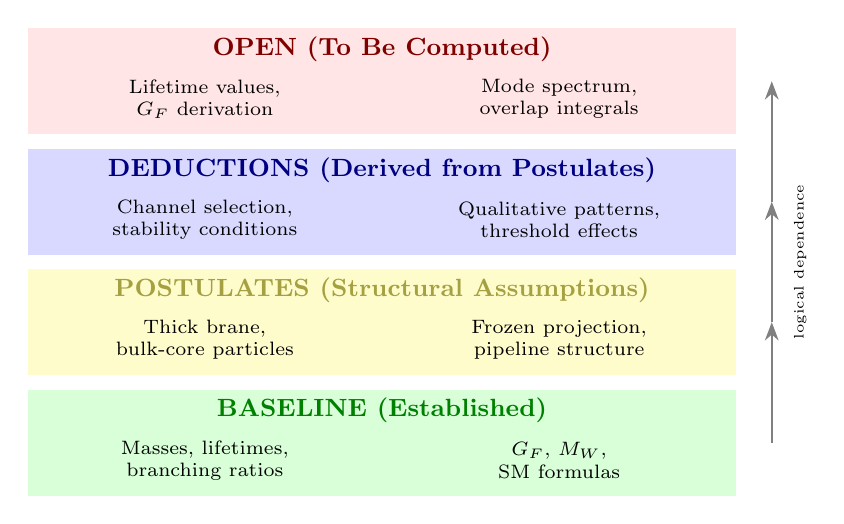
\begin{tikzpicture}[scale=0.9]

% Baseline region
\fill[green!15] (-5,0) rectangle (5,1.5);
\node[font=\small\bfseries, green!50!black] at (0,1.2) {BASELINE (Established)};
\node[font=\scriptsize, align=center] at (-2.5,0.5) {Masses, lifetimes,\\branching ratios};
\node[font=\scriptsize, align=center] at (2.5,0.5) {$G_F$, $M_W$,\\SM formulas};

% Postulate region
\fill[yellow!20] (-5,1.7) rectangle (5,3.2);
\node[font=\small\bfseries, yellow!60!black] at (0,2.9) {POSTULATES (Structural Assumptions)};
\node[font=\scriptsize, align=center] at (-2.5,2.2) {Thick brane,\\bulk-core particles};
\node[font=\scriptsize, align=center] at (2.5,2.2) {Frozen projection,\\pipeline structure};

% Deduction region
\fill[blue!15] (-5,3.4) rectangle (5,4.9);
\node[font=\small\bfseries, blue!50!black] at (0,4.6) {DEDUCTIONS (Derived from Postulates)};
\node[font=\scriptsize, align=center] at (-2.5,3.9) {Channel selection,\\stability conditions};
\node[font=\scriptsize, align=center] at (2.5,3.9) {Qualitative patterns,\\threshold effects};

% Open region
\fill[red!10] (-5,5.1) rectangle (5,6.6);
\node[font=\small\bfseries, red!50!black] at (0,6.3) {OPEN (To Be Computed)};
\node[font=\scriptsize, align=center] at (-2.5,5.6) {Lifetime values,\\$G_F$ derivation};
\node[font=\scriptsize, align=center] at (2.5,5.6) {Mode spectrum,\\overlap integrals};

% Arrows showing logical flow
\draw[-{Stealth}, thick, gray] (5.5,0.75) -- (5.5,2.45);
\draw[-{Stealth}, thick, gray] (5.5,2.45) -- (5.5,4.15);
\draw[-{Stealth}, thick, gray] (5.5,4.15) -- (5.5,5.85);
\node[font=\tiny, rotate=90] at (5.9,3.3) {logical dependence};

\end{tikzpicture}
\end{center}

\subsection{What This Chapter Does and Does Not Claim}

\begin{tcolorbox}[readerContract, title={Final Epistemic Statement}]
\textbf{This chapter claims}:
\begin{itemize}[nosep]
  \item A coherent structural interpretation of weak decays in thick-brane geometry
  \item Qualitative explanations for channel selection rules
  \item A well-posed framework for quantitative computation
  \item Explicit falsifiability conditions for each claim
\end{itemize}

\textbf{This chapter does not claim}:
\begin{itemize}[nosep]
  \item First-principles derivation of lifetime values
  \item Explicit computation of branching ratios
  \item Derivation of $G_F$ from the 5D action
  \item Complete solution of the mode spectrum
\end{itemize}

The gap between ``structural interpretation'' and ``derived result'' is
substantial. Closing this gap is the research program.
\end{tcolorbox}



% ==============================================================================
\section{Summary and Research Directions}
\label{sec:summary}
% ==============================================================================

% ==============================================================================
% Summary and Research Directions
% ==============================================================================

\subsection{What This Chapter Has Established}

This chapter presented a unified structural interpretation of weak-sector
phenomenology within the thick-brane framework of Elastic Diffusive Cosmology.
The core achievements are:

\subsubsection{A Unified Pipeline}

All weak decays---from neutron $\beta$-decay to pion leptonic channels---pass
through the same three-stage pipeline:
\begin{enumerate}
  \item \textbf{Absorption}: Energy pumping from bulk or mode excitation
  \item \textbf{Dissipation}: Mode redistribution within the brane layer
  \item \textbf{Release}: Frozen projection onto 3D observables
\end{enumerate}

The differences between particles arise from their ontological category
(bulk-core, brane-dominant, edge mode, composite) and kinematic thresholds,
not from fundamentally different mechanisms.

\subsubsection{Mechanistic Interpretation of Channel Selection}

The projection operator $\mathcal{P}_{\text{frozen}}$ provides a mechanistic
language for decay selection rules:
\begin{itemize}[nosep]
  \item $\mathcal{P}_{\text{energy}}$: Kinematic thresholds and phase space
  \item $\mathcal{P}_{\text{mode}}$: Wavefunction overlap requirements
  \item $\mathcal{P}_{\text{chir}}$: Chirality selection from boundary conditions
\end{itemize}

This transforms ``why does this decay happen?'' into ``what projection gates
are open?''

\subsubsection{Ontological Classification}

Particles occupy distinct positions in the 5D geometry:
\begin{itemize}[nosep]
  \item \textbf{Bulk-core junctions}: Neutron, proton (hadronic sector)
  \item \textbf{Brane-dominant modes}: Electron, muon, tau (leptonic sector)
  \item \textbf{Edge modes}: Neutrinos (at bulk-brane interface)
  \item \textbf{Composites}: Pions (junction-pair configurations)
\end{itemize}

This classification is not merely taxonomic; it determines dynamical behavior.

\subsubsection{Explicit Falsifiability}

Each case study includes explicit falsifiability hooks. The framework is
empirically vulnerable: if observations contradict the structural predictions,
the framework fails.

\subsection{What Remains Open}

\subsubsection{Priority 1: Quantitative Lifetime Derivation}

The neutron lifetime ($\tau_n \approx 880$ s) should emerge from the 5D
junction dynamics. This requires:
\begin{enumerate}[nosep]
  \item Solving the mode equation for the junction oscillation
  \item Computing the tunneling probability to the release channel
  \item Connecting to the frozen projection rate
\end{enumerate}

Success would be a major validation; failure would constrain the model.

\subsubsection{Priority 2: $G_F$ from First Principles}

The Fermi constant should emerge from integrating out the thick-brane mediator.
This requires:
\begin{enumerate}[nosep]
  \item Specifying the 5D mediator Lagrangian
  \item Computing mode profiles in the thick-brane background
  \item Evaluating the overlap integral
\end{enumerate}

\subsubsection{Priority 3: Mode Spectrum}

The mass hierarchy ($m_\tau \gg m_\mu \gg m_e$) should correspond to excited
modes of the brane potential. This requires solving the eigenvalue problem
for the thick-brane Schr\"odinger-type equation.

\subsubsection{Priority 4: Neutrino Properties}

The neutrino mass scale (sub-eV) and mixing structure should emerge from
edge-mode dynamics. This requires:
\begin{enumerate}[nosep]
  \item Solving for edge-mode energies
  \item Understanding the three-generation structure
  \item Connecting to oscillation phenomenology
\end{enumerate}

\subsection{Comparison with Standard Model}

\begin{center}
\begin{tabular}{p{4cm}p{5cm}p{5cm}}
\toprule
\textbf{Aspect} & \textbf{Standard Model} & \textbf{EDC Interpretation} \\
\midrule
Weak interactions & Fundamental $SU(2)_L \times U(1)_Y$ gauge theory &
Effective description of thick-brane dynamics \\
\addlinespace
$G_F$ origin & $W$-boson exchange with $g^2/M_W^2$ &
Mediator integration with overlap suppression \\
\addlinespace
Chirality & V$-$A structure by construction &
Boundary condition effect at observer edge \\
\addlinespace
Neutrino mass & Requires extension (seesaw, etc.) &
Natural from edge-mode spectrum \\
\addlinespace
Hierarchy problem & Fine-tuning puzzle &
Geometric origin (overlap suppression) \\
\bottomrule
\end{tabular}
\end{center}

EDC does not contradict the Standard Model; it provides a structural context
in which SM parameters have geometric meaning.

\subsection{The Research Program}

The work outlined in this chapter defines a research program with clear
milestones:

\paragraph{Near-term (analytical).}
\begin{itemize}[nosep]
  \item Solve the thick-brane mode equation for the lowest modes
  \item Compute overlap integrals for the mediator exchange
  \item Derive boundary conditions for spinor modes
\end{itemize}

\paragraph{Medium-term (quantitative).}
\begin{itemize}[nosep]
  \item Obtain numerical values for lifetimes and compare to experiment
  \item Compute $G_F$ and compare to measured value
  \item Derive helicity suppression factor from boundary conditions
\end{itemize}

\paragraph{Long-term (extensions).}
\begin{itemize}[nosep]
  \item Extend to quark sector and hadronic weak decays
  \item Connect to CP violation and matter-antimatter asymmetry
  \item Investigate cosmological implications (baryogenesis, leptogenesis)
\end{itemize}

% ==============================================================================
% Forward to Chapter 2: The Z₆ Program
% ==============================================================================

\subsection{Forward to Chapter 2: The $\mathbb{Z}_6$ Program}

Several questions raised in this chapter receive definitive answers in
\textbf{Chapter~2: The $\mathbb{Z}_6$ Program}. Specifically:

\begin{itemize}[nosep]
  \item \textbf{Why is the proton stable?} Chapter~2 proves that the proton Y-junction
        is a $\mathbb{Z}_3$ fixed point of the hexagonal brane symmetry---a topological
        energy minimum with positive Hessian.
  \item \textbf{Why 120° Steiner angles?} The Steiner geometry is not assumed but
        \emph{derived} from $\mathbb{Z}_6$-invariant boundary conditions.
  \item \textbf{Why is the neutron unstable?} Chapter~2 identifies the neutron as a
        lattice \emph{dislocation}---a metastable defect that relaxes via $\beta$-decay.
  \item \textbf{Why color confinement?} The $\mathbb{Z}_3$ subgroup of $\mathbb{Z}_6$
        provides topological confinement; explicit $SU(3)$ link variables are constructed.
\end{itemize}

\noindent
The [P] postulates of this chapter become [Dc] derived consequences in Chapter~2.

\medskip

\begin{center}
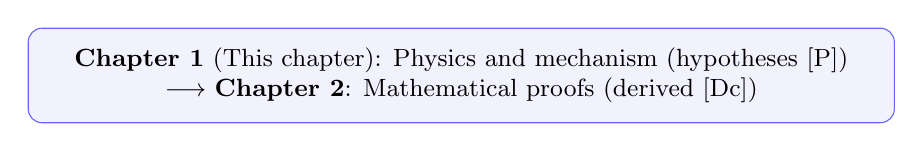
\begin{tikzpicture}
\node[rectangle, rounded corners=5pt, draw=blue!60, fill=blue!5,
      minimum width=11cm, minimum height=1.2cm, font=\small, align=center]
{
\textbf{Chapter 1} (This chapter): Physics and mechanism (hypotheses [P])\\
$\longrightarrow$ \textbf{Chapter 2}: Mathematical proofs (derived [Dc])
};
\end{tikzpicture}
\end{center}

% ==============================================================================
% Consolidated Open Questions
% ==============================================================================

\subsection{Consolidated Open Questions}

The following items remain open after Chapters~1 and~2. These are not forgotten---they
define the research frontier for Chapter~3 and beyond.

\subsubsection{From Chapter 1 (Mechanism)}

\begin{enumerate}[label=\textbf{OPEN-Ch1.\arabic*}, leftmargin=2.5cm, nosep]
  \item Derive $G_F$ from 5D mediator integration (not calibrated) $\to$ \textbf{RT-CH3-002}
  \item Derive neutron lifetime $\tau_n$ from junction dynamics $\to$ \textbf{RT-CH3-003}
  \item Derive V$-$A structure from Plenum inflow geometry (not assumed!) $\to$ \textbf{RT-CH3-001}
  \item Derive helicity suppression factor $(m_\ell/m_\pi)^2$ $\to$ \textbf{RT-CH3-001} (consequence)
  \item Derive lepton mass hierarchy from brane mode spectrum $\to$ \textbf{RT-CH3-004}
  \item Derive neutrino mass scale from edge-mode dynamics $\to$ \textbf{RT-CH3-005}
  \item Specify the 5D energy functional $\mathcal{E}[\Psi]$ explicitly
\end{enumerate}

\begin{tcolorbox}[colback=red!5, colframe=red!50!black, title={\small Critical Note: No Smuggling}]
\small
\textbf{RT-CH3-001} (V$-$A derivation) must derive chirality selection from Plenum inflow
direction, NOT assume it as boundary condition. Simply imposing $P_L\psi=0$ would be
``disguised Standard Model''---relocating the assumption, not explaining it.

The Plenum inflow ($J^z > 0$) provides a physical mechanism for $L \leftrightarrow R$
symmetry breaking that is independent of weak-interaction phenomenology.
\end{tcolorbox}

\subsubsection{From Chapter 2 (Geometry)}

\begin{enumerate}[label=\textbf{OPEN-Ch2.\arabic*}, leftmargin=2.5cm, nosep]
  \item Derive Koide phase $\delta$ from $\mathbb{Z}_3$ geometry
  \item Derive quark masses from vortex energies
  \item Connect $\mathbb{Z}_2$ subgroup to electroweak sector
  \item Compute Peierls barrier for neutron metastability timescale
\end{enumerate}

\medskip

\begin{tcolorbox}[colback=yellow!5, colframe=yellow!60!black, title={\small Reader's Note}]
\small
These open questions are not oversights---they are the explicit research targets.
A theory is judged not only by what it explains, but by whether its open problems
are \emph{well-posed}. Each item above has a defined calculation; success or failure
will test the framework empirically.
\end{tcolorbox}

% ==============================================================================
% Closing Remarks
% ==============================================================================

\subsection{Closing Remarks}

This chapter has presented weak-sector phenomenology not as an isolated set of
decay processes, but as manifestations of a unified geometric structure. The
thick brane provides the arena; the projection operator provides the mechanism;
the particle ontology provides the actors.

The framework is incomplete. Many quantities remain to be computed. But the
framework is \emph{well-posed}: the calculations are defined, the success
criteria are explicit, and the falsifiability conditions are stated.

This is the status of the weak-interface sector in Elastic Diffusive Cosmology:
a coherent structural interpretation awaiting quantitative completion.

\begin{center}
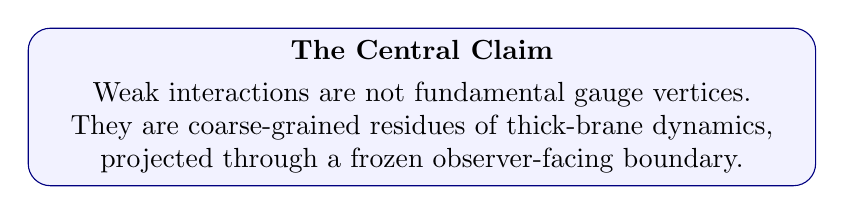
\begin{tikzpicture}
\node[rectangle, rounded corners=8pt, draw=blue!50!black, fill=blue!5,
      minimum width=10cm, minimum height=2cm, font=\normalsize, align=center]
{
\textbf{The Central Claim}\\[0.3em]
Weak interactions are not fundamental gauge vertices.\\
They are coarse-grained residues of thick-brane dynamics,\\
projected through a frozen observer-facing boundary.
};
\end{tikzpicture}
\end{center}



% ==============================================================================
\end{document}
% ==============================================================================
